%% ----------------------------------------------------------------
%% Thesis.tex -- MAIN FILE (the one that you compile with LaTeX)
%% ---------------------------------------------------------------- 

% Set up the document
\documentclass[a4paper, 11pt, oneside]{Thesis}  % Use the "Thesis" style, based on the ECS Thesis style by Steve Gunn
\graphicspath{{Figures/}}  % Location of the graphics files (set up for graphics to be in PDF format)

% Include any extra LaTeX packages required
\usepackage[square, numbers, comma, sort&compress]{natbib}  % Use the "Natbib" style for the references in the Bibliography
\usepackage{verbatim}  % Needed for the "comment" environment to make LaTeX comments
\usepackage{vector}  % Allows "\bvec{}" and "\buvec{}" for "blackboard" style bold vectors in maths
\hypersetup{urlcolor=blue, colorlinks=true}  % Colours hyperlinks in blue, but this can be distracting if there are many links.

%% ----------------------------------------------------------------
\begin{document}
\frontmatter	  % Begin Roman style (i, ii, iii, iv...) page numbering

% Set up the Title Page
\title  {Thesis Title}
\authors  {\texorpdfstring
            {\href{your web site or email address}{Author Name}}
            {Author Name}
            }
\addresses  {\groupname\\\deptname\\\univname}  % Do not change this here, instead these must be set in the "Thesis.cls" file, please look through it instead
\date       {\today}
\subject    {}
\keywords   {}

\maketitle
%% ----------------------------------------------------------------

\setstretch{1.3}  % It is better to have smaller font and larger line spacing than the other way round

% Define the page headers using the FancyHdr package and set up for one-sided printing
\fancyhead{}  % Clears all page headers and footers
\rhead{\thepage}  % Sets the right side header to show the page number
\lhead{}  % Clears the left side page header

\pagestyle{fancy}  % Finally, use the "fancy" page style to implement the FancyHdr headers

%% ----------------------------------------------------------------
% Declaration Page required for the Thesis, your institution may give you a different text to place here
\Declaration{

\addtocontents{toc}{\vspace{1em}}  % Add a gap in the Contents, for aesthetics

I, AUTHOR NAME, declare that this thesis titled, `THESIS TITLE' and the work presented in it are my own. I confirm that:

\begin{itemize} 
\item[\tiny{$\blacksquare$}] This work was done wholly or mainly while in candidature for a research degree at this University.
 
\item[\tiny{$\blacksquare$}] Where any part of this thesis has previously been submitted for a degree or any other qualification at this University or any other institution, this has been clearly stated.
 
\item[\tiny{$\blacksquare$}] Where I have consulted the published work of others, this is always clearly attributed.
 
\item[\tiny{$\blacksquare$}] Where I have quoted from the work of others, the source is always given. With the exception of such quotations, this thesis is entirely my own work.
 
\item[\tiny{$\blacksquare$}] I have acknowledged all main sources of help.
 
\item[\tiny{$\blacksquare$}] Where the thesis is based on work done by myself jointly with others, I have made clear exactly what was done by others and what I have contributed myself.
\\
\end{itemize}
 
 
Signed:\\
\rule[1em]{25em}{0.5pt}  % This prints a line for the signature
 
Date:\\
\rule[1em]{25em}{0.5pt}  % This prints a line to write the date
}
\clearpage  % Declaration ended, now start a new page

%% ----------------------------------------------------------------
% The "Funny Quote Page"
\pagestyle{empty}  % No headers or footers for the following pages

\null\vfill
% Now comes the "Funny Quote", written in italics
\textit{``Write a funny quote here.''}

\begin{flushright}
If the quote is taken from someone, their name goes here
\end{flushright}

\vfill\vfill\vfill\vfill\vfill\vfill\null
\clearpage  % Funny Quote page ended, start a new page
%% ----------------------------------------------------------------

% The Abstract Page
\addtotoc{Abstract}  % Add the "Abstract" page entry to the Contents
\abstract{
\addtocontents{toc}{\vspace{1em}}  % Add a gap in the Contents, for aesthetics

The Thesis Abstract is written here (and usually kept to just this page). The page is kept centered vertically so can expand into the blank space above the title too\ldots

}

\clearpage  % Abstract ended, start a new page
%% ----------------------------------------------------------------

\setstretch{1.3}  % Reset the line-spacing to 1.3 for body text (if it has changed)

% The Acknowledgements page, for thanking everyone
\acknowledgements{
\addtocontents{toc}{\vspace{1em}}  % Add a gap in the Contents, for aesthetics

The acknowledgements and the people to thank go here, don't forget to include your project advisor\ldots

}
\clearpage  % End of the Acknowledgements
%% ----------------------------------------------------------------

\pagestyle{fancy}  %The page style headers have been "empty" all this time, now use the "fancy" headers as defined before to bring them back


%% ----------------------------------------------------------------
\lhead{\emph{Contents}}  % Set the left side page header to "Contents"
\tableofcontents  % Write out the Table of Contents

%% ----------------------------------------------------------------
\lhead{\emph{List of Figures}}  % Set the left side page header to "List if Figures"
\listoffigures  % Write out the List of Figures

%% ----------------------------------------------------------------
\lhead{\emph{List of Tables}}  % Set the left side page header to "List of Tables"
\listoftables  % Write out the List of Tables

%% ----------------------------------------------------------------
\setstretch{1.5}  % Set the line spacing to 1.5, this makes the following tables easier to read
\clearpage  % Start a new page
\lhead{\emph{Abbreviations}}  % Set the left side page header to "Abbreviations"
\listofsymbols{ll}  % Include a list of Abbreviations (a table of two columns)
{
% \textbf{Acronym} & \textbf{W}hat (it) \textbf{S}tands \textbf{F}or \\
\textbf{LAH} & \textbf{L}ist \textbf{A}bbreviations \textbf{H}ere \\

}

%% ----------------------------------------------------------------
\clearpage  % Start a new page
\lhead{\emph{Physical Constants}}  % Set the left side page header to "Physical Constants"
\listofconstants{lrcl}  % Include a list of Physical Constants (a four column table)
{
% Constant Name & Symbol & = & Constant Value (with units) \\
Speed of Light & $c$ & $=$ & $2.997\ 924\ 58\times10^{8}\ \mbox{ms}^{-\mbox{s}}$ (exact)\\

}

%% ----------------------------------------------------------------
\clearpage  %Start a new page
\lhead{\emph{Symbols}}  % Set the left side page header to "Symbols"
\listofnomenclature{lll}  % Include a list of Symbols (a three column table)
{
% symbol & name & unit \\
$a$ & distance & m \\
$P$ & power & W (Js$^{-1}$) \\
& & \\ % Gap to separate the Roman symbols from the Greek
$\omega$ & angular frequency & rads$^{-1}$ \\
}
%% ----------------------------------------------------------------
% End of the pre-able, contents and lists of things
% Begin the Dedication page

\setstretch{1.3}  % Return the line spacing back to 1.3

\pagestyle{empty}  % Page style needs to be empty for this page
\dedicatory{For/Dedicated to/To my\ldots}

\addtocontents{toc}{\vspace{2em}}  % Add a gap in the Contents, for aesthetics


%% ----------------------------------------------------------------
\mainmatter	  % Begin normal, numeric (1,2,3...) page numbering
\pagestyle{fancy}  % Return the page headers back to the "fancy" style

% Include the chapters of the thesis, as separate files
% Just uncomment the lines as you write the chapters

\chapter{Introduction}  \label{Chapter1}
\lhead{Chapter 1. \emph{Introduction}}

Supernoavea (SN) are extremely luminous stellar explosions. At their brightest, they can outshine the galaxy that gave birth to them, making them visible at great distances and far back in time. SNe have been observed by stargazers since the the dawn of human kind. By studying nebulea formed as remnants of past explosions, as well as ancient records we know that human history is filled with observations of 'guest stars' most famously in 1054 where the SN, now observed as the Crab nebula, has been recorded in China, seen to be brighter than the full moon at night and visible during the day, as well as the SN1574, known as the Tycho SN and SN1604 in the end of the 16th and beginning of 17th centuries.

Despite their early observations, the term `Supernova' was not coined until 1934 when \citet{Baade1934} were able to estimate their absolute magnitudes. Using Cepheid variables, they measured the distance to several SN host galaxies and found them to be significantly greater then those of classical `Novae'. The prefix `super' reflects their absolute luminosity which must be much greater than that of novea to explain their bright observed magnitudes.

\section{SN classification}
At that point of their discovery, little has been known about the properties and physical origin of these extreme objects, largely due to the sparcity of their observations at that time \citep{Zwicky1938}. In the years to come, many generations of astronomers built increasingly larger and more sensitive surveys, observing thousands of SNe to date \citep{Alsabti2017}. With this came our understanding of the various types and flavours of SNe and the breath of the variation in the objects that can give rise to such brilliant explosions.

\subsection{SN\,Ia}
Perhaps the most well understood and most heavily studies class are the thermonuclear SNe. While a number of their subclasses exists \citep[amongst others: SN\,.Ia, SN\'Iax, SN\,Ia-91T, SN\,Ia-91bg][]{Alsabti2017} all of these objects likely share a similar physical origin to the main SN\,Ia class. There are competting theories explaining their origin, both describe an thermonuclear explosion of a white dwarf (WD) star, but differing in the mechanism which triggers the ignition. In the single-degenerate scenario \citep{Whelan1973} a WD, in a binary system, accreates matter from a main-sequence or red giant star until it reaches the Chandrasekhar limit defined as the point at which the electron degeneracy presure can no longer support the star against a gravitational collapse, resulting in an increase in pressure and subsequent thermonuclear ignition of its core. The alternative explanation suggests that instead of a single WD, a binary WD system interacts internally, spiralling down through the release of gravitational waves, resulting in their eventual `collision triggering a powerful sufficient to ignite the degenerate matter even at sub-Chandrasekhar limit masses \citep{Iben1984}.

Both of the above mechanisms result in a production of $\sim$0.7M$_\odot)$ of Ni56 \citep{Scalzo2014} which decays radioactively to Co56 and Fe56 producing a vast quantity of high energy Gamma radiation, which is subsequently reproduced by the SN ejecta into visible light. Cosmology

\subsection{SN\,II}
The origin of SN\,II in many ways mirrors that of SN\,Ia; both are the result of the end point of the evolution and the death of their progenitor star. SN\,II are born when a $>$8Msun star exhausts all of its nuclear fuel at the end of the iron burning phase [CITE]. At that point the core is supported purely by the electron degeneracy pressure and collapses shortly afterwards into neutron star under the gravitational pressure of the outter layers of the star. The infalling shells rebound of the, now, solid core and are further energised and accelerated by either the neutrinos released in the collapse of the degenerate core [CITE] or jets formed due to the accreation of the infalling matter onto the core [CITE].

In this process, only a small, in comparison to SN\,Ia, amount of the Ni56 is formed which alone could not explain neither the luminosity of these core-coolapse SNe (CCSN) nor their light curve morphologies which are offten associated with a sharp rise followed by either a long platue phase (SN\,IIP) or a linear decline (SN\,IIL) \citep{Alsabti2017}. These are the effect of Hydrogen recombination (ionised to neutral) in the outter layer of the ejecta, resulting in a blackbody like spectrum with prominant P-cygni profiles visible in the spectra. Additionally, some objects also show narrow emission lines (SN\,IIn), of mostly hydrogen, which are the result of the iteractions between the SN ejecta and extended material ejected by the progenitor star some time before the main event [CITE].

\subsection{SN\,Ib/c}
SN\,Ib/c have a very similar origins to SN\,II. They are also a result of a core collapse of a giant star but significantly they originate from larger and more `stripped' stars. These objects are often referred to as Stripped-Envelope SNe reflicting the fact that no hydrogen (SN\,Ib) nor hellium (SN\,Ic) are visible in their spectra as they were removed from the surface of the star by either winds or corronal mass ejections a relatively long time period to the onset of the SN event. Some theories suggest that the stipping cannot be explained solely using wind and corronal ejections and must be a result of an interaction with a companion star [CITE].

Thanks to the higher mass of the progenitor star, these objects often result in a larger production of Ni56, resulting in a higher luminosity and a morphology which in the extreme cases can closely resemble that of a SN\,Ia. Spectroscopically, this class of SNe shows a strong formation of Oxygen and Carbon and well as small quantities of other, intermediate mass elements \citep{Filippenko1997}.

\subsection{Other subclasses}
Outside of the main, or most commonly detected, subclasses of SNe lives a number of rares and more exodic transient types. Amonst these, there is a number of intermediate classes of CCSNe that originate at the boundries of the progenitor scenarios. This includes SNIIb, SNIbn and SNIbc amongst others \citep{Alsabti2017}, however, an overlap also exists between the SN\,Ia and the interacting CCSN. SN\,Ia-CSM are one of the most luminous classes of SNe as the extreme brightness of SN\,Ia is enhanced further by the interaction of the ejecta with a layer of circumstellar material (CSM) likely ejected by the companion star \citep{Dilday2012}.

As SN surveys become more sensitive and sophisticated, the numbers of known SN classes grew as well. In recent years, higher cadance SN searches have lead to the discovery of a new class of Rapidly Evolving Transients (RAT) with an extreme variation in their peak luminosity ranging from -15 < M < -22 \citep{Pursiainen2018}. Little is yet known about their physical origins, however, their observations suggest a featureless blackbody-like spectrum, often associated with initially high temperatures followed by rapid cooling. A possible interpretation of these objects is an object which undergoes a direct collapse to a black hole, producing none or little Ni56, explaining the lack of a slowly declining light curve. In this scenario, the observed morphology is a result of the interaction between the SN shock with an extended shall of dense wind \citep{Piro2015}, similarly to an effect sometimes observed in superluminous supernovae (SLSN).

\section{Superluminous Supernovae}
Superluminous supernovae (SLSNe) are a recently identified class of transients defined as events with an absolute magnitude brighter than $-$21 ($M<-21$) \citep{Gal-Yam2012}. They appear 10-100 times brighter than normal supernova events, and form at least two distinct classes: SLSNe-II, which show signatures of interaction with CSM via hydrogen and other lines \citep{Ofek2006,Smith2006,Drake2011}, and SLSNe-I (or SLSNe-Ic), which are hydrogen-poor \citep{Quimby2011}. While SLSNe-II may naturally be explained as an extension of the fainter SN\,IIn events, the power source behind SLSNe-I remains a subject of debate \citep{Gal-Yam2012}.

SLSNe-I (SLSN; hence forth) are the protagonists of this thesis. In this section, I will introduce the observations that have led to their discovery, their spectroscopic and photometric properties as well as their host galaxies. Furthermore, I will introduce their most commonly accepted formation theories and their effect on the rate of SLSN.

\subsection{Discovery}
The observational properties of SLSNe had a strong impact on the timing of their discovery. As a rare but luminous class of transients, the probability of their detection was low in the early SN surveys in the local universe due to their lower sensitivity and search volume. The first signs of the existance of a new class of extremely luminous SNe came with the discovery of SN2005ap \citep{Quimby2007}, SN2006gy \citep{Ofek2007} and SCP06F6 \citep{Barbary2009}. In each case the distance measurements for the objects have placed them at a luminosity $\sim$100 times brighter than ordinary SNe. However, the low quality of their early light curves and spectra along with a lack other example resulted in these objects being treated more as extremes of the known classes of objects instead of a separate new class.

This picture has evolved dramatically in the last decade with the onset of a number of deep, wide field surveys such as the Texas Supernova Search \citep[TSS;][]{Quimby2006}, the Palomar Transient Factory \citep[PTF;][]{Law2009, Rau2009}, the Supernova Legacy Survey \citep[SNLS;][]{Astier2005,Guy2010,Perrett2010}, the Panoramic Survey Telescope \& Rapid Response System \citep[Pan-STARRS;][]{Kaiser2010} and the Dark Energy Survey \citep[DES;][]{Flaugher2005}. With an increased sensitivity, longer observing season and a lack of host galaxy selection bias; each one of these surveys was responsible for detecting several SLSNe, jointly shaping our current understanding of this new and exciting area of SNe research.

\subsubsection{Luminous Supernoavae}
The terms `Luminous Supernoavae' and `Superluminous Supernovae' became popular in the literature upon the discovery of SN2007bi \citep{Gal-Yam2009} during the science verification phase of PTF. Its light curve, containing only the single \textit{r}-band filter, lacked the rise time information but demonstrated a very slow decline consitant with the radioactive decay of a large mass of Ni56. At that time it was believed that such event could be a result of a Pair Instability SNe (PISN; \sref{sec:Origins}) and were therefore thought to be a new class of transients.

Following shortly from this, a number of objects were discovered with similar properties. \citet{Quimby2009} presented a sample of SNe detected by PTF along with the first, comprehensive sample of their spectra. While mostly consistant of a blue, featureless blackbody continuum, some absorption lines including CII, MgII and OII \citep[see ][for more recent line identification]{Mazzali2015} were identified in all spectra in this sample, confirming the redshifts and extreme luminosity of these events.

\subsection{Properties}
Beyond confirming their redshifts, the prominant UV spectral lines can also used to measure the expansion velocity and temperature of the photospeheres of SLSNe, measured around maximum light to be of the order of $\sim$15000km/s and $\sim$10,000K respectively. This suggests that SLSNe are a class of very energetic events powered by a internal engine capable to reenergise the ejectra to produce the observed temperature, impossible to sustain in a scenario where the SN is expanding adiobatically in absence of internal heating source.

The combination of the size of the photospere and the extreme temperatures results in a objects which are extremely luminous, particularly in the blue bands where most of their luminosity is being emmited. From the point of view of their detectibility, this makes SLSNe fantastic probes of the high redshift universe as the increasing distance modulus is partially offset by the increase in observed flux as we probe the UV SED redshifted into the visible bands.

Another, clear observable difference between SLSNe and other classes of SNe is their slow evolution \citep{Gal-Yam2009, Inserra2013, Nicholl2015a}. Their risetime of $\sim$30 days in the rest-frame amd decline times as slow as 0.01 magnites per day are vastly longer timescales than those of other luminous classes of transients inluding SN\,Ia and Gamma Ray Burst (GRB) afterglows.

\subsection{Origins} \label{sec:Origins}
The most popular model in the literature to explain SLSNe involves energy input from the spin-down of a newly-formed magnetar following a CCSN \citep{Kasen2009,Woosley2010,Inserra2013}, although alternative models involving PISN \citep{Woosley2007,Yan2015} or interaction with a hydrogen-free CSM \citep{Chevalier2011,Chatzopoulos2013,Sorokina2015} have also been proposed.

\subsubsection{Magnetar model}
The spin-down of the magnetar model postulates that the birth of a SLSN is linked with the death of an extremely massive star with a intrinsicly high angular momentum and magnetic field. As such star collapses, it formes a Magnetar, defined as a neutron star with a magnetic field of B$\sim10^{14}$G and spin period, P$\sim$1ms. As the young magnetar remains shrouded by the relatively dense ejecta in the early phases of the SN, the rapidly rotating and magnetised core interacts with the inner layers of the SN, through the process of magnetic breaking, converting some of its rotational inertial into high energy radiation. The x-rays photons produced in this process are then thermolised by the ejecta and re-emmited as the observed blackbody radiation.

A further prediction of this model is the formation of a powerful shockwave, at the birth of the magnetar, which propagates through the ejectra compressing it into a thick layer [CITE] expanding at a uniform rate \citep{Inserra2013}, unhampered by any intercations and collisions between varying velocity layers as observed in other SNe. This results in a high and stable opacity values, leading to a full trapping of the high energy radiations by the ejecta.

There is a range of observational evidence supporting this model. A number of studies have demonstrated that the total radiated bolumetric luminosity of SLSNe are consistant with the predicted energy emmited by a spid-down of a magnetar [CITE]. Furthermore, the decline phase of these SNe, which was shown to be difficult to model under other assumptions, is very well explain by the slow energy deposition into the ejecta by the magnetar. However, perhapse most intrigingly, a thorough examination of the spectra of SLSNe in \citet{Mazzali2015} showed that the existance of some of the lines could only be attributed to a non-thermal ionisation of a dense ejecta by a luminous x-ray source.

\subsubsection{Pulsating Pair Instability SN}
Amongst the alternative models describing the origin of SLSNe, PISN remain a plausible alternative, especially in the cases of some of the less luminous and slowly declining objects. PISNe have been theorised for a number of decades [CITE] and are a result of the end point of the evolution of extremely massive stars with mass, M$\sim$140M$_{odot}$. At this extreme limit, the density temerature of the core are sufficiently high to achieve rate of electron-positron pair production higher than their rate of annihilation. This results in a decrease in the pressure and subsequently a further collapse of the which in turn increase its density and temparature leading to a runnaway reaction that culminates in a thermonuclear detonation of the core, not unlike that of SN\,Ia albeit producing significantly larger quantities of the radioactive Ni56 in the process.

While the develpment of the PISN models continues, it is not unlikely that the majority of SLSNe can be explained using this model as it is believed [CITE] that such events would likely result in a red SED due to large amount of Iron produced in the explosion leading to line blanketing of the UV regions of their spectra, similarly to the effect observed in other Ni56 powered SNe.

\subsubsection{Interactions with the Circumstellar Matertial}
The interactions between the SN ejecta and Circumstellar Matertial (CSM) is a well documented and understood engine powering the luminosity of a number of classes of SNe. While it is widely accepted that SLSN-II, which contain stong signs of interactions in form of prominant hydrogen emission lines observed in their spectra, are powered through this process, essentially, placing them at the bright tail-end of the distribution of ordinary SN\,II.

A similar scenario has been suggested as the powering mechanism behind SLSN-Ic [CITE]. Here, the lack of hydrogen or helium detection in their spectra is attributed to the SN event taking place in an environment where the star has either efficiently burned all of its hydrogen or expelled it a long time before the core-collapse event, resulting in the star shrouded a CSM composed of intermediate mass elements alone. Similarly to the PISNe, this model is not believed to be the likely source of the majority of the SLSNe population due to the lack of hydrogen detections in even very late light curves, predicted by the model.

\subsection{Host Galaxies}
Additional clues about the origins and conditions required to form SLSNe also provided by the environments in which they occur: predominantly vigorously star-forming and low-metallicity dwarf galaxies \citep[e.g.,][]{Lunnan2014,Leloudas2015,Angus2016}. There are now a number of clues which suggests that this effect is a direct consequence of the scenario where the spid-down of the magnetar is responsible for the formation of these objects.

The preference for low-metallicity environments is supported by the modelling of the SLSN spectra, which favours a fairly low metal abundance \citep{Mazzali2015}. It has also been suggested [CITE] that it is unlikely for a high metalicity star to retain sufficient mass, throughtout its evolutionary cycle, to result in a SN with $\sim$40M$_{\odot}$ of ejected material. Furthermore, metalicity might be the answer to the questions raised about the formation of a star which is simultaniously extremely magnetised and rapidly rotating as such extreme objects have, to date, not been observed in the local universe.

Another driving factor behind the connection to young, metal poor, heavily star-forming dwarf galaxies is the formation rate of massive stars known to be associated with these conditions as seen locally in the Small Magellanic Cloud (SMC). If the strong preference for a young environment reflects a real physical effect, any evolution in the SLSN rate with redshift should also track the cosmic star-formation and metal enrichment history of the Universe, and the underlying evolving populations of galaxies.

\subsection{Rates}
Of particular note is the rarity of SLSN-I events. It took many years for the first events to be identified as such \citep{2007ApJ...668L..99Q,2009ApJ...690.1358B}, and for the class to be recognised \citep{2011Natur.474..487Q}, in part due to their blue and relatively featureless optical spectra. Even after several years of study, only around 25 well-observed SLSNe-I exist \citep[e.g., see compilations in][]{2014ApJ...796...87I,2015MNRAS.449.1215P,2015MNRAS.452.3869N}. Initial estimates placed the rate of SLSNe-Ic at less than one for every 1000 core collapse supernovae \citep{2011Natur.474..487Q}, and more recent studies are broadly consistent with this \citep{2013MNRAS.431..912Q,2015MNRAS.448.1206M}. However, there has been no direct measurement of the SLSN-I rate for a well-controlled optical transient survey. Such a measurement can provide constraints on progenitor models, as there must, at the very least, be a sufficient number of any putative progenitor system to produce the observed SLSN rate.

\subsection{Connection to Long GRBs}
text

\section{SN Surveys}
One of the most instrumental advances that has lead to the discovery and the development of our understanding surrounding SLSNe is the dawn of the new era of automated, untargetted wide field SN surveys. While there is now a ever growing number of such projects, I endevour to avoid the discussion of individual surveys and instead summerise their general features that impact the study of SLSNe. While it is important to discuss the benefits these projects bring, I would like to focus the attantion of this section on the limitations of the past, current, and future surveys and the impact these have on the work performed in this thesis, involving SLSN classification and their search in the high redshift universe.

\subsection{Cadances}
It is perhapse unsurprising that in the field dominated by the study of SN\,Ia and their use as cosmological probes, the large majority of surveys operated in the last two decade optomise their design to maximise the quality of their relatively short light curves. The cadances, i.e the frequency of observations, are chosen at $\sim$5\,days, sufficient to give each SN\,Ia light curve between three to five points during the critial rise phase, necessary for high precision model fitting used in the cosmological studies. A number of surveys inluding SDSS, PTF, Pan-STARRS, SNLS amonst others conform to this norm.

As rare, slowly evolving and particularly brilliant objects, SLSNe do not require the same observing criteria as their less luminous cousins. In fact, a design that would maximise their detectability would focus on lower cedance and shallower fields and instead use the telescope time to search a larger observing area. Ideally, these fields should also be placed in the parts of the sky visible for a long period of time. While surveys like this were attempted in the past (e.g SUDSS; \sref{sec:SUDSS}), they were met with particularly bad observing conditions and therefore never realising their full potential. As a result, all observations of SLSNe are limited to relatively short light curves ($\sim$5\,months), often observing the SNe at a very high signal to noise despite their low numbers.

The observing conditions have huge effect on the detection and more so on the analysis of SLSNe despite being one of the hardest aspect of survey design to account for. In the past, survey designed to follow SN only would often receive a chaotic cadance where bad weather usually results in less frequent observations. In the case of DES, where there are other components of the survey sheduled from the same pool of alocated time, unfavourable observing conditions for the element of DES requirig high imae quality often result in DES SN light curves having a denser than designed cadance, albeit with the additional data points often having much lower Signal-to-Noise (S/N) ratio.

\subsection{Differential photometry}
to Forced photometry works on the principle of selecting high quality, low Point Spread Function (PSF), reference images which are then downgraded in quality to match that of the science images containing the transients. The reference images must not contain any SN light hence they usually either predate the explosion epoch of the SN use images takes several years after the explosion epoch. Once the science and reference images are matched in image quality they are warped using SWARP [CITE] so that they photometric solutions also match. After this, the reference image is subtracted from the science image. The difference here between the quick reduction photometry and force photometry is that instead of measuring the centroids of the point sources in one image and extracting its photometry the centroids are measured in the entire series of images and then an aperture matching that of the PSF of the image is used to extract the flux count.

\section{Cosmology and Distance measurements}
The fields of Cosmology and SN researh live in a fascinating symbiaotic relationship. Without our understanding of the expansion of the universe, and variability to use it to measure distances to using redshift we would not be able to study SNe at high redshifts where estimating distances using different methods becomes difficult. Similarly, SNe provide one of the most powerful tools for studing the cosmologial parameters of the our universe, famously leading to the discovery of the accelerated expansion of the universe \citep{Riess1998,Perlmutter1997} for which Adam Riess, Brian Shmidt and Saul Perlmutter have been awarded the Nobel Prize in Physics in 2011.

\subsection{Basic Cosmological Model}
The question of the origin of the universe, its age and size have been at the forefront of scientific research since the dawn of time. For many millenia, we have seen our place at the center of known universe, putting us in a special position against other celestial objects. However, as our technology advanced we have built increasingly more sensitive telescopes allowing us to look further in the universe slowly discovering that our home planet is only one of many orbiting the Sun, which is one of billions of similar stars in our galaxy that forms a single spec in the vast structures of the ever expanding and evolving web of the Universe.

One of the most important discoveries on this journey towards our current understading of the origins of the universe came in 1917[???] when [CITET GALAXY REDSHIFT] discovered that the wavelengths of spectral line features observed for a large majority of local galaxies appear to be shifted towards the longer, or redder, wavelengths. This redshift became key to one of the greatest scientific discovery in human history when [CITE HUBBLE] measured distances to these galaxies using Cepheid variables and discovered that the distance, $d$, to the galaxies is proportional to their velocity, $v$, (computed using the redshift as a Doppler shift), which he concluder was due to the expansion of the universe.

\begin{equation}
H_0~=~v/d~\approx~72\,\mathrm{Km}\,\mathrm{s}^{-1}\,\mathrm{Mpc}^{-1}
\end{equation}

Hubble's discovery brought upon the birth of the field of cosmology with a number of theories, describing the evolution of the universe, being proposed in the years immediatelly to follow. After decades of debate, searching of evidence and paradigm shifting discoveries we now know that we live in a universe which begun in the Big Band 13.7 Billion years ago. After a short, initial era where the radiation pressure dominated its expansion to the universe has entered a phase of matter domination before, $\sim$5 Billion years ago, the universe bacame dominated by the misterious Dark Energy which drives its accelerated expansion.

... write more

\subsection{Measuring the Cosmological Parameters}
Essentially its all about measuring of quantities against standard measures either time or distance.

\subsubsection{Cosmology with SN\,Ia}
Phillips Relationship

Hubble diagram

Problems

\subsubsection{Cosmology with SLSNe}
First Inserra paper and Padadopopulus

Second Inserra paper and the road ahead

\subsection{Redshift as a distance measure}
In SN research, along with most branches of Astronomy, distance measurements are esential in nearly all analysis. As SN are extremely distant and often associated with faint galaxies which are not detected, redshift is often the only possible measure of their separation from us, the observers.

In the context of an expanding universe, distance can be definied in three ways; proper distance or the distance between the object that emitted the light and the observer at the point the signal was received, comoving distance (D$_A$) which is the separation between the source and observer at the point the signal was emitted or luminosity distance (D$_L$), which corresponds to the distance traveled by the light signal. These are not the same as the universe is ever expanding and, in a way, running away from the light as it travels through the universe.

The relationship between the redshift and distance is not linear and depends very strongly on the cosmological model used as well as its parameters.


\section{Thesis overview}
 % Introduction

%\chapter{Data}
\label{Chapter2}
\lhead{Chapter 2. \emph{Data}} 

In this chapter I discuss the data, surveys and the follow-up facilities used in this thesis. I begin by discussing the Supernova Legacy Survey (SNLS) which was used in the early parts of this thesis and was the source of data for my work on the rate of SLSNe at z$\sim$1, discussed in \cref{Chapter3}. Following from this, I discuss the Dark Energy Survey (DES) which provided a larger and higher redshift sample of transients used in my search for high redshift SLSNe as described in \cref{Chapter5}. I also give an overview of the SUDSS survey, which provided some auxiliary data for the DES SLSN sample. Throughout the chapter I briefly description the follow-up facilities used in the classifying of SLSNe that were discovered in real time during the operation of SNLS as well as the SN that were targeted using the selection techniques discussed in \cref{Chapter5} as part of DES. Finally, I describe the process of collecting and unifying the sample of published SLSNe used as a baseline training dataset throughout this work.

\section{Supernova Legacy Survey}
The Supernova Legacy Survey \citep{Boulade2003,Pritchet2004} was run as part of the Canadian-French-Hawaii Telescope Legacy Survey (CFHT-LS) between 2003 and 2008. Over that time, it was proven to be one of the most successful SN surveys to date, observing thousands of transients and spectroscopically confirming a large proportion of them. This included over 300 SN-Ia \citep{Perrett2010} and more than 50 core-collapse supernovae as well as measuring their respective rates \citep{Perrett2012,Bazin2009}. SNLS has also discovered two SLSNe at $z$=1.588 and $z$=1.50 \citep{Howell2013} which, until recently, have been the highest redshift spectroscopically identified objects of this class. The principle objective of the survey was to perform a measurement of the cosmological constants $\omega_{\Lambda}$ and $\omega_{m}$ \citep{Astier2006}. This was extremely successful, producing the most precise ground based measurement of its time \citep{Sullivan2006}. This was in large possible thanks to the observing strategy optimized to maximize the number of high redshift SN-Ia candidates and the thorough spectroscopic follow-up program, which gave much stronger constrains for the Hubble diagram thanks to the high redshift leverage not possible before with the low redshift SN-Ia surveys.

\subsection{Survey Overview}
SNLS used the 4m Canadian-French-Hawaiian Telescope (CFHT) situated on Mauna Kea, Hawaii. It was operated by teams from Canada and France as part of the CFHT Legacy Survey that composed of a small area, deep SN survey and a shallow, wide galaxy survey aimed at studying the large scale structure of the Universe and the cosmological parameters through galaxy clustering and weak lensing \citep{Pritchet2004,Astier2006}. Four deep fields of $\sim$1 deg$^2$ have been observed to the limiting magnitude of $m\sim$23.5 using the 400 megapixel MegaCam camera \citep{Boulade2003}. Observations took place over five seasons, each lasting approximately 5 months. In total, 202 nights have been allocated to the survey \citep{Pritchet2004}.

\subsection{Cadence and Observations}
SNLS carried out the observations in the \textit{griz} photometric bands, similar in bandpass to the filters used in SDSS \fref{fig:SNLSFilters}. Each field was observed over five to seven periods, each lasting approximately 18 days during the lunar dark times, with an average cadence of 3-4 days \citep{Astier2006,Guy2010}. Where the weather conditions allowed for it, all bands were observed simultaneously on the same night. As a survey aimed at producing a densely populated, high quality and high redshift Hubble diagram, the cadence was optimized to maximize the number of detections of SN-Ia at mid to high redshift (0.2 $\leq$ z $\leq$ 0.9) with a sufficient data quality to perform light curve model fitting \citep{Pritchet2004}. The quality criteria required the light curves to have two detections before and two after the maximum light of the SN, which the cadence used by SNLS was well suited for. In cases where the observing plan could not be fully executed, due to weather condition or otherwise, the \textit{r} and \textit{i} band observations have been prioritized over the \textit{g} and \textit{z} band observations \citep{Guy2010}. This meant that even during the more chaotic, early stages of the survey or suboptimal weather conditions, the quality of the light curves remained good enough for SN-Ia analysis. However, this had a large effect on the \textit{g}-band data in the later stages of the season where the data in often missing due to the a shorted observing window where the field was visible. This had an effect on the analysis of the much bluer, in comparison to SN-Ia, SLSN in the sample \citep{Prajs2016}.

\begin{figure}
  \centering
  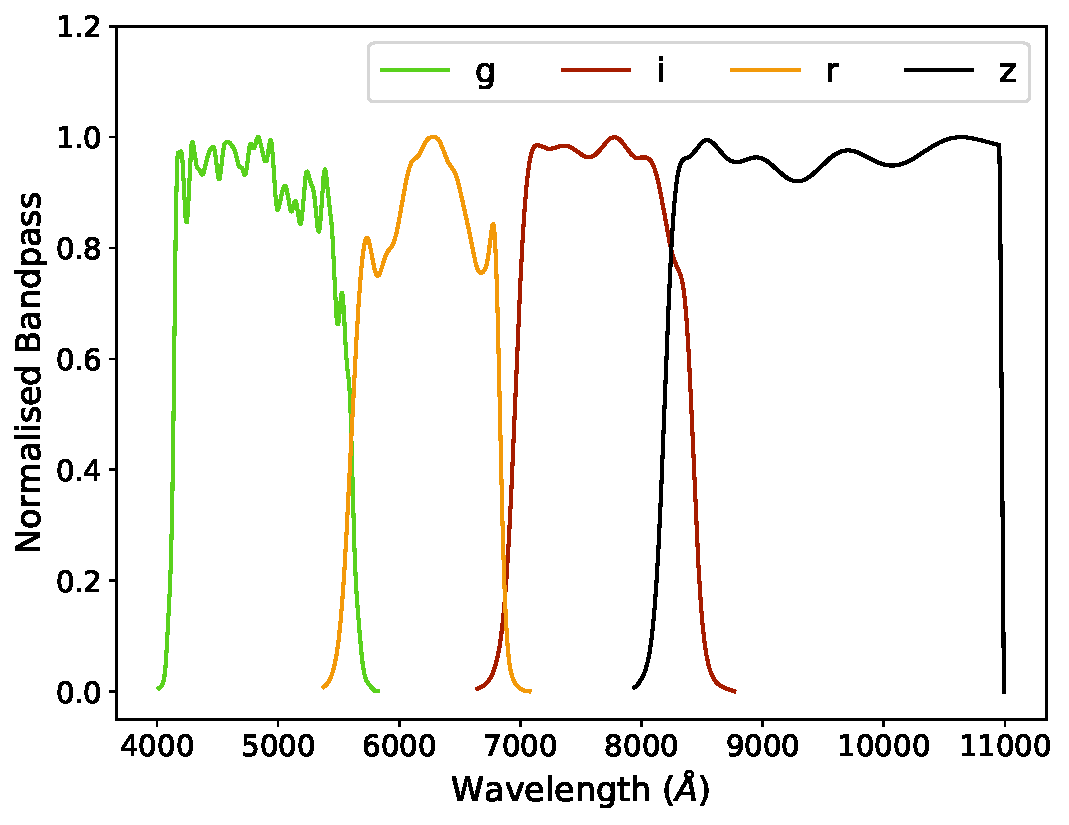
\includegraphics[scale=0.8]{Figures/Chapter2/SNLS_filters.pdf}
	\caption{Bandpass response for filters used in SNLS compared to a spectrum of a SLSN; SNLS06D4eu at z=1.588 discovered by the survey [TODO - PLOT AND BIN IT UP]}
    \label{fig:SNLSFilters}
\end{figure}

\subsection{Data Reduction}
Several different data reduction pipelines have been used in the analysis of the SNLS data. In this thesis, we used a combination of data prepared for public and internal data releases, we have also reanalysis the data for some objects of interest using PTFPhot, a custom, pre-existing pipeline designed to improve the data reduction quality for faint sources \citep{Firth2015}.

\subsubsection{Real-time photometry}
During the live operations of the survey, the data was pre-processed by applying flats and biases using the \textsc{Elixir} pipeline \citep{Magnier2004}. The data has then been independently analysed by the French and Canadian teams using separate quick-reduction pipelines \citep{Astier2006,Bazin2011}. Both teams aimed to produce lists of new, viable SN candidates within hours of their observations before sending them to the spectroscopic follow-up facilities. Both teams were very successful and produced mostly identical lists which lead to high classification accuracy, largely contributing to the overall success of the survey \citep{Pritchet2004}.

\subsubsection{Forced photometry}
The quick reduction pipelines used in the detection of objects were optimized with speed, as opposed to accuracy, in mind. Any scientific analysis of the data requires a more precise treatment of the photometry. The data for 'real' transient, defined as as having detections on multiple epochs and in multiple bands, was passed through an early version of PTFPhot \citep{Firth2015}, a much improved, custom, forced photometry pipeline. The improvements in the photometry, compared to the quick photometry, come mainly from the treatment of the PSF of the images. The quality of the science images is measured precisely on a number of stars, allowing for the reference images, usually with better quality, to be downgraded to match the quality of the science frames by convolving them with the PSF. Furthermore, the photometry is measured at the centroid for the source determined in a stack of all images as opposed to individual frames, giving rise to the term 'forced' photometry as the positions of the objects are forced to be consistent between all images. The full treatment of the PSF largely decreases the uncertainties associated with the flux measurement, especially for faint sources close to, or below, the detection limit. This analysis has been applied to the data releases that provided the sources and light curves for the work described in \cref{Chapter3} in similar way to other SNLS analysis such as the rates of SN-Ia \citep{Perrett2012} and core-collapse SN \citep{Bazin2009}, as well as the cosmological measurements \citep{Astier2006,Sullivan2011}.

\subsection{Spectroscopic Follow-Up}
The success of SNLS cannot be attributed only to the the number of transients discovered by the survey, but also to the effort behind the spectroscopic follow-up of the candidates. Between the Very Large Telescope (VLT), Keck, Gemini North and South and Magellan, more time has been allocated for spectroscopic follow-up than the time allocated to the photometric survey alone \citep{Pritchet2004}. As a result, 322 SN-Ia have been spectroscopically confirmed along with 51 CCSN and two SLSNe \citep{Guy2010,Howell2005,Howell2013}. A large number of the SN confirmed by the survey have been classified before or at their maximum thanks to both the follow-up selection criteria, which correctly identified the most promising candidates \citep{Sullivan2006}, and the readiness of the survey to sacrifice the classification rate in order to improve the quality of the data. While a large number of CCSN and AGN have been targeted for follow-up, which perhaps in the eyes of the primary goal of SNLS could be considered as undesired contaminants, this process also lead to the accidental discovery of two high redshift SLSN. These objects would be almost certainly overlooked if they were targeted post peak as their evolution would have strongly disfavored them as SN-Ia candidates. In turn, the rapid follow-up of SNLS06D4eu has produced a spectrum at a rest-frame phase of -34 days, which remains to this day as one of the earliest spectrum of a SLSN.

\subsection{Redshift measurements}
Distance measurements are invaluable in any type of SN analysis beyond just their application in cosmology. SNLS has provided three types of redshift measurements, used as distance probes: SN spectroscopic redshift, host galaxy spectroscopic redshift and photometric redshift estimates. The case of the SN spectroscopic redshift is the most accurate and rarely disputable as lines used to identify the redshift can be confirmed in the raw spectrographic images to be coincidental with the trace of the SN light. In SNLS this was measured for all classified SN. Furthermore, it may sometimes be possible to measure the redshift of an object that has an ambiguous classification as the some spectral features may be strong enough to be detectable despite low S\/N of the continuum.

Similarly to the SN spectroscopy, the host spectroscopy can provide a very high accuracy measurement of the redshift using narrow spectral features. However, it is possible that the host of the object may be misidentified. For example, the redshift might be measured for a bright galaxy apparently coincidental with the SN while the true host was a background galaxy or a dwarf foreground galaxy. Since these errors are relatively rare, we use both the target and host spectroscopic redshifts as absolute. SNLS, similarly to other large SN surveys, was not able to target all potential SN candidates during the live operations of the survey with many unclassified objects, later photometrically selected as good SN candidates after they faded below detection limit. \citet{Lidman2012} used the AAOmega multi fiber spectrograph on the Anglo-Australian Telescope (AAT) to target nearly 700 hosts of SN candidates in two of the four SNLS fields, obtaining redshift for 400 of them.

Beyond the spectroscopic measurement, it is also possible to estimate the redshift using the photometry of the galaxies. The SED of a galaxy usually contains a characteristic sharp break at $\sim$4000\AA which can be observed to transition between filters as the a function of redshift. This is a very powerful technique which, when used with a number of photometric filters, can very accurately estimate the redshift of a galaxy for $z$>0.3. Below that threshold, the SED break is contained within a single filter largely increasing the uncertainty of the estimate \citep{Connolly1995}. This technique has been used to estimate redshifts for over 500,000 galaxies within the CFHTLS, which overlapped with the SNLS fields giving a redshift estimate to nearly all candidates with a detected host \citep{Ilbert2006}.

\subsection{SLSN in SNLS}
As a survey designed with a heavy focus on SN-Ia, SNLS was not an ideal for detecting SLSN or other transients with relatively peculiar evolution. Its small area and relatively dense cadence meant that the volume searched was not sufficient to the detect a large number of SLSN, known to be a very rare class of astronomical events \citep{Cooke2012,Prajs2016,Quimby2013}. It is therefore perhaps not a coincidence that the only two objects detected by the survey were found at $z$=1.50 and $z$=1.588 where the survey was searching a much greater volume.

Beyond the nominal, live survey, the images for individual SNLS seasons have been co-added together to create "super" stacks, reaching a detection magnitude of $m$=26.5 \citep{Cooke2012}. A further two SLSN candidates have been detected using this technique. Their light curve behaviors were similar to that of a SLSN in terms of the absolute luminosity and temporal evolution. While it was impossible at that point (several years after the explosion time of the SN) to spectroscopically identify these objects, host galaxy spectroscopy was obtained for both objects determining redshifts of $z$=2.05 and $z$=3.9 \citep{Cooke2012}, confirming that these transients had a luminosities comparable to that of SLSN. While these candidate SLSNe show an interesting precedent for what may be hiding beyond the reach of our current 4m telescope class optical surveys, they were not used in any projects within this thesis. The lack of certain confirmation, low cadence in the stacked images light curve and the difference in the detection technique used deemed these objects incompatible with other SLSN data sources \citep{Prajs2016}.

\section{Dark Energy Survey}
The Dark Energy Survey (DES) is the largest cosmology survey operated to date. It is composed of two elements; a wide galaxy survey and a SN component. It's main aim is to perform the most precise to date measurement of the cosmological parameters. Many features and components of DES have been borrowed and improved on from previous surveys including SDSS and SNLS.

\subsection{Survey Setup}
DES uses a purpose build, 570 mega-pixel DECam CCD camera \citep{Honscheid2008,Flaugher2015} mounted on the 4m Blanco telescope at the Cerro-Tollolo observatory in Chile. One of the greatest advantages of DECam over its predecessors is its high sensitivity at red wavelengths allowing for high signal to noise observations in \textit{z} and \textit{y} bands compared to other surveys and allowing for SN detections at high redshift [INSERT FILTER PLOT]. DES was awarded 500 observing nights over the period of 5 years between 2013 and 2018 \citep{DES2016}. While the SN component has come to an end at the end of the fifth season as originally planned, the DES wide field component has been awarded more time to make up for the time lost due to unusually bad weather conditions in Chile over the last few years. Each season of observations started in late August and continued through to the end of January giving an average length of 5 months.

\subsubsection{Wide Survey}
DES wide survey has been designed to observe 5000 deg$^2$ of the southern sky to the depth of m$\sim$25 in the \textit{ugrizy} filters. The aim of this is to create the largest catalog of galaxies and their associated redshifts to date at an unprecedented resolution and depth for a ground based survey, with the first public data release contained a catalog of 400 million galaxies from the initial 3 years of the survey \citep{DES2018}. These data can be used to study cosmology via three separate experiments; the Baryon Acoustic Oscillations (BYO), Galaxy Clustering and Weak Lensing \citep{DES2016,Prat2017,Drlica-Wagner2017,DES2017}.

\subsubsection{Supernova Survey}
The goal of the DES SN search is to produce the largest, homogeneous catalog of SN-Ia to date. To achieve this, 10 observing fields have been selected are observed in the \textit{griz} photometric bands. Eight of these fields are 'shallow' and observe to the depth of m=23.5 while two fields have been chosen to be 'deep' and observe to m=25. The number of deep and shallow fields was chosen such as to maximize the number of discovered SN-Ia while still allowing for a sufficient number of high redshift objects to be detected \citep{Bernstein2012}.

\subsubsection{The cadence of the DES}
DES is composed of multiple elements, all with different core scientific and cadence requirements. In order to provide a fair and unbiased data set an automated scheduling algorithm has been used to maximize the scientific output [NEED TO FIND CITATION]. The Weak Lensing experiment provides the strongest constrain to the scheduling process. As it requires the measurement of the shape and orientation of galaxies with maximum available precision, it forces the wide fields to be observed only in the best, sub 1'' seeing conditions. As nights with suboptimal observing conditions are not ideal for the wide survey, the SN fields are observed instead often leading to a relatively dense cadence of low quality images in cases of persistent bad weather. This is most common at the start of every season when the observation take place in Chilean Winter/Spring. As the weather improves towards the Summer months, the seeing is rarely bad enough to give preference to the SN fields. To prevent the cadence from becoming too long the field are observed on a "dead man" trigger after 7 nights without observations, regardless of the conditions.

\subsection{Data Reduction}
While the basic structure and principles behind the data reduction in DES is very similar to that of SNLS, the major differences lay in the treatment of transient detection in the difference images. As the volume of data in DES was too large to allow for manual selection of real sources as a long term solution. Manual classification was performed only in the first year of the survey operation. This dataset was then used as a training sample for machine learning classification pipeline, \textsc{autoScan} \cite{Goldstein2015}.

Thanks to a large amount of computing resources available to the survey the computationally expensive force photometry has been automatically performed on every transient candidate, defines as an object with at least three detections in a minimum of two different bands where the detections were within 30 days but not all on the same night.

Further to Force Photometry, DES has recently developed a Scene Modeling Photometry (SMP) pipeline for use with the SN data. SMP can greatly reduce the uncertainties associated with transient photometry by removing the requirement for template images. Instead of subtracting a downgraded in quality template from a science frames, the pixels in the region surrounding a transient are modeled individually as constant values with a variable source placed over them. The models are then processed to match the quality of the images before they are ingested into a fitting routine. While this technique provides data with superior quality it was introduced into the survey at a very late stage of this thesis making it impossible to be implemented.

\subsection{Spectroscopic redshift}
One of the biggest differences in the design of DES versus other SNIa surveys is its approach to redshift measurements.

\subsubsection{Host galaxy redshift}
From the predicted number of objects to be detected by DES it was clear, since the early planning stages, that it would be impossible to obtain spectroscopic redshift using the SN spectra for all the candidates. The survey therefore focused on obtaining the spectroscopic redshift of the host galaxy for all objects. This is being achieved in collaboration with OzDES, an Australian survey using the AAOmega multi-fiber spectrograph mounted on the AAT telescope dedicated to spectroscopic follow-up of DES SN fields. All real transients are targeted regardless of the brightness of their host as the target is observed multiple times over the duration of the survey and the spectra are stacked. Is some cases redshift has been measured in galaxies down to 24.5 magnitudes. Furthermore, DES SN fields were purposely selected to overlap with other surveys in order to provide a catalog of redshifts for galaxies in the fields. This included Chandra Deep Field South (CDF-S), European Large Area ISO Survey (ELAIS), XMM Large Scale Structure survey (XMM-LSS) as well as SNLS and the SDSS Stripe82 regions. 

\subsubsection{Hostless SN}
While redshifts for the majority of SNe can be obtain from their hosts, there remain some that are associated with galaxies fainter than the detection limit of even the stacked AAT spectra. For these objects it is critical that the redshifts are measured during the live transient which has been the main focus of the extensive spectroscopic campaign. A number of facilities including VLT, Keck, Magellan, MMT, SALT SOAR and NTT amongst others have been used, giving a total of XXX hours or observing time. xxx SNIa have been classifies along with xx CCSN and xx SLSNe. A short description and circumstances involving the classification of DES SLSN are described in \sref{sec:DES_SLSN} [ASK MAT FOR CHRIS'S PAPER TO FIX THESE]

\subsection{Photometric Redshifts}
All experiments that form part of DES rely heavily on photometric redshift measurements making it an integral part of the survey. The wide component uses the measurement as a base for their cosmological measurements as it is currently impossible to measure spectroscopic redshifts for even a fraction of the nearly half a billion galaxies detected by DES. The SN survey used the measurements as redshift priors in transient classification. These fits are not used for cosmology, instead they act as a prioritizing tool for the spectroscopic follow-up program. Photometric redshifts have also been used as part of the SLSN search. While most SLSNe would be expected to have a faint or no host associated with them, thanks to their common association with dwarf galaxies, we have used the photometric information (also the lack of it) as a possible sign that an object may be a SLSN, e.g. in cases where the galaxy was measured to be too local or where there was no photometric redshift present meaning that the object can be considered as 'hostless'. This is described in more details in \cref{Chapter5}. 

\subsection{SLSNe in DES}
\label{sec:DES_SLSN}
While SLSNe have never been a primary target of DES, their potential use as cosmological probes \citep{Inserra2014} meant that they have generated a large interest within the survey. The first SLSN, and the only one detected in the first season of the survey, DES13S2cmm has been classified using a Directors Discretionary Time (DTT) program at the VLT and was published as one of the earliest results from DES \cite{Papadopoulos2015}. In the following seasons the number of objects discovered has increased dramatically with $\sim$6 objects confirmed per year, giving motivation to the photometric search for the missing SLSN in the data performed in this thesis. The sample (Angus et al. in prep), has shown a large diversity between the objects with many falling outside of the 'classical' definition of a SLSN \citep{Inserra2018}. I briefly outline the spectroscopic sample from the first four years of DES and its properties as well as any peculiarities in the lightcurve or spectral evolution in context of their modeling and comparisons with the photometric sample of SLSN described in \cref{Chapter6}.   

[MARK: SHOULD THIS SECTION HAVE PLOTS OF ALL SLSNE FOUND IN DES OR SHOULD I PUT THIS IN THE APPENDIX]

\subsubsection{DES13S2cmm}
DES13S2cmm was the first SLSN discovered by DES. It was identified during a visual light curve scan and quickly selected as a potential SLSN candidate due to its particularly long rise and faint host. A spectrum of the SN has been obtained using the FORS2 instrument on the VLT using a DDT proposal. The observation confirmed that the SN is at z=0.609 and has features resembling other SLSNe. At the time of discovery this was one of the lowest luminosities SLSNe at M$_U$=-20.0.

\subsubsection{DES14C1fi}
This object was similarly identified manually as a plausible candidate thanks to its slow evolution. It was observed at the Keck telescope and again, 7 days later, using VLT's XShooter which found a featureless continuum that almost precisely matched a blackbody SED. A XXXXA oxygen absorption doublet was used to identify the redshift as z=1.40 giving it a luminosity of M$_U$ = -21.9. While the result is somewhat tentative due to a very low S\/N in the IR arm of XShooter, there is a possible sign of a broad H-alpha feature. DES14C1fi is the only SLSN in the DES Y1-4 sample that shows potential signs of being a SLSN-II candidate. 

\subsubsection{DES14C1rhg}
DES14C1rhg was targeted as a hostless SLSN candidate based on its long rise time of 30 days. It was observed using our XShooter SLSN program and confirmed at z=0.47 putting it a lower than expected redshift for a SLSN of that apparent magnitude and giving it a luminosity of M$_U$ = -19.2. Combining its low brightness with a relatively fast decline time puts DES14C1rhg on the extreme of the population making it incompatible with any current photometric definition of a SLSN despite its spectroscopic resemblance. 

\subsubsection{DES14E2slp}
DES14E2slp was detected at a very late stage of the season with only a single epoch of observations after maximum light. It was selected as a target for the VLT/XShooter program due to being blue, hostless and relatively slowly rising. The classification spectrum was taken at a phase of $\sim$-20days and showed a blue, featureless continuum despite a relatively high S\/N. A spectroscopic redshift was measured using a weak absorption feature to be z=0.64 placing giving the object a luminosity of M$_U$ = -20.5. With the inconclusive spectroscopic redshift, no decline data and no spectral features this remains as the most tentatively confirmed SLSN in our sample.

\subsubsection{DES14S2qri}
DES14S2qri is the most peculiar SLSN detected in the second season of DES. It was targeted for follow-up as a hostless object with a long rise in the redder bands. Its spectrum perfectly matches that of a SLSN at z=1.5 making it the highest redshift SN found up to that point of the survey. More interestingly, it featured some of the most unusual behaviours in the observer frame g-band where the object is not detected until the maximum light. Magnetar modeling of the light curve shows that the g-band underwent very strong absorption in the early stages before returning to the expected SED. Unfortunately the classification spectrum was taken too late to observe this behaviour.

\subsubsection{DES14X2byo}
DES14X2byo is one of the bluest SLSNe ever discover, reaching a photospheric temperatures of 27,000K. Despite this it had a an average evolution and peak magnitude (for a SLSN) making its colour even more puzzling. One possible suggestion is that a pre-peak event like the one seen in DES14X3taz took place at the same time as the onset of the spin-down of the central engine injecting extra energy which thermalised to produce the excess temperature.     

\subsubsection{DES14X3taz}
DES14X3taz was the second SLSN published as part of DES and is one of the most important objects of this class seen to date as it is the most well observed example of a pre-maximum "bumps" in a SLSN. It was initially misidentifies as a potential SNIa during the "bump" phase but never targeted at that stage before, during a manual scan of the light curves, it was observed to be rising again. The spectrum taken pre-peak has confirmed the object to be a perfect match to a SLSN at z=0.608. Further discussion of the modeling of this object can be found in \cref{Chapter4} where we model this object using a combination of the Magnetar model and ejectra spreading inside of a dense, extended wind envelope \citep{Piro2015}.

\subsubsection{DES15C3hav}
In a sample full of what one could describe as peculiar SLSN, DES15C3hav stands out as one of the deepest mysteries the field has to offer. The object was discovered in the later stages of the third season of DES and was targeted as an early SNIa spectra program at the MMT. It was then identified as a SLSN at z=0.39 giving it a peak magnitude of M$_U$=-19.1 making it the least luminous example of its class. However, it wasn't until after the classification of the object that we discovered that the SN was associated with a pre-peak bump. While this would normally not been considered unusual for a SLSN, the bump was observed to have a peak luminosity of M$_U$=-16 which is nearly 3 magnitudes dimmer than any previous example of its class, it was relatively red with the peak temperature of 6,500K and is consistent with an explosion before the start of the season making its rise time longer than 50 days. These three characteristics are are nearly the exact opposite to what would be expected of a SLSN bump and also do not match any known type of transient known to us.

\subsubsection{DES15E2mlf}
a

\subsubsection{DES15S1nog}
b

\subsubsection{DES15S2nr}
c

\subsubsection{DES15X1noe}
d

\subsubsection{DES15X3hm}
e

\subsubsection{ADD MORE ... }
f

\section{SUDSS}
The Search Using DECam for Superluminous Supernovae (SUDSS) (PI: Sullivan) was designed as a dedicated SLSN survey working in conjunction with DES. Its aim was to extend the DES observing season from $\sim$6 months to $\sim$9 months by observing the fields, even at high airmass, until the observations become impossible due the sun constrains. The motivation behind the survey was the possibility of using SLSNe as a cosmological probe \citep{Inserra2014}. As this aligned well with the overall goal of its mother survey, SUDSS was awarded XX nights in between the end of DES Y1 and start of DES Y4. Unfortunately, due to issues with the data quality and reduction (see \sref{sec:SUDSSIssues}), it has never been used as a tool for searching for new SLSN candidates, partially leading to the support for the survey and telescope time being withdrawn before the end of DES operations. Regardless, SUDSS has greatly enhanced the light curves of some SLSNe discovered by DES and strongly contributed to the analysis of their sample.

\subsection{Observations and Data Reduction}
SUDSS observed XX fields with XX fields overlapping with DES, including [NAME]. XX fields were selected as stand alone field to allow for observations to take place when DES fields have already moved behind the sun. The observations were carried out using DECam with an identical setup to DES allowing for the same pre-processing steps to be applied to the data. The data was not directly fed into the DES database nor did it use the force photometry pipeline used by DES for technical reasons. Instead the data was reduced using a custom PTFPhot pipeline \citep{Firth2015}. For the purpose of unbiased comparison, corresponding DES observations of the SUDSS SLSNe were also reduced using the PTFPhot pipeline.

\subsection{Cadance and Exposures}
\label{sec:SUDSSCadance}
SUDSS was designed with the aim of discovering new SLSN candidates at its very heart. It was initially estimated that it will be capable of identifying $\sim$ 200 SLSN candidates during its operation \citep{Papadopoulos2015}. As SLSN are a class of slowly evolving supernova, the DES observing cadence was not replicated for SUDSS and instead it was chosen to be approximately two weeks. Due to worse that anticipated weather conditions, many of these nights have been lost to clouds resulting in a final cadence closer to approximately a month. On average three additional observations were made in each field outside of the DES observing season.

A further difference between the DES and SUDSS observing strategies comes in the exposure times used for the observations. As SLSN are much brighter but rarer events than SNIa the exposure times did not have to match that of the DES deep fields. The exposure times are in between that of the DES shallow and deep fields allowing for a balance between the number of observed fields and the volume searched that is optimized for SLSN. In practice, the limiting magnitude of SUDSS was similar to that of the DES shallow fields once the unfavorable atmospheric conditions and high air mass have been taken into account.

\subsection{Spectroscopic Follow-up}
As SUDSS operated outside of the DES, we could not rely on the DES spectroscopic follow-up campaign to classify newly discovered SLSNe. For this purpose we have been awarded XX hours on the VLT's XSHOOTER instrument in program PXX. As the survey did not provide any new candidates for classification, the time has been used to follow-up candidates that were identifies in DES and visible in the SUDSS fields. [CHECK WHICH SN HAVE BEEN CLASSIFIED USING THAT PROGRAM] 

\subsection{Findings}
\label{sec:SUDSSIssues}
As a result of the poor cadence and lower than expected image quality it was not possible to carry out a dedicated search for SLSN in the SUDSS data alone. Instead, the SUDSS data has been re-purposed as an auxiliary data source for objects already discovered by DES. This has been extremely successful and resulted in a great improvement to the light curves of some of the SLSNe discover by DES. In cases of DES15C3hav and DES15X2hm we were able to determine the explosion date and hence constrain the rise time of these SNe using the SUDSS data points.

The most significant observations came in form of DES14X3taz where the auxiliary SUDSS data provided the observations of the pivotal rise and peak of this unique "bumpy" SLSN. Without the SUDSS observations a large proportion of the analysis carried out in \citep{Smith2016} would have not been possible.

\section{Literature sample of SLSNe}
As SLSNe are still a new and rapidly evolving branch of SN research, they definition has been a subject to debate since their first discovery \citep{Gal-Yam2012,Inserra2013,Nicholl2014}. Recently proposed classification method by \citet{Inserra2018}, which involves measuring the peak and colour of the SLSN at peak and 30 days post maximum light, was not available at the time when all projects described in this thesis were undertaken. While the new approach has been used in the DES Machine Learning classification study \cref{Chapter5}, the measurement of the rate of SLSNe in SNLS was done using our own definition described in \cref{Chapter3}. Any attempt of defining a class requires a training sample of examples that inform that definition. 

In this thesis we have collected the data for large number of literature SLSNe data, published in years between 2010 and 2016, including their light curves and spectra. This was not limited to object published in journals but also included Astronomical Telegrams (ATels) as well as spectra published on the online WISeREP repository \citep{Yaron2012}. producing a list similar to that published recently by \citet{Schulze2017}. It is important to note at this point that in this work we were only interested in hydrogen poor SLSN, however, we did not distinguish between slowly and rapidly evolving objects \citep{Gal-Yam2012,Inserra2013}. 

\subsection{Quality cuts}
Many of the object in this list were of very poor quality containing only either a handful of photometric points and single classification spectra with no data for their evolution. Furthermore the data originated from a variety of sources including PTF, iPTF, SNLS, DES, Pan-STARRS and LSQ amongst others, giving a broad range of photometric bands and systems.

We devised a set of quality cuts to ensure that the objects used in our analysis meet a minimum standard. As most of our analysis, discussed in the forthcoming chapters, depends on fitting black bodies to the data, we require that the light curve must contain a minimum of three distinct photometric bands. While in the later modeling we treat such bands independently, for the purpose of the quality cuts we take bands that are derivatives of each other (i.e R and r) as the same. Furthermore we make cuts based on the number of epochs observed per band. In order to use models which depend on the rise and decline time of the supernova we require that there are a minimum of two photometric points before the maximum light and two points after the peak. As the SN evolve rapidly in temperature (and hence colour) the bluer bands peak several days before redder bands. We define the peak as the maximum in the band closest to rest frame U-band. \tref{tab:PubishedSLSNe} shows the final list of SLSN, available at the time, that passed our data quality cuts and have hence been used in \cref{Chapter3} as the base for our definition of SLSNe.

\subsection{Converting and converging photometric systems}
It is standard practice in the SN literature to publish the photometry for studied objects in form of a table of magnitudes per band on given observing nights. Magnitude scale is not however optimal when fitting models to the data. As it is logarithmic in nature, the photometric uncertainties, originally measured in the linear count space and Gaussian in nature become asymmetric and therefore more difficult to deal with in model fitting. It is easier to simply convert the magnitudes, M, to flux, $\nu$ using a zero point, $zp$ for a given filter:

\begin{equation}
\label{eq:MagToFlux}
\nu = 10^{-0.4 \times M~+~zp}
\end{equation}

similarly we convert the uncertainties in magnitude to flux using \eqref{eq:MagErrorToFlux}.

\begin{equation}
\label{eq:MagErrorToFlux}
\Delta \nu = 0.921034~\times~10^{-0.4 \times M~+~zp}~\times~\Delta M
\end{equation}

It is customary in literature to quote the magnitudes for the SDSS-like filters (\textit{ugrizy}) in the AB photometric system and the Johnson filters (\textit{UBVRIJHK}) in the Vega system. If not otherwise stated in the papers, these are the systems used for the zero points in conversion between magnitude and flux. If not stated otherwise it is also assumed that the photometry has been corrected for Milky Way extinction which is a standard procedure in most modern surveys [CITE PTF, DES, SNLS etc].

\begin{table}
\begin{center}
  \caption{The training sample of SLSNe-I.}
\label{tab:PubishedSLSNe}
\begin{tabular}{|l|r|l|l|}
\hline
  \multicolumn{1}{|c|}{SN Name} &
  \multicolumn{1}{c|}{Redshift} &
  \multicolumn{1}{c|}{Survey} &
  \multicolumn{1}{c|}{Reference} \\
\hline
  PTF12dam & 0.108 & Palomar Transient Factory & \citet{Nicholl2013}\\
  SN2011ke & 0.143 & Catalina Real-Time Transient Survey & \citet{Inserra2013}\\
  &&\& Palomar Transient Factor & \\
  SN2012il & 0.175 & Pan-STARRS & \citet{Lunnan2013}\\
  SN2010gx & 0.230 & Palomar Transient Factory & \citet{Pastorello2010}\\
  PTF09cnd & 0.258 & Palomar Transient Factory & \citet{Quimby2011}\\
  SN2013dg & 0.265 & Catalina Real-Time Transient Survey & \citet{Nicholl2014} \\
  PS1-11ap & 0.524 & Pan-STARRS & \citet{McCrum2014a}\\
  DES14X3taz & 0.608 & Dark Energy Survey & \citet{Smith2016} \\
  PS1-10bzj & 0.650 & Pan-STARRS & \citet{Lunnan2013}\\
  DES13S2cmm & 0.663 & Dark Energy Survey & \citet{Papadopoulos2015} \\
  iPTF13ajg & 0.741 & intermediate Palomar Transient Factory &\citet{Vreeswijk2014}\\
  PS1-10awh & 0.909 & Pan-STARRS & \citet{Chomiuk2011}\\
  SNLS-07D2bv & 1.500 & Supernova Legacy Survey &\citet{Howell2013}\\
  SNLS-06D4eu & 1.588 & Supernova Legacy Survey &\citet{Howell2013}\\
\hline\end{tabular}
\end{center}
\end{table}
 % Background Theory 

%\chapter{Rate of SLSNe at z$\sim$1}
\label{Chapter3}
\lhead{Chapter 3. \emph{Rate of SLSNe}}

The rate of any transient event is one of its most fundamental properties, providing clues about their origin and evolution throughout the history of the universe. In this chapter I present the measurement of a volumetric rate of SLSNe at z$\sim$1 measured using the archival SNLS data, providing a unique opportunity to test their progenitor models. Since their identification, SLSNe have been known to be an extremely rare class of events. The low rate suggests that the origin of SLSNe must be connected with an equally rare progenitor scenario. The motivation behind our measuring is to study the evolution of the rate by bridging the gap between the local and high redshift measurements of the rate.

Prior to this work, there were three published measurements of the rate of SLSNe. A local rate of was calculated using a single SLSN-I event discovered by the Texas Supernova Search (TSS) \citep{Quimby2014}, giving a value of $\rho_{\mathrm{SLSN}} = 19^{73}_{17}$ SNe Gpc$^{-3}$ Yr$^{-1}$ at the volume weighted redshift of z=0.23. The large measurement uncertainty can be attributed to the Poissonian statistics of their scarce sample as well as the uncertainty in the detection efficiency driven by the diversity of SLSN population. In contrast to the local value, \citet{Cookie2013} presented a rate of SLSNe at a volume-weighted z$\sim$3 using two SLSNe discovered in the deep stacked SNLS data. They estimate $\rho_{\mathrm{SLSN}}$ = 400 SNe Gpc$^{-3}$ Yr$^{-1}$, however, do not provide an uncertainty estimate which we must assume, making a conservative estimate to be 50\%. The final of the three measurements was performed by \citet{McCrum2015} using a sample of spectroscopically confirmed SLSNe in the PanSTARRS. This measurement, however, used a different approach basing the rate of SLSNe on the relative rate and spectroscopic completeness with respect to CCSNe discovered in the same data set. While I include this measurement for comparison purposes, the values cannot be directly related.

None of the above experiments measures the rate in the region of z$\sim$1, leading to a gap near to the peak of the star formation history of the universe. This region is particularly interesting to us, not only as there is a large number of SLSNe detected at that redshift, but also as a test for a number of progenitor theories. The rate measured in that volume is fundamental in order to establish whether the rate of SLSNe follows that of the star formation history of the Universe. Demonstrating this could give further evidence to support the models where the birth of a SLSN is connected to a death of a very massive and therefore young progenitor.

SNLS provides a great dataset for this project. With detecting high redshift SNIa as one of its main goals, the SNLS dataset is full of deep and high-quality light curves. The survey has already serendipitously discovered two, high redshift, SLSN \citep{Howell2013} making it a safe choice while simultaneously having a potential to hide more, not yet identified objects. This work follows a series of similar measurements performed using the same dataset. The rate of SNIa, as well as the point source detection efficiencies, were found by \citet{Perrett2012}. The rate of CCSN was measured by \citet{Bazin2009}, providing a unique opportunity to compare the rate of SLSNe and CCSN using a deep, homogeneous dataset.

The order of this chapter is as follows. First, I propose a photometric definition of SLSNe based on the modelling of their light curves using the spin-down of a magnetar model followed by a search for missed objects within the SNLS dataset. I briefly introduce the photometric sample of SNLS SLSNe before describing the Monte Carlo simulation used in order to measure the rate and its uncertainties. Finally, I compare the value measured to the previously published results and discuss its significance in terms of the physical origin of the objects as well as their detectability by DES and future surveys. The work presented in this chapter has been published in \citet{Prajs2016}.

\section{Defining a SLSN}
\label{sec:SLSNDefinition}
The first task in the process of measuring the rate of SLSNe was to develop a method for the photometric selection of optical transients that were to enter our SLSN sample. The earliest definitions of SLSNe relied on their peak luminosity and often defined them as SN with an absolute $u$-band magnitude of $M_{u}<-21$ \citep{Gal-Yam2012}. This definition is not adequate for our search for two main reasons. Firstly, after that definition was formulated, several examples of events that are spectroscopically similar to SLSNe but that do not pass this arbitrary threshold have been discovered. Some of these events included DES13S2cmm \citep{Papadopoulos2015} and LSQ14mo \citep{Leloudas2015a} which both have M$_u$ > -21 despite being spectroscopically consistant with SLSNe and are associated with a very slow light curve evolution. Secondly, a new class of fast and luminous transients with luminosities similar to SLSNe but with a faster light curve evolution as well as different spectroscopic types, has recently been discovered \citep{Arcavi2016}. Instead of an arbitrary luminosity cut, I use a photometric classification approach based on the modeling of SLSNe using the spin-down of a magnetar model as a simple analytical model that provides a good fit to a sample of confirmed SLSNe.

As an early approach to the problem of classifying SLSNe, this approach did have several drawbacks. The use of an analytical model implied that the rate was calculated only for objects which are similar to the sample of confirmed SLSNe, as presented in \sref{sec:litSample}. It was clear, at the time this work was undertaken, that this would likely not capture all objects of this class. Without a better definition of a SLSN more significant progress could not be achieved. In \cref{Chapter5} I present a more sophisticated and complex approach to this problem, based on an artificial training sample of SLSNe and Machine Learning classifiers, before applying it to DES.

\subsection{Modeling SLSNe}
In order to model SLSN I required two main ingredients: an underlying model for the time-dependent bolometric luminosity of a SLSN, and an SED that can convert this bolometric luminosity into time-evolving spectra. This together forms a spectral series from which we can synthesis the photometry in any desired filter and at any desired redshift. This can then be used for comparison to observed data. For the purpose of this chapter the exact form or the physical meaning behind the light curve model parameters are irrelevant as, in practice, any model that satisfactorily replicates the observables could be used for this purpose. I therefore provide only a brief overview of the model here while the remaining details are described in \sref{sec:SLAP}.

\subsubsection{Magnetar model}
The spin-down of a magnetar model assumes that a collapse of a giant star with an initial mass of M $>$ 40M$_{\odot}$ produces a SNIc like explosion whilst giving birth to a magnetar; a highly magnetized neutron star with a rotation period on the time scale of milliseconds \citep{Kasen2009,Woosley2010,Inserra2013}. The simple toy model assumes a spherically symmetric ejecta and a constant opacity. The free parameters in the model are the time of explosion, $t_{\mathrm{expl}}$, the magnetic field, $B_{14}$, spin period, $P_{\mathrm{ms}}$ and the diffusion timescale $\tau_M$ which is directly proportional to the ejecta mass, M$_{\mathrm{ej}}$.

\subsubsection{Fitting literature light curves}
The magnetar model provides a good fit to all the SLSNe that form part of our training sample. \tref{table:Magnetar} contains the model's best-fit parameters, as well as two additional derived observables which help us to identify the nature of the events without visually inspecting the light curves. These are the peak absolute magnitude in the SDSS $u$-band filter as well as the rise-time, $t_\mathrm{rise}$, of the SN as measured from explosion to maximum light in the rest-frame $u$-band. It is important to note here that the absolute magnitude, $M_u$, are given in the AB magnitude system. The zero-point correction factor betwee the AB and Vega magnitude system for the $u$-band filter is: $M_u^{\mathrm{AB}}\simeq M_u^{\mathrm{vega}}+0.9$ \citep{2007AJ....133..734B}. Therefore, while some of the training sample have $M_u^{\mathrm{AB}}>-21$, none have $M_u^{\mathrm{vega}}>-21$ which agrees with the previous definition of a SLSN.

\begin{table}
\begin{center}
\caption{Magnetar model parameters for the sample of 15 published SLSNe.}
\label{table:Magnetar}
\begin{tabular}{|l|r|r|r|r|r|r|r|r|r|r|}
\hline
  \multicolumn{1}{|c|}{Name} &
  \multicolumn{1}{c|}{$M_u$} &
  \multicolumn{1}{c|}{$t_\mathrm{rise}$} &
  \multicolumn{1}{c|}{$\tau_\mathrm{m}$} &
  \multicolumn{1}{c|}{$B_{14}$} &
  \multicolumn{1}{c|}{$P_{\mathrm{ms}}$} &
  \multicolumn{1}{c|}{$t_\mathrm{expl}$} &
  \multicolumn{1}{c|}{$E(B-V)$} &
  \multicolumn{1}{c|}{$\chi^2_{\nu}$} &
  \multicolumn{1}{c|}{Template} \\ & &
  \multicolumn{1}{c|}{(days)} &
  \multicolumn{1}{c|}{(days)} &
  \multicolumn{1}{c|}{($\times10^{14}$ G)} &
  \multicolumn{1}{c|}{(ms)} &
  \multicolumn{1}{c|}{(MJD)} & \\
\hline
  PTF12dam & -21.4 & 34.72 & 22.15 & 0.78 & 2.85 & 56044.5 & 0.18 & 2.49 & 06D4eu\\
  SN2011ke & -21.2 & 24.84 & 30.61 & 3.67 & 2.13 & 55647.5 & 0.01 & 1.31 & iPTF13ajg\\
  SN2010gx & -21.7 & 24.56 & 30.36 & 3.20 & 1.54 & 55247.1 & 0.19 & 0.86 & 06D4eu\\
  SN2013dg & -21.2 & 25.37 & 28.05 & 3.30 & 2.75 & 56412.3 & 0.07 & 0.23 & SCP06F6\\
  PS1-11ap & -21.8 & 32.1 & 20.08 & 0.79 & 2.51 & 55559.0 & 0.02 & 1.62 & 06D4eu\\
  DES14X3taz & -21.7 & 47.21 & 26.16 & 0.23 & 1.67 & 57019.2 & 0.09 & 5.18 & 06D4eu\\
  PS1-10bzj & -21.2 & 22.17 & 18.44 & 2.65 & 3.84 & 55524.0 & 0.07 & 0.37 & 06D4eu\\
  DES13S2cmm & -20.0 & 30.7 & 21.19 & 1.28 & 5.29 & 56509.0 & 0.01 & 0.51 & 06D4eu\\
  iPTF13ajg & -22.4 & 31.45 & 33.41 & 1.57 & 1.32 & 56346.9 & 0.19 & 0.30 & iPTF13ajg\\
  07D2bv & -21.1 & 28.41 & 36.88 & 3.40 & 2.18 & 54132.4 & 0.05 & 0.41 & SCP06F6\\
  06D4eu & -21.9 & 21.48 & 29.94 & 3.82 & 1.00 & 53956.3 & 0.11 & 1.26 & 06D4eu\\
\hline\end{tabular}
\end{center}
\end{table}

\subsubsection{Defing a SLSN parameter space}
\fref{fig:SLAPparam} shows the best-fit magnetar model parameter space. In order to define a region of the parameter space that defines a SLSN I enclosed the cluster of our literature points with an ellipsoid. I chose it as the lowest volume, simple geometric body that was consistent with all the SLSN in our training sample. The ellipsoid is defined in terms of the three main fit parameters of the magnetar model, $\tau_\mathrm{m}$, $B_{14}$ and $P_{\mathrm{ms}}$. In the Cartesian coordinate system a position on any generic ellipsoid can be defined using \eref{eq:Ellipsoid}.

\begin{equation}
\label{eq:Ellipsoid}
\left( \begin{matrix}
x \\
y \\
z
\end{matrix} \right)
=
\mathbf{A}
\left( \begin{matrix}
R_x\cos(u)\cos(v) \\
R_y\cos(u)\sin(v) \\
R_z\cos(v)
\end{matrix} \right)
+ \mathbf{C}
\end{equation}

\noindent where \textbf{A} is a rotation matrix, \textbf{R} is the radius of the ellipsoid and \textbf{C} is the position of its center. The following conditions must be satisfied: $-\pi /2 \leq u \leq \pi /2$ and $-\pi \leq v \leq \pi$. I have set up our parameter space such that $\tau_\mathrm{m}$ lays along the $x$-axis, $B_{14}$ is along the $y$-axis and $P_{\mathrm{ms}}$ corresponding to the $z$-axis. Using the Khachiyan Algorithm \citep{Aspvall19801,KHACHIYAN198053}, I performed an analytical fit to determine the ellipsoid that best describes the known population of SLSNe. I found the best-fit ellipsoid to have the following properties:

\begin{equation}
\label{eq:A}
\mathbf{A} =
\left( \begin{matrix}
-0.184 & 0.575 & -0.797\\
 0.008 & 0.812 & 0.586\\
0.983 & 0.102 & -0.154
\end{matrix} \right)
\end{equation}

\begin{equation}
\label{eq:R}
\mathbf{R} =
\left( \begin{matrix}
R_x \\
R_y \\
R_z
\end{matrix} \right)
=
\left( \begin{matrix}
1.89\\
2.17\\
11.32
\end{matrix} \right)
\end{equation}

\begin{equation}
\label{eq:C}
\mathbf{C} =
\left( \begin{matrix}
26.76 \\
2.14\\
2.77
\end{matrix} \right)
\end{equation}

\noindent \fref{fig:SLAPparam} shows the three, two-dimensional projections of this parameter space, populated with our training sample of literature SLSNe.

\begin{figure}
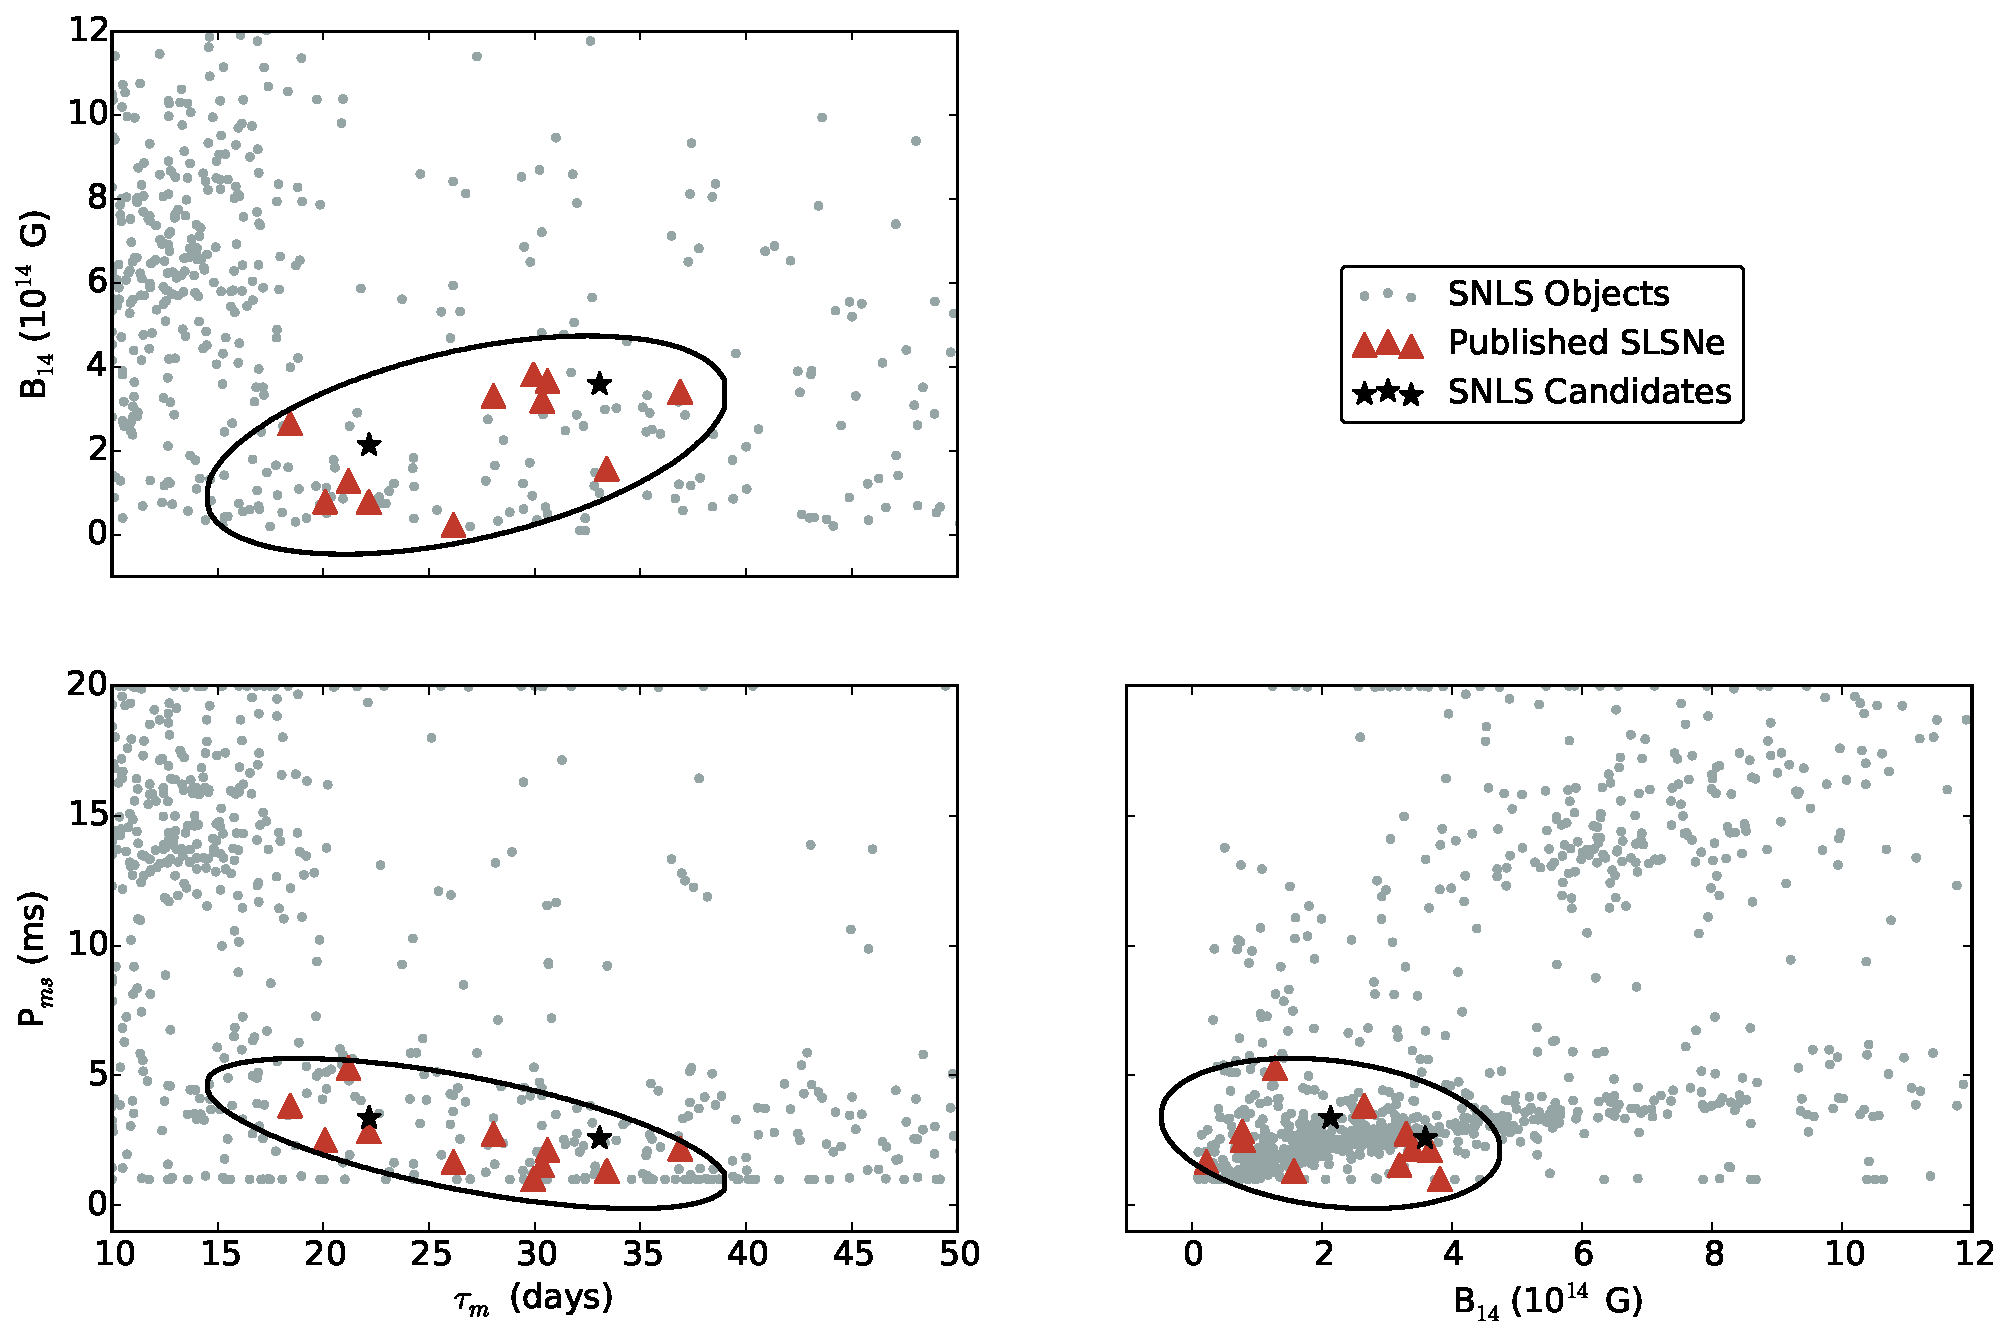
\includegraphics[width=\textwidth]{Figures/Chapter3/SLAPparam}
\caption{The $\tau_\mathrm{m}$--$B_{14}$--$P_{\mathrm{ms}}$ parameter space constructed from the magnetar model fits. The SNLS objects are denoted by grey circles. The ellipses correspond to the two dimensional projections of the three dimensional ellipsoid, fitted around the parameter space of the known SLSNe (shown as triangles) to form a region defining them in terms of the model. The SNLS candidates that fall within this parameter space are shown as stars.}
\label{fig:SLAPparam}
\end{figure}

\section{Searching for SLSN in SNLS}
Having formed a photometric definition of SLSNe in \sref{sec:SLSNDefinition} I now proceed to describe the steps undertaken in order to identify any potential missed SLSNe in SNLS. My approach was based on fitting the magnetar model to SNLS light curves and comparing their best-fits to the parameter space defined by the training sample. In the ideal case we would first like to test the definition against an independent test sample of objects that were not used in forming the definition. Unfortunately, the number of known SLSN events at that time was so low that we could not afford to split it into a training and test samples. I therefore make the assumption that the parameter space in \fref{fig:SLAPparam} is defined by a representative sample of events. This privides a further motived to seek a more elegant and robust solution for any future search of SLSN such as the one performed on the DES dataset in \cref{Chapter5}. I would also like to note that both the fitting method and the definition of a SLSN-like event presented in this chapter do not makes any assumption about the luminosity of the event. This makes it entirelly possible for fitted events to have $M_u>-21$ and still be classified as SLSNe, therefore broadening the current definition of SLSN into potentially previously unexplored parts of the parameter space. The invervse is also true, where some events with $M_u<-21$, including those with a relatively short diffusion timescale, $\tau_\mathrm{m}$, giving rise to a faster evolution, are shown to be inconsistent with SLSNe. This natural consequence of the technique used here is should therefore lead to a purer sample of SLSNe than a arbitrary magnitude cut.

\subsection{Magnetar model fitting}
With the model and definition of SLSNe in place, my next task was to apply the same technique to the sample of SNLS transients. The SNLS detected 4949 transient objects in total \citep{Perrett2010}. This included many objects that were visually designated as active galactic nuclei (AGN) and variable stars, as well as supernovae. In order to perform the fitting on the sample I first matched each object with a redshift where known. 1694 object in the transient catalogue have spectroscopic redshifts, either from spectra of the transients or of the host galaxy.

As previously described in \sref{sec:SNLSRedshift}, where a spectroscopic redshift is not available, I use photometric redshift estimates. SNLS transients were associated with potential host galaxies by selecting the nearest galaxy within a radius of 1.5''. This provided photometric redshift information for a further 1527 events. As the photometric redshift estimates are less precise than their spectroscopic counterparts I do not use them directly. Instead, I iterate over a range of redshift values spanning the photometric redshift uncertainties between the lower to upped uncertainty band in steps of $\Delta$z = 0.04.

At this stage of the analysis, 1728 candidates remain with no redshift information. Due to the difference in depth of the SNLS deep stack compare to that of the science images we expected less objects to be considered as 'hostless' in the sample since SNLS should been able to measure photometric redshifts for all but the very faintest host galaxies. I carried out a inspected these objects both visually and using simple statistics (including the number of detectec bands, number of detectionsper band and the separation between detections) and found that a large number of these objects were in fact likely to be false detections that incidentally matched the SNLS real-time detection criteria \citep{Perrett2010}. This inspection showed that only 292 of these objects have multiple detections in multiple bands and are therefore likely to be real. For this remaining sample, I iterate over a broad range of redshifts (0.2 $\leq$ z $\leq$ 1.6 in steps of $\Delta$z = 0.1) but otherwise treat them identically to objects with a known redshift.

Once I have associated every event with a redshift I then proceede to fitting the SNLS sample to the magnetar model. During the fitting process I apply the same quality cuts as for the SLSN training sample. I have excluded objects with less tha two detections in at least three bands between the best-fit explosion date and maximum light, and a further two detections in at least three filters between maximum light and $+30$ days. For the purpose of this work I consider a detection to be $\geq5$\,$\sigma$ in the real-time photometry. Amongst the 4949 SNLS transients only 2097 pass the final data quality cuts. Their best-fits to the magnetar model are shown in \fref{fig:SLAPparam}.

\subsection{Candidates}
\label{sec:SLSNCands}
While the magnetar model is known to be very flexible and allowing for a variaty of light curve morphilogies, fortunately for us, it has proven not be a good fit to the majority of the SNLS objects. A simple $\chi^2$ test is sufficient to remove a large number of these poor fits quality objects. I apply a conservative cut at a $\chi^2$ per degree of freedom ($\chi^2_{\nu}$) of 20. I chose such a large value of $\chi^2_{\nu}$ in order to retain all SLSNe, including these that might be associated with pre-peak 'bumps' \citep{Nicolls2016,Nicolls2015a,Smith2016}. Such objects are well represented by the magnetar model in the 'main' part of the event, however, due to the extra undulations, their goodness-of-fit is not ideal when taking into account the whole light curve.

Of the SNLS objects that pass our data quality and $\chi^2_{\nu}$ cuts, four lied within the parameter space of SLSNe as defined in \ref{sec:SLSNDefinition}. This includes the two spectroscopically confirmed events from \citet{Howell2013} that were part of our training sample. For the other two candidates, SNLS-05D3ks and SNLS-07D3bs, I  measured the multi-season light curves using the custom \textsc{PTFPHOT} pipeline (described in \cref{Chapter2}) to allow us to visually inspect the objects and search for signatures of any long-term variability or detections prior to, or sufficiently after, the putative supernova event. This process of visual inspection eliminates SNLS-05D3ks which shows clear multiple maxima spanning three years as seen in \fref{fig:05D3ks}, leaving us with just a single, new SLSN-like candidate: SNLS-07D3bs.

\begin{figure}
\centering
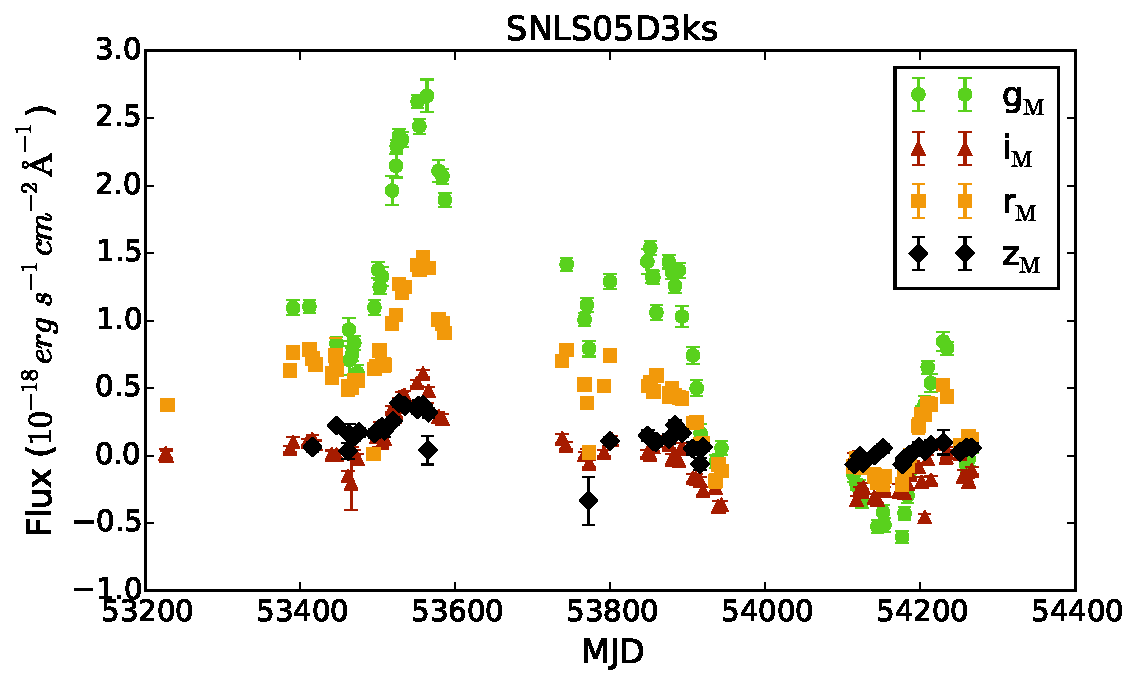
\includegraphics[width=\textwidth]{Figures/Chapter3/SNLS05D3ks}
\caption{The $g_M$, $r_M$, $i_M$, $z_M$ multi-season light curve of SNLS-05D3ks. This transient is found within the SLSN parameter space (\fref{fig:SLAPparam}), but does not pass visual inspection as it shows clear signs of multiple maxima.}
\label{fig:05D3ks}
\end{figure}

\subsection{SNLS-07D3bs}
\label{sec:07D3bs}
SNLS-07D3bs is identified as a SLSN candidate between $0.6<z<1.2$ based on its host galaxy photometric redshift estimate. The best-fit magnetar model for the object is obtained at z = 1.0. While SNLS-07D3bs was never classified or recognised as an object of interest during the life of SNLS, it has been spectroscopically observed on the 17$^{\mathrm{th}}$ April 2007 using the Keck/LRIS instrument. This data was never published officially as no spectral classification was obtained at that time. The data was however presented in a PhD thesis by \citet{Fakhouri2013}.

At the time the observations of SNLS-07D3bs were made, the SLSN class was not yet known and no SLSN spectral templates were available for comparison with the data. It is also because of this that the SLSN that have been previously identified in SLSN by \citet{Howell2013} have not been originally identified as objects of interest until several years after their initial detection. Using the \textsc{superfit} spectrum identification tool \citep{Howell2005}, the spectrum of SNLS-07D3bs was re-analysed by fitting all available SN templates at a broad range of redshifts exceeding our photometric estimate. The data are noisy with a signal-to-noise $\sim$ 7 as observing conditions were quite poor. Despite this, I find the best spectral match to be to the SLSN iPTF13ajg at $z=0.757$ as can be seen in \fref{fig:07D3bsSpec}. While this is clearly an uncertain spectral classification, there is no evidence from the spectrum that the object is not a SLSN, particularly as the best match is an event of that type. The magnetar model also provides a good fit at that redshift as seen in  \tref{tab:07d3bsParams}. The host galaxy, located at RA=14h~21m~50.466s, Dec=+53$^{\circ}$~10'~28.58'', is detected in the SNLS deep stack images \citep{Ilbert2006}, but is very faint, with AB magnitudes of ($u_M$, $g_M$, $r_M$, $i_M$, $z_M$) = ($26.61\pm0.49$, $26.13\pm0.16$, $25.67\pm0.13$, $25.18\pm0.11$, $25.19\pm0.37$). Combining the spectral and magnetar model fitting, as well as a faint host galaxy, matching the properties expected of most SLSNe, provided us with sufficient evidence to consider SNLS-07D3bs to be the third SLSN detected by the real-time pipeline of SNLS.

\begin{figure}
\centering
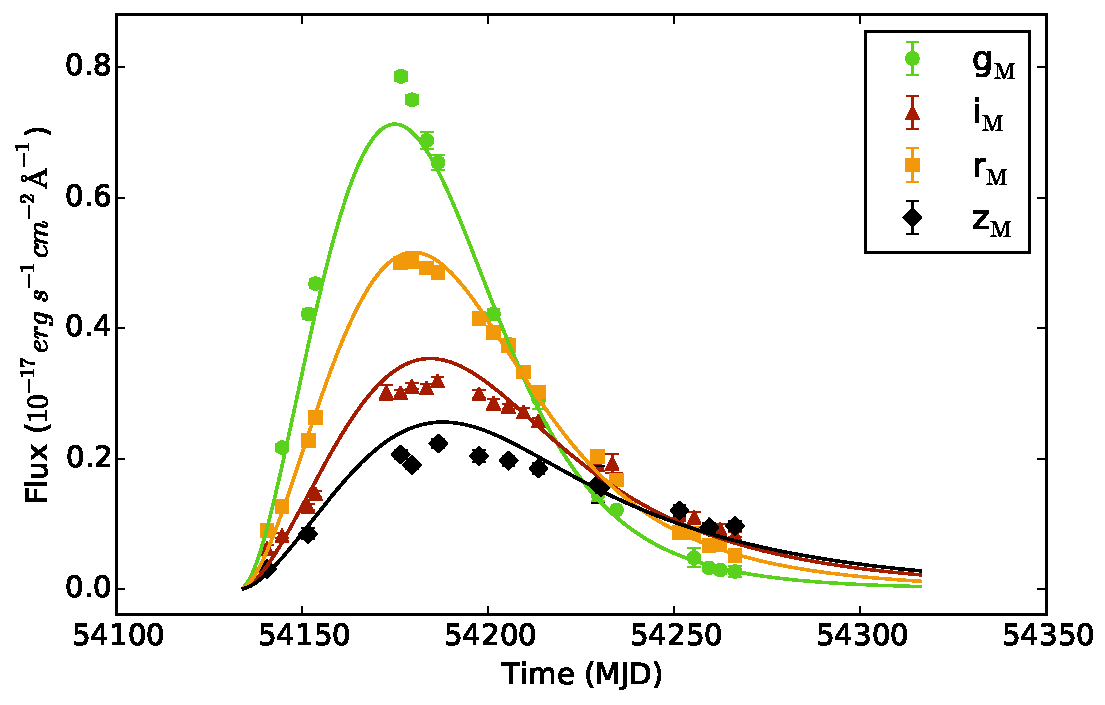
\includegraphics[width=\textwidth]{Figures/Chapter3/07D3bs}
\caption{The $g_M$, $r_M$, $i_M$, $z_M$ light curve of SNLS-07D3bs overplotted with the best-fit magnetar model at $z=0.757$. The candidate shows a good agreement with the model.}
\label{fig:07D3bsLC}
\end{figure}

\begin{figure}
\centering
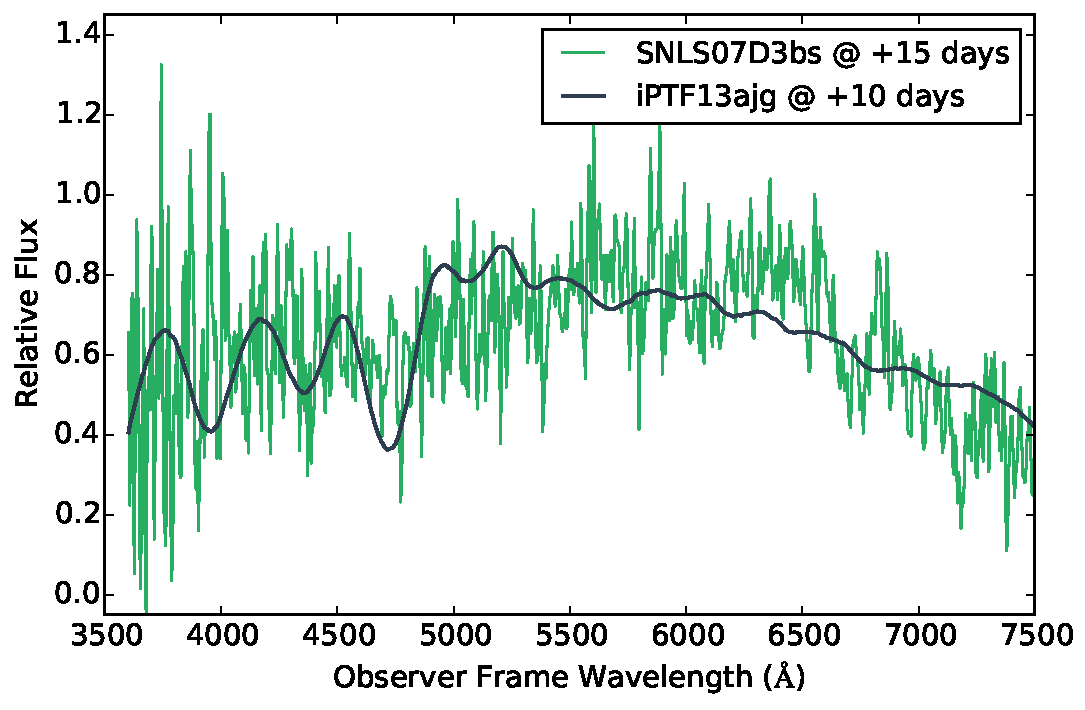
\includegraphics[width=\textwidth]{Figures/Chapter3/07D3bsSpec}
\caption{The spectrum of SNLS-07D3bs from Keck/LRIS, taken 15 rest-frame days after maximum light. The signal-to-noise of the spectrum is low preventing a definitive classification; however, the spectrum is consistent with a SLSN at around $z=0.76$. Weak galaxy emission lines are consistent with $z=0.757$.}
\label{fig:07D3bsSpec}
\end{figure}

\begin{table}
\begin{center}
\caption{Magnetar model parameters for the new SNLS SLSN candidate: SNLS-07D3bs.}
\label{tab:07d3bsParams}
\begin{tabular}{|l|r|r|r|r|r|r|r|r|r|r|}
\hline
  \multicolumn{1}{|c|}{Name} &
  \multicolumn{1}{c|}{$M_u$} &
  \multicolumn{1}{c|}{$t_\mathrm{rise}$} &
  \multicolumn{1}{c|}{$\tau_\mathrm{m}$} &
  \multicolumn{1}{c|}{$B_{14}$} &
  \multicolumn{1}{c|}{$P_{\mathrm{ms}}$} &
  \multicolumn{1}{c|}{$t_\mathrm{expl}$} &
  \multicolumn{1}{c|}{$E(B-V)$} &
  \multicolumn{1}{c|}{$\chi^2_{\nu}$} &
  \multicolumn{1}{c|}{Template} \\ & &
  \multicolumn{1}{c|}{(days)} &
  \multicolumn{1}{c|}{(days)} &
  \multicolumn{1}{c|}{($\times10^{14}$ G)} &
  \multicolumn{1}{c|}{(ms)} &
  \multicolumn{1}{c|}{(MJD)} & \\
\hline
SNLS-07D3bs & -20.9 &  27.2 & 23.7 & 2.28 & 3.81 & 54132.5 & 0.05 & 1.96 & iPTF13ajg\\
\hline
\end{tabular}
\end{center}
\end{table}

\section{The rate of superluminous supernovae}
\label{sec:MC}
In the previous sections I have outlined our approach to selecting a suitable definition of SLSNe before applying it to a sample of transient detected by the SNLS. This resulted in identifying a sample of three SLSNe including two previously known objects and a new, previously unclassified example; SNLS-07D3bs. In this section I describe the method used to calculate the volumetric rate of SLSNe, $\rho_{\mathrm{slsn}}$, implied by these detections. First, I describe the method used for this calculation and the reasoning behind our use of a Monte-Carlo simulation over a purely statistical approach. I then discuss the reasoning behind our choice of the search volume before presenting the rate calculation and the result.

\subsection{Defining a rate}
\label{sec:method}
$\rho_{\mathrm{slsn}}$ can be defined as a sum over the number of SLSNe, $N$, found in a given comoving search volume, $V$, over a search duration, $t$, weighted by the inverse of the detection efficiency, $\epsilon_{i}$, of detecting each event. This can be summerised using \eref{eq:rate}:

\begin{equation}
\label{eq:rate}
\rho_{\mathrm{slsn}} = \frac{1}{V}\sum^{N}_{i}\frac{(1+z_i)}{\epsilon_{i}t_{i}}.
\end{equation}

The factor $(1+z_i)$ corrects for time dilation. The detection efficiency $\epsilon_i$ is a statistic describing how each SLSN should be weighted relative to the whole population. In other words, $1-\epsilon_i$ gives the fraction of similar SLSNe that exploded during the search period but were missed by the survey due to, for example, search inefficiencies. The detection efficiency is a vital and simultaniously the most difficult part of the computation.

\subsection{Detection efficiency}
The full treatment of a detection efficiency for any survey is a very complex problem with many aspects of the survey to be considered including the cadance, image quality, limiting magnitude amongst other. \citet{Frohmaier2017} shows a recent examples of such comprehensive study performed with the aim of calculating the local volumetric rate of SNIa in PTF. Our SLSN detection efficiencies is based on a similar analysis by \citet{Perrett2010}, who carried out a study of the detection efficiencies and selection biases of SNIa in SNLS, and subsequently calculated a rate of those events in \cite{Perrett2012}. In this study, several million fake SNIa were placed in the SNLS science images, with the correct temporal evolution, and passed through the SNLS real-time detection pipeline. The recovery efficiencies of these SNe Ia could then be estimated. Although these results were produced using a particular model of a particular supernova type, at a more basic level they also provide the recovery efficiencies of point sources in the SNLS data as a function of magnitude in every $i_M$-band image that SNLS took, and it is these more basic data that we use in this study. [MAKE A PLOT SHOWING WHAT THAT LOOKS LIKE FOR A RANDOM OBSERVING EPOCH]

\subsection{Method}
In this work, I reverse the common approach to supernova rate calculations, such as the ones used by \citet{Perrett2012} and \citep{Frohmaier2017}. Instead of calculating the rate of SLSNe starting with the number of detected objects, I calculate the probability that a given initial value of $\rho_{\mathrm{slsn}}$ leads to an eventual detection of three SLSNe in the survey. This method is capable of producing a non-Gaussian uncertainty estimate as a by-product of the calculation as the result is presented in form of a probability distribution (\fref{fig:rateFlat3}). The uncertainties can be simply quoted as the 1$\sigma$ confidence region of this distribution.

To simulate the SLSN population in SNLS I use a Monte Carlo approach. I 'explode' fake SLSNe randomly within the SNLS search period and search volume, and create artificial SLSN light curves on each epoch corresponsing to the SNLS observations, including the effect of $1+z$ time dilation. As a result it is possible to measure the $i_M$ apparent magnitude on each epoch, which is then compared to the point-source recovery statistics on that epoch to give the probability of detection. I combine all of these individual probabilities to give us an overall detection probability per object.

\subsection{Search volumes}
\label{sec:search-volumes}
The effective SNLS search areas for each field, from which the search volumes can be calculated, was found accurately in \citet{Perrett2012} giving an effective total search area of 3.56\,deg$^2$. The volume is calculated by considering the redshift range to which our search was sensitive. The four observing fields cannot all be considered as identical there are small variation in the detection efficiency amongst the fields. The observing season in the D3 field was longer in comparison to the other fields while D1 and D2 had on average, marginally deeper exposures.

At the low-redshift end, the search volume is set by the redshift at which a SLSN would become saturated in the SNLS data. At the high-redshift end, the volume is set by the redshift at which we are no longer able to recover a SLSN event, i.e. a SLSN would fall below the detection limit of the survey. \fref{fig:zrange} illustrates the redshift range to which the search for SLSNe is sensitive to in SNLS, showing the recovery efficiency as a function of redshift for the three events identified in \sref{sec:SLSNCands}. For events at z $<$ 0.2, the efficiency drops rapidly due to saturation effects setting z = 0.2 as the lower redshift limit. At the upper redshift limit, I choose z = 1.6. Although some events similar to SNLS-06D4eu are detectable at z > 2, the fainter events like SNLS-07D3ds would become undetectable in some of the SNLS search fields at z $<$ 1.6.

\begin{figure}
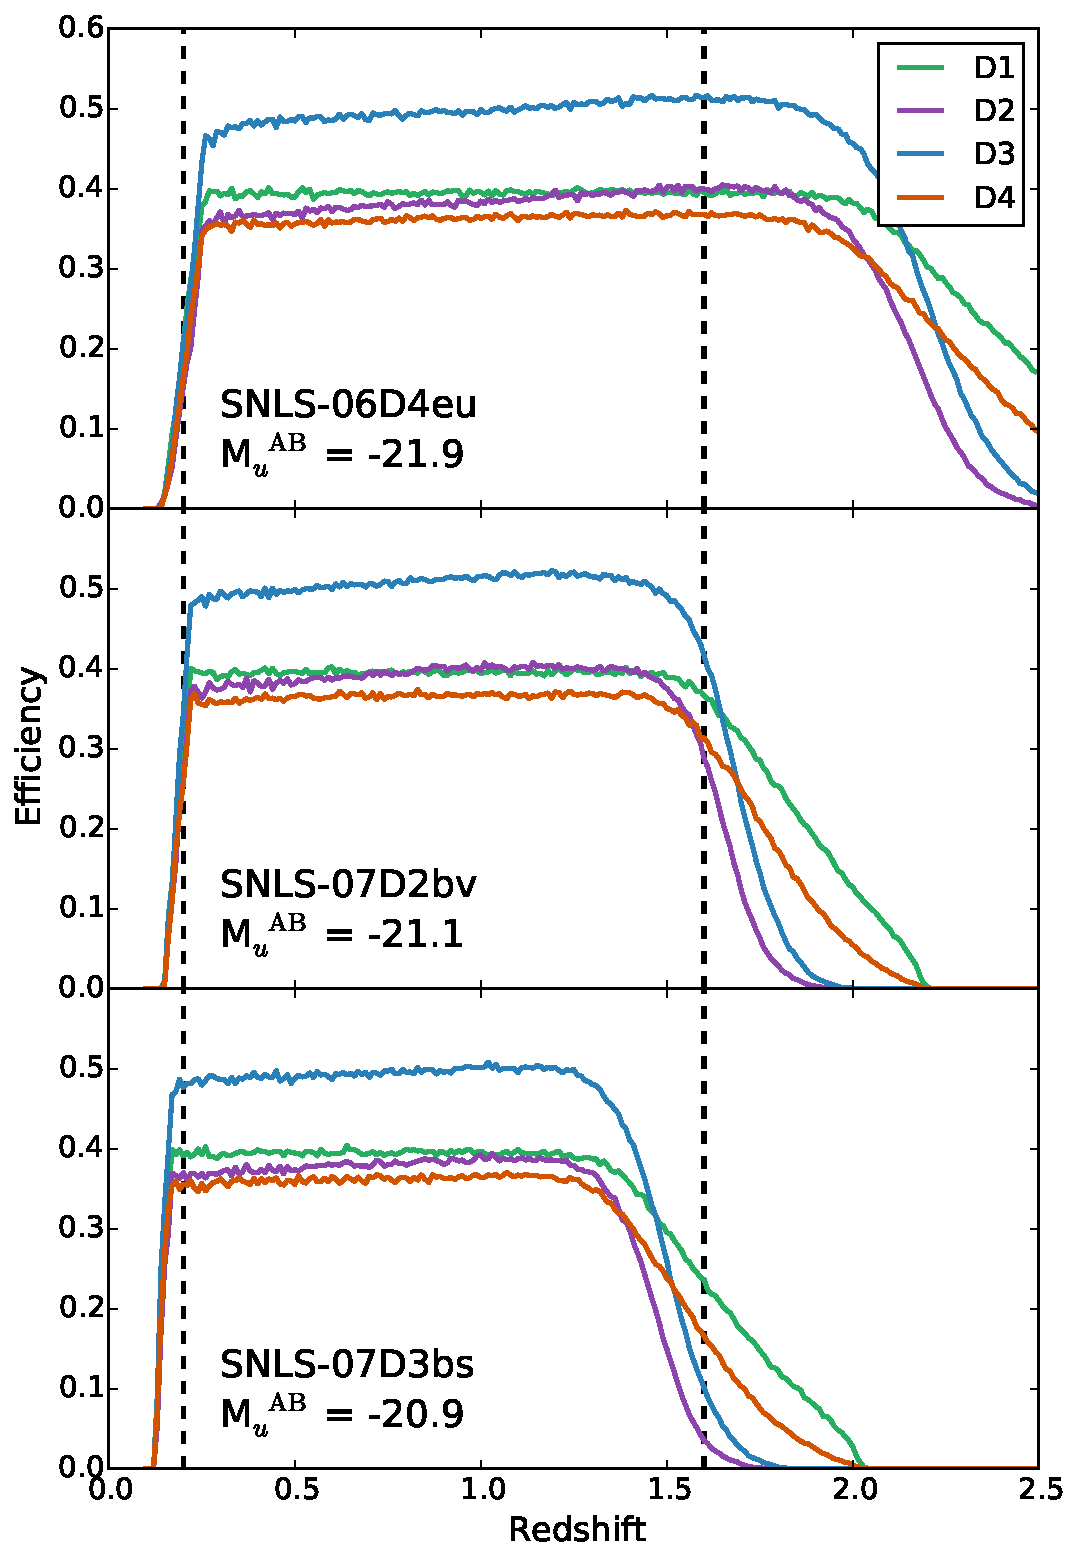
\includegraphics[width=\textwidth]{Figures/Chapter3/Efficiency}
\caption{The redshift range to which our SLSN search is sensitive to, as a function of the four SNLS search fields. The figure shows the recovery efficiency of three different SLSNe as a function of redshift, with each line corresponding to a different search field. The efficiency includes the same data quality cuts as used in the training sample in \sref{sec:Definition} and the SNLS candidate selection in \sref{sec:SLSNCands}. The vertical dashed lines at z = 0.2 and z = 1.6 illustrate the final redshift range used in our Monte Carlo rate calculations.}
\label{fig:zrange}
\end{figure}

\subsection{Monte Carlo simulation}
\label{sec:rate-calculation}
I begin each Monte Carlo simulation with an input $\rho_{\mathrm{slsn}}$ value. From this I calculate the number of SLSNe that would have occurred within the SNLS search area over the redshift range to which we are sensitive ($0.2<\mathrm{z}<1.6$) in bins of $\Delta$z = 0.01. I assume that this rate does not evolve within the redshift range considered in our simulation.Hhowever, this assertion is later tested \sref{sec:SFRRate}. The artificial SLSNe are then assigned a random spatial position (and consequent Milky Way extinction), redshift, host galaxy extinction and physical parameters drawn from the magnetar model parameter space derived from our training sample (\fref{fig:SLAPparam}). A random explosion epoch during the SNLS search period is assigned to each event. From this the synthetic photometry was calculated on every epoch corresponding to a SNLS observation.

Using the point-source detection efficiencies of \cite{Perrett2010}, I calculate the probability of detecting each SLSN on every epoch of $i_M$ data, and combine the probabilities to give the total probability of discovering each object. In order to be considered detected, I enforce that each artificial SLSN must pass the same data quality cuts as both our training sample in \sref{sec:Definition} and our real sample of SNLS candidates in \sref{sec:SLSNCands}. I repeate the entire simulation 100,000 times over an input $\rho_{\mathrm{slsn}}$ range of $5 \leq \rho_{\mathrm{slsn}} \leq 500$\,SNe\,Yr$^{-1}$\,Gpc$^{-3}$.

\fref{fig:rateFlat3} shows the probability of three SLSN events being detected in our simulations as a function of the input rate. A log-normal distribution is fitted to the simulation results and used to smoothly determine the peak of the distribution as well as the 1$\sigma$ confidence regions. From this, we find the rate of SLSNe at z = 1.13, which is the volume-weighted centre of the 0.2 $<$ z $<$ 1.6 range, to be $\rho_{\mathrm{slsn}} = 91^{+76}_{-36}$\,SNe\,Yr$^{-1}$\,Gpc$^{-3}$.

\begin{figure}
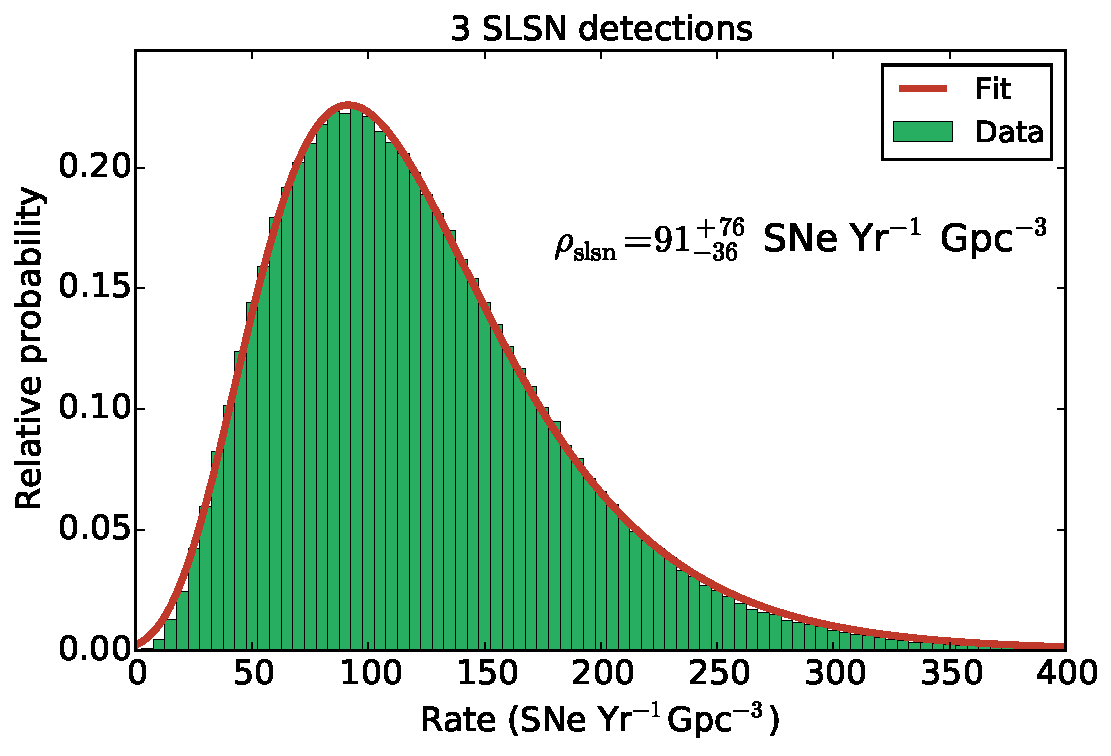
\includegraphics[width=\textwidth]{Figures/Chapter3/rateFlat3}
\caption{The probability distribution of the volumetric rate of SLSNe for the three SLSN candidates over the duration of SNLS at 0.2 $<$ z $<$ 1.6, as determined by our 100,000 Monte Carlo simulations. A log-normal distribution is fit to the data (red line) to estimate the peak of the probability distribution and the uncertainties, quoted as the 68\% confidence region.}
\label{fig:rateFlat3}
\end{figure}

\subsection{Rate assuming a SFR distribution of SLSN}
\label{sec:SFRRate}
As SLSN are a likely consequence of a collapse of a giant star with an intrinsicly fast stellar evolution, it is expected that the rate of SLSNe should follow closely to that of their birth, i.e the cosmic star formation rate (SFR). An expected consequence of this would be that a larger proportion of SLSNe are found at high redshift compared with a non-evolving population. I investigate the consequence of this effect on our final rate by repeating the Monte Carlo simulation, instead drawing the SLSNe from a redshift distribution that follows the cosmic star-formation history as taken from \citet{2006ApJ...651..142H} and described in more details in \sref{sec:ConclusionsSFR}. For the value pivoted at z=1.13, as in the case of the flat distribution, I find $\rho_{\mathrm{slsn}} = 98^{+82}_{-39}$\,SNe\,Yr$^{-1}$\,Gpc$^{-3}$. This is very close to the original result and, considering the uncertainities, a negligible difference. Thus our final rate, averaged over the redshift range we have considered, is not sensitive to the assumed rate evolution in our simulation. One possible explanation of this is that the relative uniformity of our detection efficiency as a function of redshift within our search volume has negated the effects of the redshift evolution (\fref{fig:zrange}).

\section{Discussion}
Having calculated the rate of SLSNe at an intermediate redshift, it is now interesting to compare the value to other measurements and study its evolution as a function of redshift.

\subsection{Rate Evolution with Redshift}
\label{sec:Discussion}
\begin{figure}
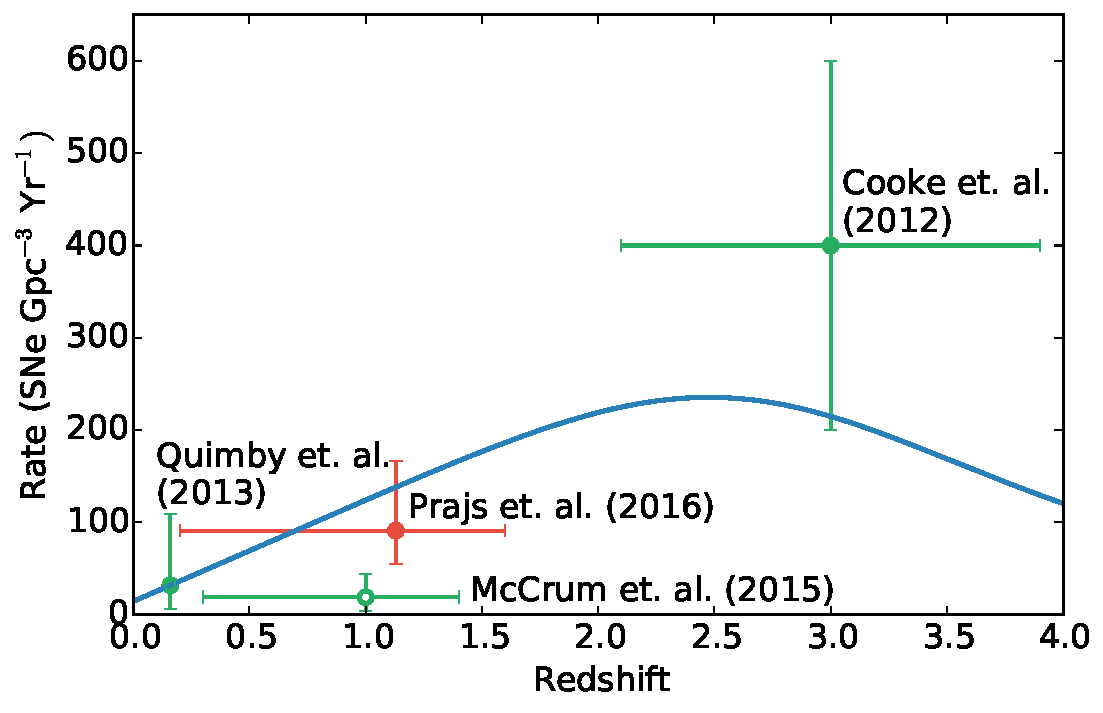
\includegraphics[width=\textwidth]{Figures/Chapter3/rate}
\caption{The evolution of the volumetric SLSN rate as a function of redshift. I compare my measurement to those by \citet{Cookie2013}, \citet{Quimby2014} and \citet{McCrum2015} for comparison. The \citet{McCrum2015} result is marked by an open circle to highlight that it may not be directly comparable with the other measurements as it is derived by a comparison to the rate of core collapse supernovae and is not a direct measurement. The observed evolution is consistent with that of the SFH over the same redshift range; I over-plot in blue the parametrisation of the cosmic SFH of \citet{2006ApJ...651..142H}, normalised to the low-redshift SLSN-I rate obtained by \citet{Quimby2014}.}
\label{fig:rate}
\end{figure}

\fref{fig:rate} shows the SLSN rate calculated in this chapter compared with the values published by \citet{Cookie2013}, \citet{Quimby2014} and \citet{McCrum2015}. The volumetric rate increases as a function of redshift with the extent of this observed evolution is consistent with the evolution in the cosmic star-formation history observed over the same redshift range \citep{2006ApJ...651..142H}. This is, perhaps, an unsurprising result, as SLSNe are thought to originate from the death of very massive and hence short-lived stars. However, it is important to note here, that we are not able to discriminate between the evolution that follows the star formation history, and one with the same evolution up to $z=1.5$ but followed by a peak at a much higher redshift, as the $z>1.5$ measurement is quite uncertain.

In fact, a higher-redshift peak of the rate may be expected as SLSNe are almost exclusively explode in galaxies that are low-mass, compact dwarfs \citep{2011ApJ...727...15N,2015ApJ...804...90L}, and that are metal-poor and strongly star-forming \citep{2013ApJ...771...97L,2013ApJ...763L..28C,2015MNRAS.449..917L}. One popular interpretation of this is that the low metallicity must play a role in the formation of SLSNe, which is consistent with the low metal content inferred from their UV spectra \citep{Mazzalli2016}. This scenario would also predict a volumetric rate evolution that follows both the cosmic SFH and cosmic chemical enrichment. The possibility of testing the originins of SLSNe and the role of metal enrichment to their formation gives one of the strongest motivations behind the future studies of their rates at $z>2$.

\subsubsection{Comparison to the rate of CCSN}
Comparing the rate of SLSNe to that of CCSN is yet another particularly interesting test which can inform us about their origin. Using SLSNe discovered by the Pan-STARRS medium deep survey over $0.3 \leq z \leq 1.4$, \citet{McCrum2015} measure the relative rate of SLSNe to be between $3^{+3}_{-2}\times10^{-5}$ and $8^{+2}_{-1}\times10^{-5}$ that of the core-collapse supernova rate, $\rho_{\mathrm{cc}}$. We use the SNLS $\rho_{\mathrm{cc}}$ measurement at $z\sim0.3$ of $1.42\pm0.6\times10^{-4}$ \,SNe\,Gpc $^{-3}$ \,yr $^{-1}$ \citep{2009A&A...499..653B}, and extrapolate it to $z=1.13$, assuming it tracks the cosmic SFH, increasing the rate by a factor of 2.62. Our own absolute SLSN rate can then be expressed as rate relative to that of core collapse SNe, which we find to be 2.2$^{+1.8}_{-0.9}\times10^{-4}$ of the $\rho_{\mathrm{cc}}$. This is higher than, but still consistent with, the relative rate of \citet{2015MNRAS.448.1206M}. [WRITE ABOUT THE MEANING]

\subsection{Host Galaxies of SNLS SLSNe}
The host galaxies of SLSNe play a key factor in their study. Beside playing a factor in determining their origings they also provide an observable that could act as a further confirmation for a photometrically selected object. \fref{fig:hosts} shows the distribution of SLSN host-galaxy stellar masses as measured by \cite{Lunnan2014}. We use the \textsc{zpeg} photometric redshift package \citep{2002A&amp;A...386..446L} with the SNLS multi-waveband $g_M$,$r_M$,$i_M$,$z_M$ host galaxy photometry to estimate the stellar mass for SNLS-07D3bs. We are not able to derive host galaxy stellar masses for SNLS-06D4eu and SNLS-07D2bv using the SNLS deep stacks due to the galaxies faintness and the lack of infrared (which correspond to the rest-frame optical) data. We instead use values obtained by \citet{Leloudas2015a} and \citet{Schulze2017}. The host stellar masses for all three of our candidates agree with the published SLSN-I host stellar mass distribution as showed in \fref{fig:hosts}.

\begin{figure}
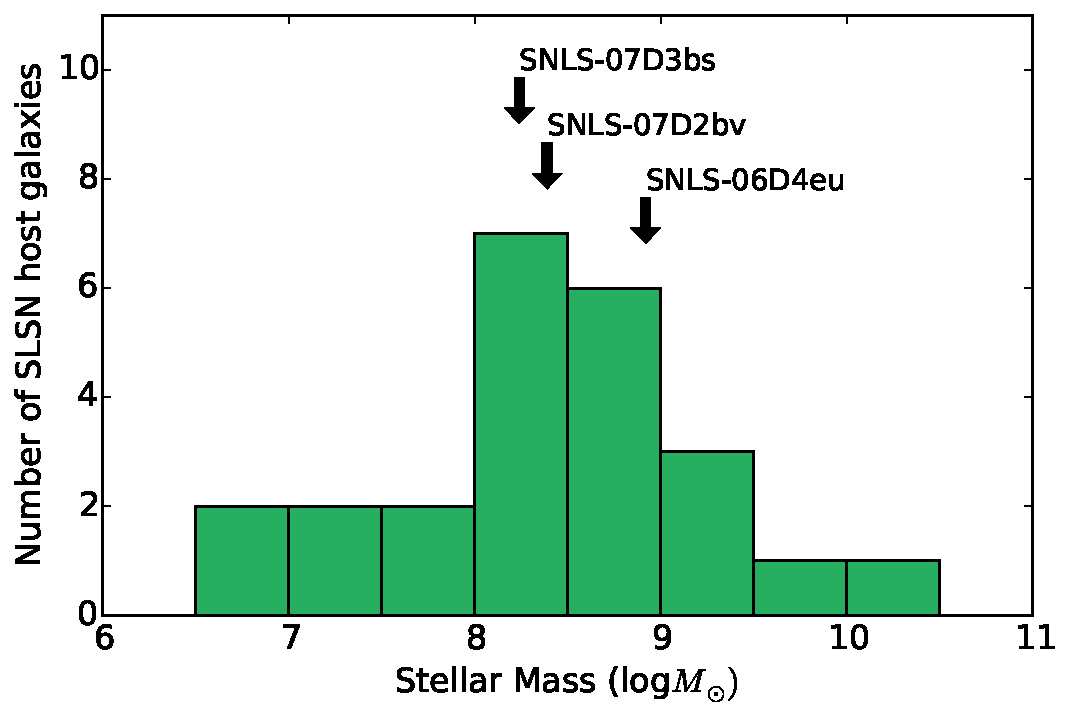
\includegraphics[width=\textwidth]{Figures/Chapter3/Galaxy}
\caption{The stellar mass distribution of SLSN host galaxies plotted using the data from \citet{Lunnan2014}, showing the consistency of SNLS07D3bs with the rest of the population. The lack of detections for the hosts of the high redshift candidates is consistent with being associated with low mass galaxies, found below the detection limit of SNLS at their redshifts.}
\label{fig:hosts}
\end{figure}
 % Experimental Setup

%\chapter{Techniques}
\label{Chapter4}
\lhead{Chapter 4. \emph{Codes}}

Throughout this thesis my goals were to identify SLSNe in a number of surveys. I have approached this problem using a number of tools and techniques, each playing an important role in achieving this goal. The aim of this chapter is to provide and overview of the methods used in this work as well as their evolution over time. In the early parts of this thesis, I used an approached based on modelling of SLSNe using the popular spin-down of a magnetar model \sref{sec:SLAP}. I begin by describing the model and the improvements I have introduces in order to better model the UV region of the SLSN SED. I also describe the fitting routines used in the modelling of SLSNe as well as throughtout the entire thesis. Although, this technique was successful in identifying a new SLSN in the SNLS, it was not able to fully capture the diversity of the SLSN sample that was emerging in the DES spectroscopic dataset. As a solution to this problem, I followed a popular route of applying the state-of-the-art artifficial inteligence (AI) technqiues to automate the classification process using a machine learning approach. The second part of this chapter describes the preparatory work undertaken to build the tools and the training sample required for such study in \cref{Chapter5}.

The use of ML moved the focus of this work away from understanding the parameter space of the SLSNe model, or the choice of cuts needed to define them. Instead I have focused on simulating DES and its tranients. This includes SNIa, both hydrogen poor and rich CCSNe, SLSNe, AGNs as well as random noise spikes which are the main source of contamination in the data. The models of SNIa are mature and ready to be deployed in this work thanks to being used as cosmological probes for over two decades. Simulations of CCSNe, however, have not sparked an equal amount of enthusiasm amonst the SN community until recently, hence became a one of the key subjects of this thesis. CCSN are usually faster and fainter than SNIa resulting is a significantly smaller sample of well observed objects. The number of objects with a high quality spectroscopic follow-up are also much lower compare to SNIa. In recent years, the interest in modelling these objects has increased dramatically with large projects, such as LSST, requiring samples of fake transients in order to inform the design of their observing strategies. In this chapter, I describe our approach to creating a new spectroscopic set of CCSN templates as well as simulating them in a number of surveys. This project was build to provide a sample of stripped-envelope CCSNe as part of the LSST photometric lightcurves classification challenge. However, later I have applied it to DES in order to produce both a samples of hydrogen rich as well as poor CCSNe.

The last, but perhaps the most important, technique descrined in this chapter is Gaussian Processing (GP). DES, similarly to other transient surveys, was not observed on regular cadance. However, most machine learning techniques require evenly samples data. I used Gaussian Processes as a method for interpolating the light curves independantly of any model which could be used to simualate the objects. GPs are based only on the uncertainties associated with the data and produce a confidence regions for the underlying light curves. This is key in solving the overfitting problem when working with artificial training sample within Machine Learning.

This chapter is divided in the following way; I begin by describing the methods behind the modelling of SLSNe using the magnetar model as well some some basic extensions in conjunction with SED templates. Following this, I discuss the search for SLSNe as well as their pre-peak `bumps' and other rapidly evolving transients in DES. Next, I describe the method of Gaussian Processing light curves as a model-independant approach to interpolating our data. Finally, I describe the techniques behind the modelling and simulating of CCSN in the context of DES.

\section{Modeling SLSN Light Curves} \label{sec:SLAP}
Throughout this thesis the modelling of SLSNe light curves plays a pivotal role. The measurement of the rate of SLSNe presented in \cref{Chapter3} as well as the search for SLSNe in DES described in \cref{Chapter5,Chapter6} uses a definition of SLSNe based on the spin-down of the magnetar model. The choice of the magnetar model as our main tool came after a simpler model, describing SLSNe using and linearly expanding and cooling photosphere, was tested but eventually rejected in favour of the magnetar model. I introduce this basic model, including its drawbacks, before I describe the magnetar model along with the improvements it brings to the modelling of SLSNe.

When modelling light curves of SLSNe there are two independant, but equally important, areas that contribute to the accuracy of the model: the spectral energy distribution (SED) of the SN, and its evolution with time. The need to model the SED of a SN could be avoided if we used an approach which purely relied on the bolometric lightcurves as opposed to multi-band observations. From the software implementation point-of-view these models are easier to use, and are common in the literature \citep{Inserra2013,Papadopuplus2014,Nicholl14}. However, they do not consider the colour, along with its evolution, of a SN which provides a very powerful tool for further constraints the properties of the SNe. It has been previously shown \citep{2011ApJ...743..114C,2013ApJ...779...98H,2015MNRAS.449.1215P,2014ApJ...797...24V} that the SLSN SED can be accurately approximated, in the visible spectrum, by a slowly evolving (nearly) perfect blackbody with an addition of their characteristic broad lines of O\,II. However, this approximation breaks down in the near UV due to the prominant broad absorption features which can be attributed to Mg\,II, Fe\,III, C\,II, Co\,III, Si\,III and Ti\,III \citep[see][for line identifications]{Mazalli2016}.

\subsection{Improving the blackbody approximation}
In order to improve the reliability of SLSN SED modelling, I propose a method of improving the blackbody approximation by superimposing absorption template onto the simple blackbody SED. In order to derive these template, I use a method similar to tht of  \citet{2014ApJ...797...24V} where I fit the Planck function to several featureless, 50$\AA$ wide regions of the spectrum in order to measure the underlined blackbody continuum in the SED, as shown in figure \ref{fig:specTemplate}. The resulting fits show that the absorption relative to the blackbody is low in the regions of $\lambda>3000\AA$, and increases drastically in the bluer regions of the spectrum.

The time evolution of the spectra appears to be weak in comparison to other SNe, making it possible to approximate the SED at any epoch using the Planck function, where the temperature evolves with time, and a single absorption template is used. The absorption is calculated as a ratio of the observed flux to the continuum blackbody fit. The number of SLSNe with good UV coverage remains small, with only the spectra of iPTF13ajg \citep{2014ApJ...797...24V}, SCP06F6 \citep{2009ApJ...690.1358B} and SNLS-06D4eu \citep{2013ApJ...779...98H} providing sufficient data until the discovery of Gaia[CITE AND INSERT NUMBERS]. Do due to the observer-frame coverage of their respective spectra, our spectral templates cover a rest-frame wavelength range of 1620--3320\,\AA\ (SNLS-06D4eu), 1800--3800\,\AA\ (SCP06F6) and 1800--5250\,\AA\ (iPTF13ajg). [PERHAPS REMOVE THIS TO MAKE IT LESS HARD ON MYSELF]
\begin{figure}
\centering
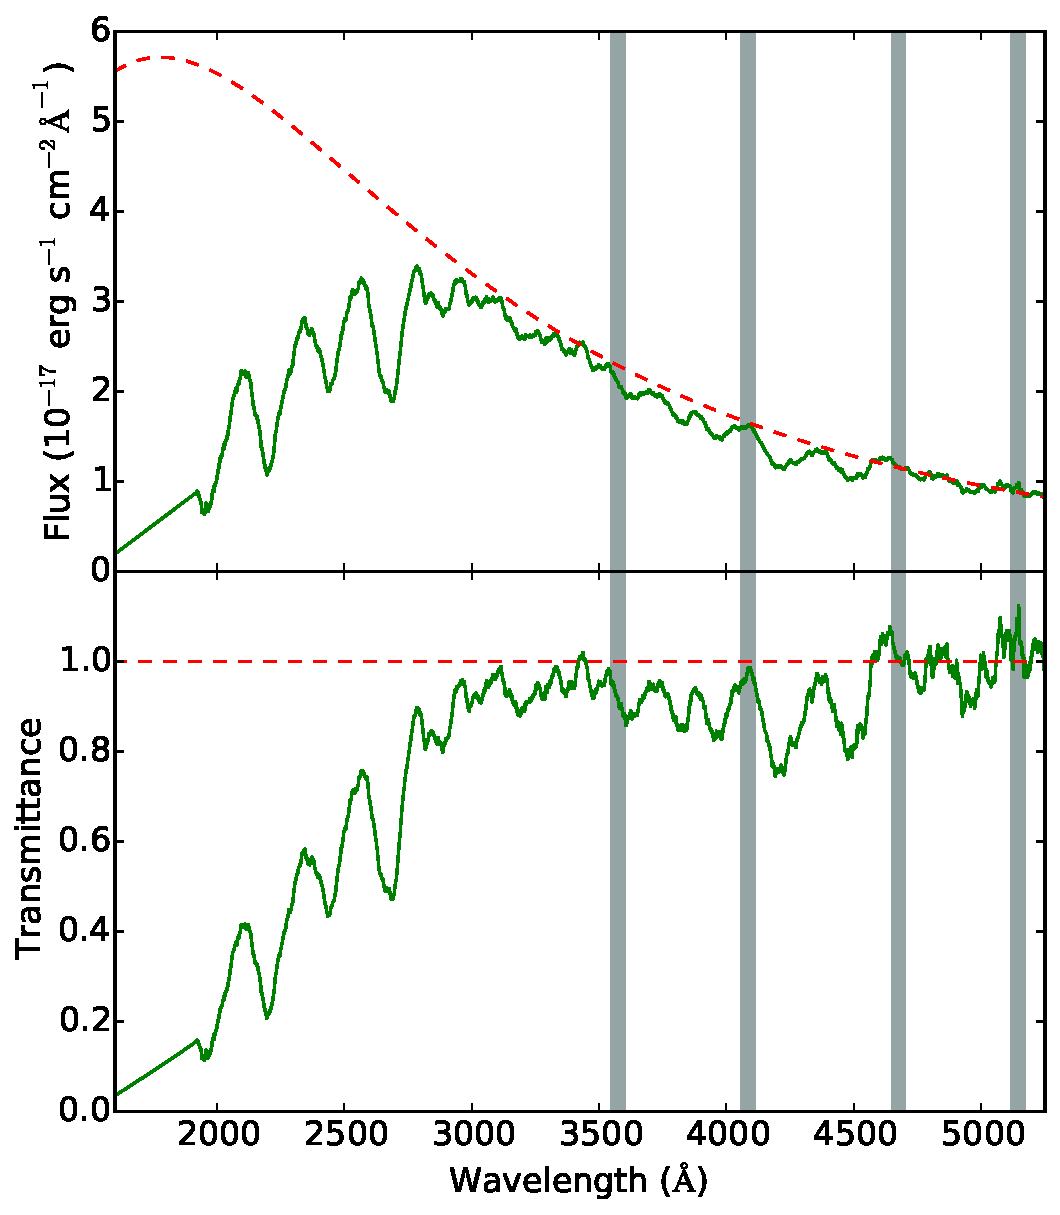
\includegraphics[width=\textwidth]{Figures/Chapter4/specTemplate}
\caption{iPTF13ajg is fitted with the Planck function. The spectrum of iPTF13ajg (green) can shows a good agreement with the blackbody (red) at $\lambda>3000\AA$. At lower wavelengths a strong deviation from the model is observed, highlighting the need for a correction to the model. The ratio between the observed spectrum and the continuum give a measure of the absorption strength as a function of wavelength and can be used in modelling the SLSN SED.}
\label{fig:specTemplate}
\end{figure}

\subsection{Modelling the SED evolution}
The ability to describe the SEDs of SLSNe as blackbodies greatly simplies the
modelling of its evoution. A model is only required to provide the thermal and radial evolution of the photoshere, therefore removing the need for complex modelling such as radiative transfer or hydrodynamic simulations.

\subsubsection{Fireball model}
Perhaps the simplest approach to modelling the SED evolution is to assume that the SN, with an initial radius R$_{0}$ and initial temperature T$_{0}$ expands at a constant rate while cooling down also at a current rate as seen in \eref{eq:Howell}
\begin{align}
\label{eq:Howell}
R(t) &= R_0 + \dot{R}t &&\\
T(t) &= T_0 - \dot{T}t &&
\end{align}
\noindent While this model is not physical motivated, \citet{Howell2013} showed that it provides a good, first-order approximation to the light-curves of SLSNe. Due to its simplicity, the model appeared as an attractive prospect for the modelling of SLSN SEDs. However, our testing showed that while it produces a good fit to a SLSN around the maximum light (<+30days) it is not able to capture the slow evolution in the tale of the light curve as seen in \fref{fig:BB_Mag} making in infavarable in comparison with the more complex magnetar model.

\begin{figure}
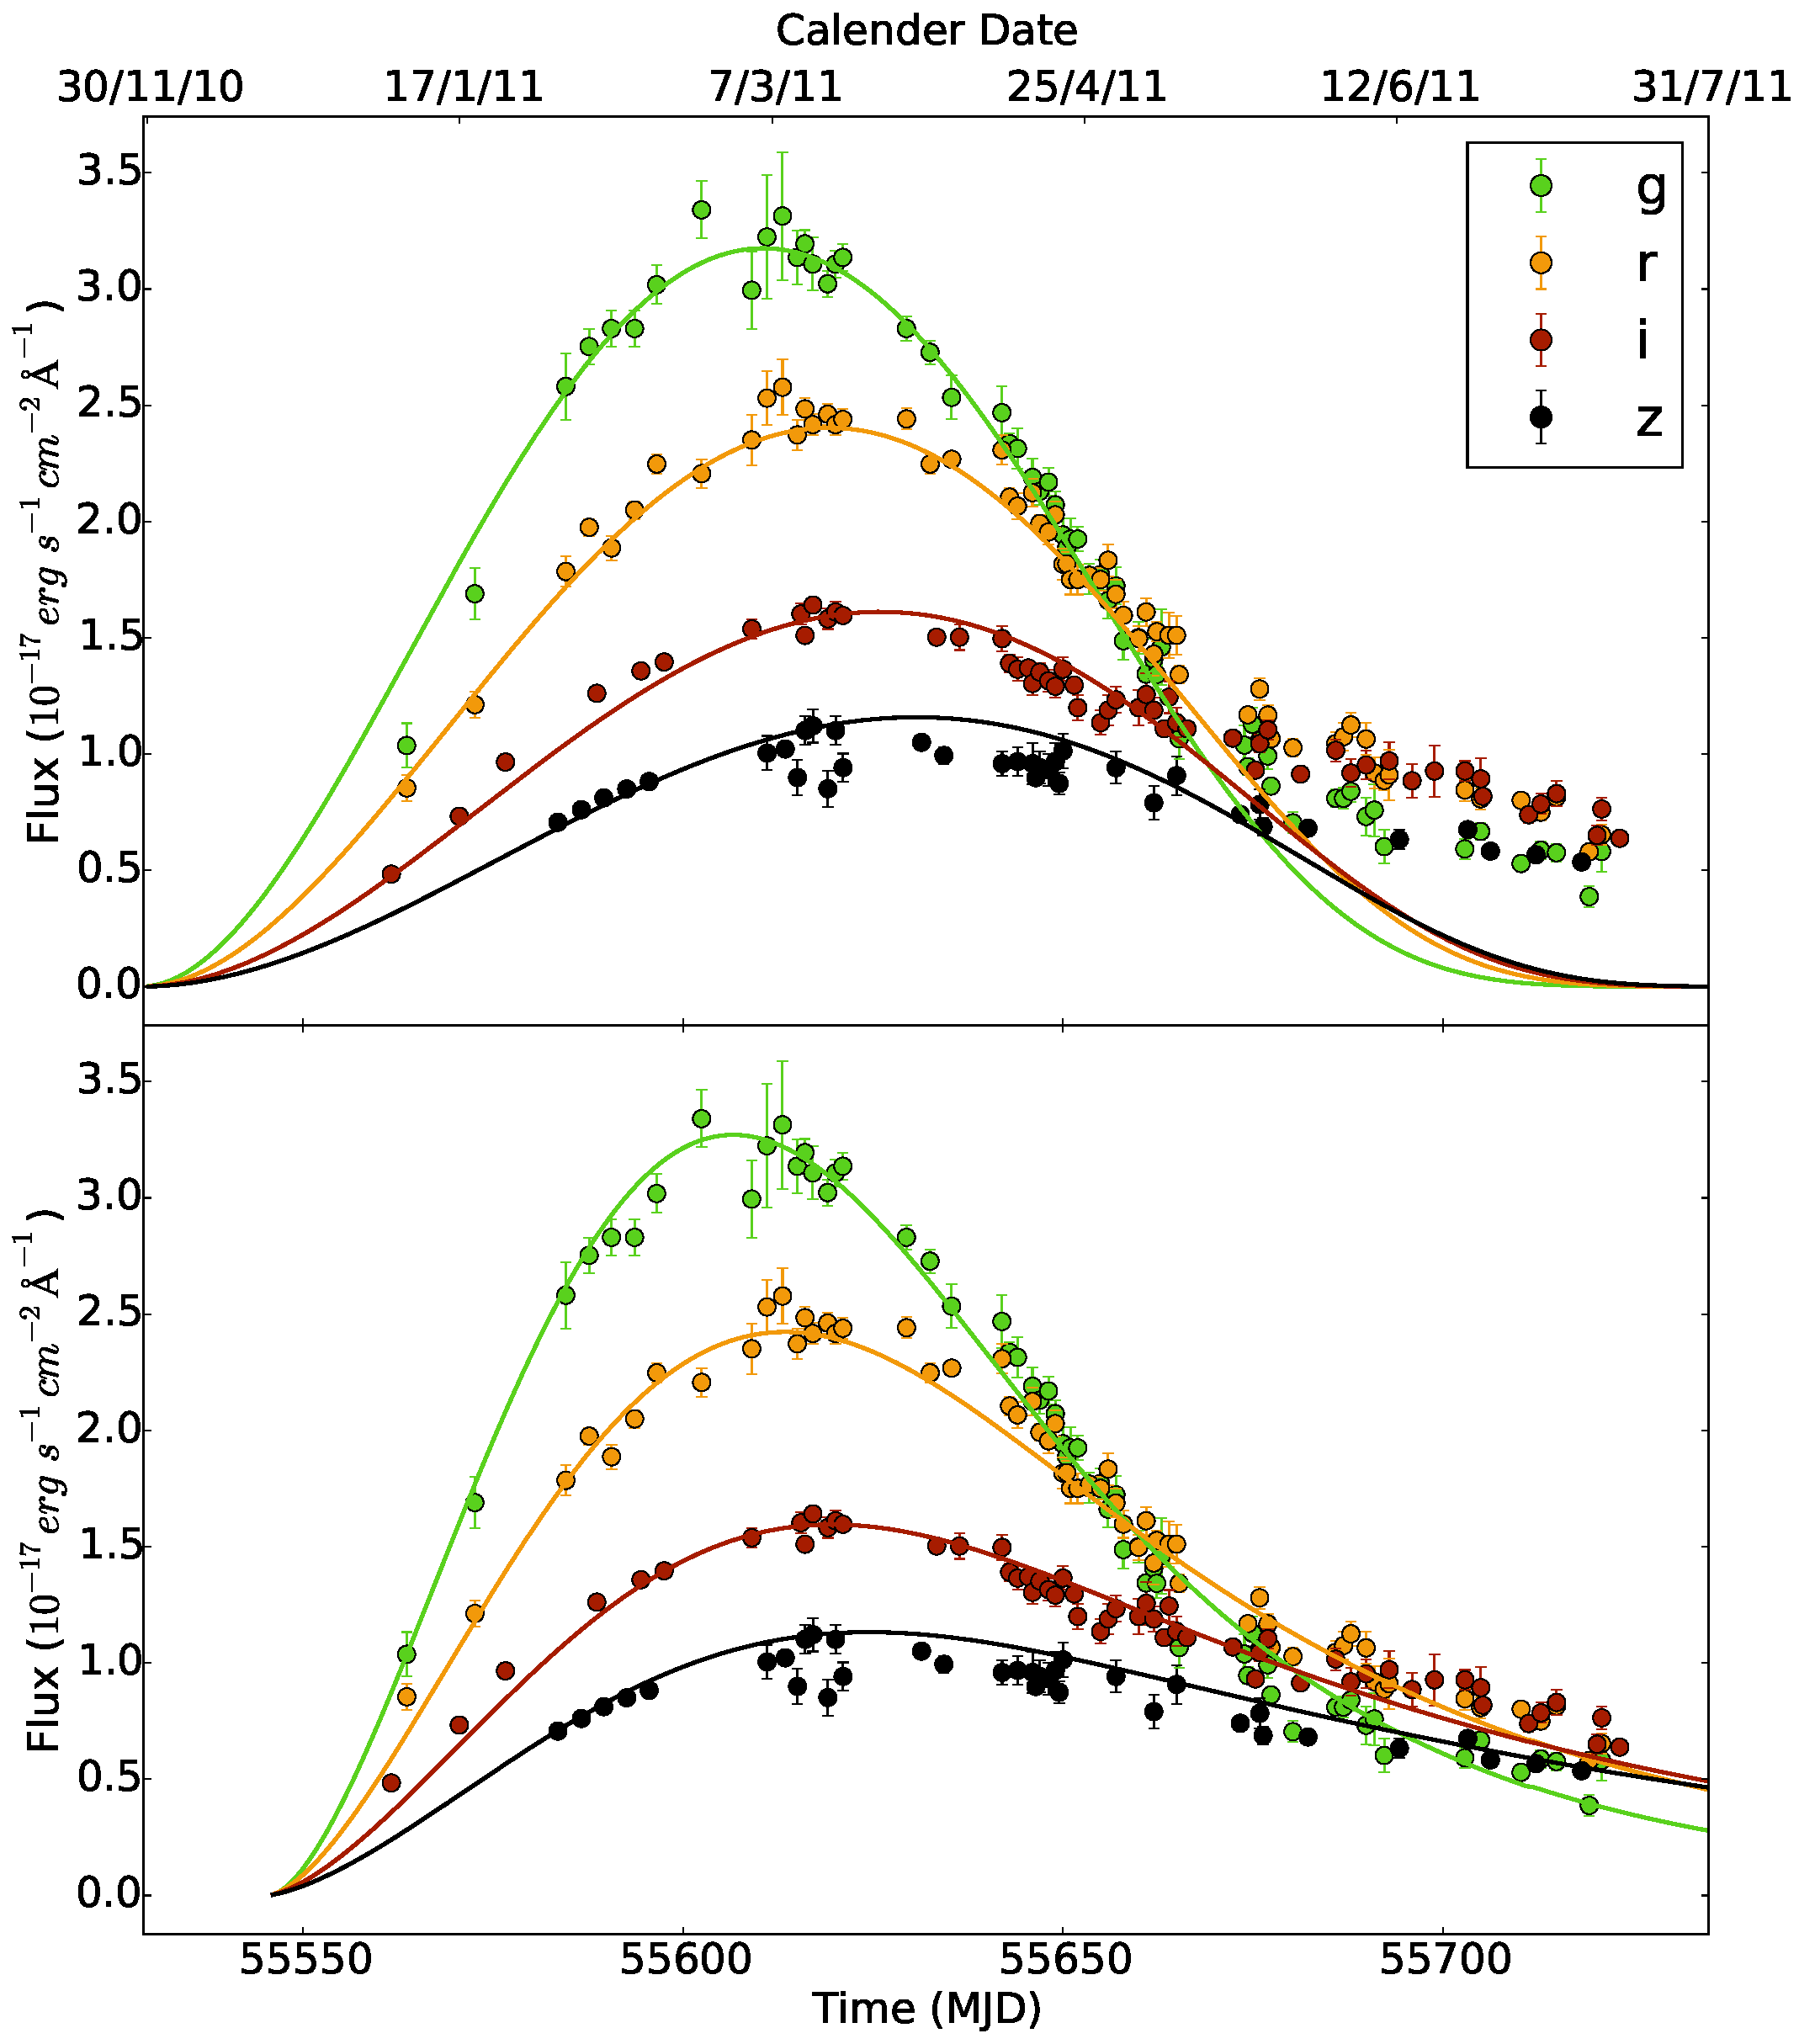
\includegraphics[width=\textwidth]{Figures/Chapter4/BB_Mag_comp}
\caption{The SLSN PS1-11ap $griz$ light curve \citep{2014MNRAS.437..656M} compared to two models describing its photometric evolution. In the upper panel, the model is a simple expanding and cooling blackbody fitted to data around maximum light only, and in the lower panel the model is our `absorbed' magnetar model fitted to the entire light curve. In the case of the magnetar model, the spectrum of SNLS-06D4eu \citep{2013ApJ...779...98H} has been used as an absorption template in the modelling of the SED \sref[see]{sec:KCorrection}). Note that while both models can produce reasonable fits around the peak of the light cuve, the black body model is not able to reproduce the characteristic late-time behaviour of SLSNe. Light curve phases are measured with respect to peak brightness in the rest-frame \textit{u}-band as predicted by our magnetar model fit.}
\label{fig:BB_Mag}
\end{figure}

\subsubsection{Magnetar model}
\label{sec:Magnetar}
To fully capture the evolution of the SED with time we must employ a model for an engine that provides the late time energy deposition needed to explain the photospheric velocity and temperature observed in SLSNe. While still a matter of active debate in literature, in recent years the birth and spin-down of a magnetar model has appeared as the strongest candidate to explain these extremely luminous events \citep{2013ApJ...770..128I,2013Natur.502..346N}. In this model, SLSNe begin as CCSN with a magnetar, a rapidly rotating, highly magnetised neutron star, born at its core. As the magnetar spins down due to the interactions with its environment, it dissipates its energy in the form of high energy radiation that is then captured by the expanding ejecta and thermalised to produce the observed blackbody SED \citep{2010ApJ...717..245K,2010ApJ...719L.204W,2012MNRAS.426L..76D}.

I follow the method from \citet{2013ApJ...770..128I}, based on the Arnett law for the energy diffusion through SN ejecta \citep{Arnett1982}, and the energy radiated by the central engine from \citet{Bildsten2013,Wosley2012}. In order to model the bolometric luminosity, $L$, of a SLSN as a function of time, $t$, we use equation \ref{Eq:MagnetarLum}:
\begin{equation}
L(t) = 4.9\times 10^{46}\,e^{ -(t / \tau_\mathrm{m})^2 }\delta(t) \int_{0}^{t} \frac{2t'}{\tau_\mathrm{m}^2}\,e^{(t'/\tau_\mathrm{m})^2}\,\frac{B_{14}^{2}\,P_{\mathrm{ms}}^{-4}}{\left(1+t'/\tau_\mathrm{p}\right)^2} dt',
\label{Eq:MagnetarLum}
\end{equation}
\begin{equation}
\label{Eq:SDPeriod}
\tau_{p} = 4.7B_{14}^{-2}P_{ms}^{2}days
\end{equation}
\noindent where $\tau_\mathrm{m}$ is the diffusion timescale, $B_{14}$ is the neutron star magnetic field in units of $10^{14}$\,G, $P_{\mathrm{ms}}$ is the magnetar spin period in ms, $\delta(t)$ is the deposition function or trapping coefficient, and $\tau_\mathrm{p}$ is the magnetar spin-down timescale, is defined in \eref{Eq:SDPeriod}, inferred from $B_{14}$ and $P_{\mathrm{ms}}$.

Physically $\tau_M$ is proportional to the ejecta mass($M_{ej}$) which is sometimes chosen as the fit parameter instead. The two parameters can be interconvert using equation \ref{Eq:Mej}, where $E$ is the explosion energy and $\kappa$ the opacity of ejecta.
\begin{equation}
\label{Eq:Mej}
M_{ej} = (\frac{\tau_{M}}{10days})^{4/3}(\frac{\kappa}{0.1cm^2g^{-1}})^{-2/3}(\frac{E_k}{10^{51}erg})^{1/3}M_{\odot}
\end{equation}
\noindent It has been shown \citep{2013ApJ...770..128I,2014ApJ...796...87I,2015MNRAS.452.3869N,2015MNRAS.449.1215P} that the opacity and the explosion energy parameters have only a weak affect the quality of fitting and have therefore been fixed as $\kappa = 0.1cm^2g^{-1}$ and $E = 10^{51}$erg respectively.

The velocity of the ejecta, $v_{core}$ are assumed to be constant and value can be found using the inferred mass of the ejecta, $M_{ej}$ and its kinetic energy, $E_{mag}$ (\eref{Eq:vcore}), which in turn depends on the explosion energy and the energy released by the spin down of the magnetar, shown in \eref{Eq:Emag}:
\begin{align}
\label{Eq:Emag}
E_{mag} = 4.9\times10^{46} B^2 P^{-4} \tau_{P}  \text{ erg} \\
E_k = 10^{51} + 0.5 \times E_{mag} \text{ erg}\\
\label{Eq:vcore}
v_{core} =  \sqrt{\frac{10 E_{k}}{3 M_{ej}}} \text{ cm s}^{-1}
\end{align}

\paragraph{Trapping coofficient}
The trapping coefficient, $\delta(t)$, is defined as the fraction of the high-energy radiation produced by the central engine that gets trapped, and subsequently reproduced as visible light, by the ejecta. It is often assumed in the literature that the trapping coofficient is time-independent and close to unity, implying the full trapping of radiated by the supernova ejecta \citep{2013ApJ...770..128I,2015MNRAS.449.1215P,2015MNRAS.452.3869N}. In this work I use a correction introduced by \cite{2015ApJ...799..107W} with a time-dependent trapping coefficient:
\begin{equation}
\delta(t) = 1 - \exp\left({-\frac{9\kappa \mathrm{M}_{\mathrm{ej}}^{2}}{40\pi  E_k} t^{-2}} \right),
\label{Eq:Wang}
\end{equation}
\noindent where $\mathrm{M}_{\mathrm{ej}}$ is the ejecta mass, $E_k$ is the explosion energy, and $\kappa$ is the opacity. $\mathrm{M}_{\mathrm{ej}}$ is proportional to $\tau_\mathrm{m}$, $E_k$ and $\kappa$ \citep{2013ApJ...770..128I}. We again fix the explosion energy to be $E_k = 10^{51}$\,erg and the opacity as $\kappa =0.1$\,cm$^2$g$^{-1}$.

Using this time-dependent trapping coefficient improves the late-time fit to the light curve. For a typical SLSN we calculate $\delta \simeq 1$ up to 75 days post explosion. However, as the ejecta opacity to high energy photons decreases with time we find $\delta \simeq 0.8$ at 150 days post explosion, emphasising the importance of this correction in the late time light curves.

\paragraph{Deriving Radius and Temperature}
In its simplest form, the magnetar model only predicts the total radiated energy of the SN and does not make any predictions about the SED of the object. It is therefore most commonly used with bolometric light curves, synthesised from the photometry. \citet{2013ApJ...770..128I}, however, shows that it is possible to predict the photospheric radius of a SN based on this model deriving the following equations:
\begin{equation}
\label{Eq:R19}
R(t) = r_{core}(t) \left(\frac{\alpha - 1}{\tau_{core}(t)}\right)^\frac{1}{1 - \alpha}
\end{equation}
\noindent while the radius of the photosphere exceeds that of the core ejecta, and;
\ref{Eq:R20}.
\begin{equation}
\label{Eq:R20}
R(t) = r_{core}(t) - \frac{1 - \frac{\tau_{core}(t)}{\alpha - 1}}{\kappa \rho_{core}(t)}
\end{equation}
\noindent when the photosphere recedes into the core. $r_{core}(t)$, $\rho_{core}(t)=$ and $\tau_{core}(t)$ are defined as follows:
\begin{align}
r_{core}(t) = v_{core}  t \\
\rho_{core}(t)= \frac{3 M_{ej}}{4  \pi  r_{core}^3(t)}\\
\tau_{core}(t) = \kappa  \rho_{core}(t) v_{core} t
\end{align}

Combining this with the total luminosity and assuming that the object radiates as a uniform, spherical blackbody gives us the photospheric temperature. This can be injected into the Planck law to give an approximation for the SED of a SLSN. This method allows for the magnetar model to be fit directly to the multi-band photometry without the need to produce the pseudo-bolometric light curves. We combine this with the absorption templates to produce a model of the SLSN spectral evolution as a function of time.

\subsection{SLAP}
Upon establishing an approach for modelling SLSNe it was important to encapulate it in a software package capable of performing under a number of situations. In this thesis the magnetar model was used in fitting the light curves of both known SLSNe and a variaty of transients, the majority of which could not be well approximated using this model. We have also used it in simulating SLSN in SNLS as well as producing an artificial training sample for the DES machine learning study of SLSNe.

The code was required to satisfy the following requirements:
\begin{itemize}
  \item Fit the magnetar model to all literature SLSNe and estimate their parameters.
  \item Perform a succesful fit to any light curve and return an output, regardless of whether it is physical.
  \item Move the object to any redshift within the range of SNLS and DES.
  \item Allow for the use of any spectral template.
  \item Allow for extensions and modifications to the magnetar model.
  \item Simulate SLSN light curves given input model parameters.
  \item Plot the data and the model, allowing for model comparisons.
  \item Fit light curves on the time scale of minutes and simulate with subsecond performance.
\end{itemize}

The performance requiremets were based on our need to fit the entire archival sample of transients from SNLS as well as regularly fit the live DES transients with an aim of searching for new SLSN candidates. At an average DES cadance of $\sim$5\,days it was necessary that the fitting is performed at a shorter timescale. Similarly, the studies of the rate of SLSNe \cref{Chapter3} and the ML search for SLSNe \cref{Chapter5} required millions of SLSN light curves to be generated for each iterations of the experiment.

After initially testing the model and the fitting methods in the \textsc{Python} langauge environment, I have developed a package that satisfies all of our requirements: The SLSN Lightcurves Analysis Package (SLAP). Written in a combination of \textsc{C++}, \textsc{Cython} and \textsc{Python}, it was used in every project undertaken as part of this thesis. The use of C++ and a number of optimisation techniques allowed for a very large performance improvement versus a similar \textsc{Python} package. \textsc{SLAP} performs model fitting in $\sim$40\,s for an average SNLS light curve and simulated a SLSN in $\sim$10\,ms. The package was published as part of my study of the rate of SLSNe in SNLS \citep{Prajs2016}.

\subsubsection{Code design and structure}
SLAP was designed as a modular, reusable and extendable package while at the same time heavily focussing on the the run-time performance of the code. I have heavily relied on the concepts of Object Oriented Design and Polymorphism to allow me to implement any model as a an extension to the code. At the core of \textsc{SLAP} I have used the concept of approximating the SED of SLSNe as absorbed black bodied. I have defined a virtual \textsc{Model} class that acts as a base class that defined the method for calculating an SED based on the temperature and radius of a SN photosphere. This class is then inherited by a model that defines the time evolution of the SED. This allowed me to use a number of extensions to the base magnetar model that were implemented as plug-ins.

\subsubsection{Model extensions}
While the base magnetar model is a good fit to the majority of SLSNe light curves, in some cases, such as DES14X3taz, it is impossible to fully model the SN without introducing any further assumptions. In this section I will describe a number of magnetar model extensions which I have introduced in order to improve the quality of our fits. It is important to note that these were never used in the simulation of SLSNe for both the rates of SLSNe in \cref{Chapter3} nor the creation of the DES artificial training sample in \cref{Chapter5} as the base model remains a good fit around the maximum light which, in case of the DES and SNLS seasons, is the region observed by our data. The extensions demonstrate the capabilities \textsc{SLAP} and were used only to broaden our understanding of specific, individual objects.

\paragraph{\citet{Piro2015}}
Upon the discovery of DES14X3taz, the question of the engine powering the pre-cursor bump was an important one to answer. \citet{Smith2016} showed that the peak is well explained by a model wherein the supernova explodes inside of an envelope of an extended dense wind. The shock-breakout which is usually observed as a short, $<$1\,day, flash of high energy radiation gets reprocessed into a longer duration emission of lower energy radiation. This model is highly degenerate in the ejecta mass and explosion energy. However, as these parameters also play part in the modelling of the spin-down of a magnetar, the combination of these two models gave us an unprecedented opportunity to derive these parameters directly from the observed data.

In this version of the model, we intoduce a new free parameter, t$_d$, measuring the delay between the explosion of the SN and the onset of the magnetar spin-down. These have not been previosly considered to occur at different times \citep{Nicolls} as there are currently no models that require a delay between the supernova explosion and the formation of the magnetar [ME: NEED TO CHECK THIS, THERE MIGHT BE A PAPER BY WOOSLEY]. However, I have found through the modelling of DES14X3taz that it is impossible to reconcile the magnetar and extended shock models without the introduction of this parameter. Further evidence for is presented in \cref{par:R0nonzero} where the best fit magnetar model for DES14X3taz is shown to require an extended photosphere, consistent with a t$_d ~\sim$ 17days (assuming a constant explansion velocity), in order to better describe the rise phase of the SN.
[ME: MAKE A PLOT FOR THIS]

\paragraph{R$_0~>$ 0}
\label{par:R0nonzero}
While it is widely believed that the birth and a spin-down of a magnetar the most likely progenitor for SLSN, the exact process through which the high-energy radiation produced by the magnetric breaking is transported into the outer shells of the ejecta is not yet understood. If the injection of energy does precisely coincide with the time of explosion of the progenitor star, the SN could go though a "dark" phase followed by a rapid rebrightening. In several cases, including PS1-11ap and DES14X3taz (where we exclude the pre-peak bump data), the magnetar model does not fit the earliest stages of the light curve correctly.

In order to investigate this delay, I have introduced a non-zero initial radius of the progenitor. While the radius of the progenitor star is never null, it is usually negligible in comparison with the expansion velocity of the ejecta. However, in the case of DES14X3taz and PS1-11ap, I found initial radii consistent with ejecta that underwent an expansion at a constant velocity for 17 and XX days respectively. PS1-11ap has no observations prior to its first detections making it impossible to determine if the object was associated with a pre-peak events. This technique, however, can provide insight into the mechanism behind the magnetar energy injection even in the absence of the earliest and pre-explosion epochs. [ME: MAKE A PLOT FOR THIS TOO]

\paragraph{Nickel decay}
Another intersting questions that we were able to investigate using \textsc{SLAP} is the contribution from the radiactive decay of Ni56 and Co56 as an additional energy source powering the ejecta. I have introduced this to investigate a potential mechanism powering the peculiar, flat evolution of DES13S2cmm. In this model, I add the contribution from the decay of these radioactive elements into the bolumetric luminosity of the SN and do not introduce any other modification to the model. While we find that the radioactive decay alone cannot account for the evolution of DES13S2cmm, this test demonstrated the easy with which we are able to modify our models to test new assumptions. The evolution of DES13S2cmm is further investigated in Angus (in prep).

\subsubsection{Maximum Likelihood methods}
The success of \textsc{SLAP} in fitting SLSNe cannot be attributed only to our work on the models but, perhapse in the largest part, to the optimisations applied to the fitting routines. One of the main goals for \textsc{SLAP} was a full autonomation of the fitting process, without the need to manually fine-tunning any input parameters. This is crucial performing fits on large datasets, containing thousands of objects where only a small fraction are likely to be good matches to the model. Furthermore, we do not wish to intruduce any human biases to the fitting procedure, particuarly in the case of the ML training sample as the techniques used by us are sensitive enough to recover such biases over the true trends in the data.

In the early testing phases of the project we have explored fitting the model using the Maximum Likelihood Estimate (MLE) method. This approach is based on maximising the Likelihood function which, in the frequentist approach, describes the probability of the observed data originating from the underlying model. As the uncertainties on our observations are normally distributed I use the Least Squares (LS) regression analysis which is a special case of MLE. In LS fitting, we minimise the residual, defined as the uncertainty weighted difference between the data and a model, using the $\chi^{2}$ test as a metric for defining the goodness-of-fit:
\begin{equation}
  \chi^2 = \sum\limits_i^N \left( \frac{O_i - m_i}{\sigma_i} \right)^2
\end{equation}

\paragraph{MPFIT} \label{sec:MPFIT}
The MLE fitting approach was implemented in \textsc{SLAP} using \textsc{MPFIT} [CITE], based on \textsc{Fortran}'s well known package \textsc{LMFIT} [CITE]. \textsc{MPFIT} is an implementation of the Levenberg–Marquardt non-linear LS fitting algorithm. This is a popular and highly optimised example of the class of iterative, gradiant descent algorithms that work by traversing the likelihood function, moving in the direction of lower $\chi^2$ (i.e. higher likelihood). The algoriths use a gradient (either analytical or numerical) of the likelihood function to inform the direction and size of a jump taken at each iteration. In the Levenberg–Marquardt algorith a damping coefficient is introduced decreasing the number of steps taken by the algorithm before converging on a minimum.

While \textsc{MPFIT} was very promising during our testing, we discovered that the quality of our fits strongly dependant on the choice of the initial parameter guesses. This is a common issue amongst all gradient descent algorithms informed only by the gradient at the measured point. This leads to them finding the local likelihood maximum, nearest to the initial parameter guess instead of the global value. This contradicted one of our strongest demands for the package, as \textsc{SLAP} would require manual modification for the initial parameter guesses, making it impossible to use with a large number of objects.

\subsubsection{Bayesian Inference}
While a number of global optimisation approches have been trialed, we realised that the complexity and degeneracies of the magnetar model require a full Bayesian treatment in order to efficiently find the global minimum (or Maximum Likelihood) of the model. Bayesian Inference is a technique based on the Bayesian view of probability, derived from Bayes' Theorem which states that for a set of model parameters $\mathbf{\theta}$ and data $\mathbf{D}$:

\begin{equation}
  P(\mathbf{\theta}|\mathbf{D}) = \frac{P(\mathbf{\theta}) P(\mathbf{D}|\mathbf{\theta})}{P(\mathbf{D})}
\end{equation}

\noindent where $P(\mathbf{\theta}|\mathbf{D})$ is the Posterior Probability, $P(\mathbf{\theta})$ denotes the Prior Probability, $P(\mathbf{D}|\mathbf{\theta})$ defines the Likelihood and finally, $P(\mathbf{D})$ is the model Evidence.

The Posterior Probability describes the probability of the model $\mathbf{\theta}$ given the observed data $\mathbf{D}$. The biggest difference between the frequentist and bayesian view of probability is the inclusion of the Prior Probability which describes our believe in the model before we make the observations $\textbf{D}$. The Likelihood function here is analogous to the Likelihood function used in MLE. In fact, in the special case where the Prior distribution is uninformative (i.e flat), Bayesian Inference is equivalent to MLE and would yield the same result. The Evidence, $P(\mathbf{D})$, acts as a normalisation constant and is only used in comparing distinct models and not in determining their "best-fit" parameters. $P(\mathbf{D})$ is usually very difficult to computer as it requires the Likelihood function to be intergrated over the entire parameter space. The following two paragraphs describe the methods I used to compute the Posterior Probability distribution as well as estimate the model Evidence.

\paragraph{MCMC}
Markov chain Monte Carlo (MCMC) is an extremely popular and widely used set of techniques for estimating the Posterior distribution. One of its simplest implementations, the Metropolis-Hasting algorithm, iteratively samples the Posterior distribution by drawing a new point from the normal distribution centered at the previous parameter and accepts it if the value has a higher probability. However, what differenciates the MCMC approach from MLE techniques is that a sample can also be accepted if it has a lower porbability that the previous point in the chain. The acceptence ratio here is defined as the ratio of the new probaility to that of the previous iteration. This allows the 'walker' to sample the entire Posterior Probability distribution provided that the chain a sufficiently long chain is computet.

In this thesis I have tested both a custom MCMC implementation as well as the popular and heavily optimised, multitreated package, \textsc{Emcee} [CITE]. While both approaches can estimate the Posterior distriburions as well as the best-fit parameters with no external input or hyperparameter finetuning, their performance based on a need to evaluate millions of models to provide a full sampling of the Posterion distribution, was however very poor. A light curve fit would often require in excess of 8 CPU hours, despite the heavy optimisations of the model.

\paragraph{\textsc{MultiNest}}
A recently developed technique for approximating the Posterior Probability distribution, showing a great improvement in efficiency is Nested Sampling [CITE]. Here, the Posterior distribution is calculated as a by product of the model Evidence evaluation. While this is usually a very computationally expensite calculation, Nested Sampling used the properties and relationship between the likelihood and the prior reduces the multi-dimentional integral into a single dimention, which is much simple to evaluate. The algorithm populates the prior with a relatively small (I used 2000) 'live' points which calculate the Likelihood. The point with the lowest Likelihood is replaced by a new point, geometrically closer to the point of highest Likelihood. The new point is accepted if its Likelihood is higher than the point it originally replaced. Nested sampling provides a near 1000-fold efficientcy improvement over the common MCMC methods. This makes this approach fast and robust enough to satisfy the designrequirements of \textsc{SLAP}.

In this thesis, I use \textsc{MultiNest} [CITE], a Fortran based implementation of the Nested Sampling algorithm. This is one of the most popular implementations of the technique. Its robustness and performance tested and demonstrated in a number of cosmological studies using the CosmoMC package [CITE], making it the perfect package for us. On of the greatest advantages of \textsc{MultiNest} is its operation in a multi-modal mode where the algorithm returns not only the Maximum-a-Posteriori (MAP) parameters but also positions of other, local, maxima. [SHOULD I PUT AN EXAMPLE CHAIN/CORNER PLOT HERE?]

\subsubsection{pyMagnetar}
While SLAP was very heavily used thoughout this thesis as a tool for modelling SLSNe, putting an emphesis on the optisations involving model fitting, I have also used it as a tool for building synthetic cataloges of SLSNe. While this was directly possible from within the C++ frontend, it is difficult and inefficient to interface the code with the majority of modern astronomy pipelines which are most commonly written in \textsc{Python}. Using the \textsc{Cython} language, I have created a higher level interface to the code named \textsc{pyMagnetar} [EXPAND OR DELETE].

\section{Modeling CCSN}
In recent years there is an increase in interest in modelling of CCSN. This very heavily driven by the arrival of very large surveys such as LSST.

--- This is mainly driven by the attempts to use Machine Learning for classification of SN in large surveys such as LSST
--- Previous templates were not very good as they only included a few objects
--- The best templates are Kessler10 used to create a sample of CCSN for the SPCC which produced a sample of 2000 SN including SNIa anCCSN and is widely used as a training sample for SN Machine Learning projects, this is not enough. There were only 3 SNIb in the whole sample!

- Things that we needed to change to make better templates
--- Use all the latest data
--- Extent the spectra
--- Don't interpolate the Toyah

In this section I will describe the main design choices behind both CoCo and pyCoCo, discuss the models used in modelling the light curves of CCSN as well as those undertaken to create their spectroscopic templates. I then describe the steps taken to extend out spectroscopic templates into both the UV and IR parts of the SED not observed by the spectra.

\subsection{\textsc{CoCo}}
In many way the package I have developed for simulating CCSN is very similar to \textsc{SLAP}, used for modelling SLSN. Its performance was, again, a critical part of the code design as we aim to similate millions of light curves in LSST and DES. This has lead to our decision to again follow the principle of developing the core of the package in \textsc{C++} and using \textsc{Cython} to create a \textsc{Python} front-end interface. I will follow our internal naming for the packages and refer to the backend packages, developed in \textsc{C++}, as \textsc{CoCo} and the \textsc{Python} front-end wrapper as \text{pyCoCo}.

\textsc{CoCo} consists of four core packages, \textsc{LCFit} used to fit the SN light curves with a number of models, \textsc{SpecFit} used to match the observed spectra to the photometry, \textsc{SpecPhase} which assigns the phase to each spectrum and corrects them common redshift and finally \textsc{LCSim} which simulated SN based on the outputs of the previous three packages. In the following subsections I will describe this packages as well as the models, decisions and assumptions we made that led to the final product.

\subsubsection{\textsc{LCFit}} \label{sec:LCFit}
The process of creating the templates for CCSN by fitting the observed light curves with an analytical model able of describing their morphology as well as reliably extrapolating them. We need this in order to, in later steps, flux calibrate the observed spectra to match the photometry. The interpolation allows us to calibrate the spectra on epoch where there were no photometric observations. While a non-parametric aproach could be used such as Spline Interpolation or Gaussian Processes we needed the required the ability to extrapolate the light curve fits beyond the range of the observed point in cases where the spectroscopic follow either exceeded the photometric follow-up or, in even rarer cases, predeeded it.

At this phase of the procedure, the models are fitted using the \textsc{MultiNest} fitting routine. We followed a similarly route to \textsc{SLAP} giving us the state of the art fitting accuracy and reliability. The photometry is fitten individual for each band ... [WRITE MORE HERE ABOUT THE OUTPUTS]

We have trialed and implemented a number of models thoughout this projects.

\paragraph{Bazin09}
The simplest, yet the most versatile, model for describing CCSN can be found in \citet{Bazin2009} (Bazin09 from here on). This simple model is a combination of a logistic function which describes the rise of the SN and an exponential decay which matches the decline of the light curve (\eref{eq:Bazin09}). This model was succesfully used to photometrically identify CCSN-like events in the SNLS. While the simplicity of the model means that it is not able to fully describe the behavious of all SNIb/c, it provides a good match to those dominated by the radioactive decay of Nickel56 as their power source. [WRITE MORE]

\begin{equation}
\label{eq:Bazin09}
  F(t) = A \frac{e^{-\frac{t - t_{max}}{\tau_{fall}}}} {1 + e^{\frac{t - t_{max}}{\tau_{rise}}}}
\end{equation}

\paragraph{Kessler10}
A more complex version of the model used in \citet{Bazin2009} was used in \citet{Kessler2010} (Kessler10) as a base for their work on creating a photometric sample of CCSN for the use in the Supernova Photometric Classification Challege. While the model parameterises SN using an underlying exponential decay and rise, it additionally provides the ability for the model to account for a secondary maximum often observed by SNIa. While their motivation behind this modification was mainly the modelling of SNIa and CCSN using the same model, the additional feature behaves differently in these distinct classes of SN. As CCSN rarely show signs of a seconadary maximum, the extra dgrees of freedom often improve the early fits around the early rise time phases of the SN where there are often other mechanism (shock breakout, Hydrogen recombination ect.) That inject additional sources of energy into the light curve.

One of the drawback of this model, and the reason why we have not found it to improve the quality of our fitting is the common timescale behind the decay of the primary and secondary maxima. This is likely motivated by the physics of SNIa, but does not correspond to the observed behavious in CCSN where the power sources are not physically linked and therefore act on different dynamic timescales.

\begin{equation}
  F(t) = A \times [1 + a_1(t - {t_0}) + a_2(t - {t_0})] \times \frac{e^{-\frac{t - t_{0}}{\tau_{fall}}}} {1 + e^{\frac{t - t_{max}}{\tau_{rise}}}}
\end{equation}

\paragraph{Karpenka12}
\citet{Karpenka2012} (Karpenka12) further improves on the model found in Kessler10 by decoupling the onset of the primary and secondary peak. While retaining the same number of free parameters as Kessler10, the improvements in the fitting quality is considerable for the SNIb/c with a more complex morphology.

\begin{equation}
  F(t) = A \times [1 + B(t - {t_1})^2] \times \frac{e^{-\frac{t - t_{0}}{\tau_{fall}}}} {1 + e^{\frac{t - t_{max}}{\tau_{rise}}}}
\end{equation}

This model was successfully used in a project involving SN photometric classification using basic Neural Networks \citep{Karpenka2012}, demonstrating that it is a suitable model for our use.

\paragraph{Firth18}
Finally the last model considered by us in this study is based on the Karpenka12 model but adds an aditional, independant of other properties peak which helps to model the shock breakout observed in some supernova

[WRITE THE EQUATION HERE]

This model has too many free parameters and can only be used on light curves with a lot of data point and those that have a very well defined shock breakout otherwise the extra degrees of freedom simply act as an aditional degeneracy in the modelling.

\subsubsection{\textsc{SpecFit}}
One of the most crucial parts of our procedure for generating the CCSN templates is matching the observed spectra flux to the photometry. It is commonly assumed that due to the complexity of flux calibrating spectra they are only correct to within 10\% accuracy. While in most studies this accuracy is often not an issue as other factors contribute larger errors, in the case of the DES and LSST SN simulations this accuracy is significantly below the precision of the photometry. The process used to correct the flux calibration, refered to as spectral 'mangling', adjusts the spectrum such that the synthetic flux measured by passing the spectrum though filter response functions matches the observed photometry. I have excapsulated this in the \textsc{SpecFit} package.

In order to adjus the spectrum we multiply is my a spline function designed in such a way to smoothly move the flux in different parts of the spectrum. A spline is a smooth, continuus function defined using a number of control points defined using a position and amplitude. The wavelength at which we place the control points matches that of the central wavelength of the filters while the amplitude is determined using minimisation. We again use \textsc{MultiNest} for the fitting here. The choice of the end points of the spline are important and were places at 100\AA outside of the wavelength range of the mangled spectrum. The ampltude of these points is not subject to the fitting, instead they are determined by extrapolating two most extreme points on either side of the spectrum using a straight line.

While developing the mangling code we have discovered several issues which neeeded to be addressed in order to produce reliable results. One of the major issues arose due to control points of the splines laying to close to each other, causing the interpolated function to behave eratically and far from the expected. We have traced this to using filters which are derivatives of each other, such as Johnson's R and SDSS-\textit{r}, that only vary in central wavelength by $\sim$50\AA. This should not be a problem if the control points were already calibrated but due to the nature of the fitting process, the points were fit independantly meaning causing huge, non-linear degeneracies that not even \textsc{MultiNest} could cope with. We were therefore force to remove the overlapping spectra from the mangling. As we were mainly focusing on preserving a maximum amount of information in the blue parts of the spectrum we have retained the band with a lower central wavelenth.

Furthermore, we have found that the mangling is not reliable when less than three bands are used to set the control points. This is caused by the end points being extrapolated using the previous two points. Spectra which only overlapped with two distinct bands could therefore not be used as the control points used for the extrapolation were the same for the upper and lower bands, causing degeneracies that were difficult to handle with even suphisticated fitting routines. As a final product, \textsc{SpecFit} saves the flux calibrated spectrum in the ASCII format, scaled to the observed photometry and is not redshift (or otherwise) corrected.

\subsubsection{\textsc{SpecPhase}}
A major difference between my approach to fitting the SLSNe and CCSN if the treatment of their explosion date (or start date). In the case of SLSNe we have a well defined explosion date, set as a free parameter in our model, prior to which we can assume the flux to be null. In the case of the models in \sref{sec:LCFit}, their rise is not abrupt but following a logistic function which only tends towards zero at negative infinity making it impossible to define the explosion date without adding extra assumptions.

We must therefore define the time at which we insert the light curve in our simualations using a different system. In this case, we use the time of the maximum light of the SN as the point of reference, measured in the rest-frame V-band. The phase is determined in the following way; the spectra are shifted to z=0 (rest-frame). Using the distance moduli for the host galaxies obrained from the NED archives [CITE] I scale the flux for each spectrum to give their apparent flux at 10pc (e.g the absolute magnitude). I then synthesis a V-band light curce from the spectral time series and fit it using the same approach as in \sref{sec:LCFit}. The peak is determined numerically as the maximum of the light curve fit. As a final result the package returns a list containing the phase relative to peak for each spectrum found for the object as well as a spectral time series normalised to z=0 and absolute magnitude of the SN.

\subsubsection{\textsc{LCSim}}
Following the previous steps we can obtain a set of spectral templetes that can now be used to generate a new sample of synthetic SN light curves. This step is based on the same concept as \textsc{SpecPhase} used to determine the phases of the template spectra. The template spectra are shifted to the required redshift and corrected for the distance modulus. The spectra are also corrected for the host galaxy extinction before they are redshifted as well as the milky way extinction once at the observed redshift. Synthetic photometry is them generated for the requested bands before a light curve model is fit to allowing for generating simulated photometry points at an arbitrary phase.

This is the only part of the whole package that does not rely on \textsc{MultiNest} as the tool minimisations. While it would have been optimal from the accuracy and robustness point of view to use it, we have found that its performance was insufficient in order to allow us to simulate millions of CCSN. After discovering issues with numerical instabilities in \textsc{MPFIT} (used in \sref{sec:MPFIT}) when computing the derivative of our residual function, we have decided to use a more modern package, \textsc{Minuit2} [CITE]. Designed by CERN and heavily used with in the ROOT library [CITE], \textsc{Minuit2} utilises more modern numerical libraries which helps it to handle numerical uncertainties better than its \textsc{Fortran} derived predecesors. \textsc{Minuit2} implements a number of algorithms derived from the broader gradient descend family. In \textsc{LCSim} we use \textsc{migrad} which is the default minimiser in the package and is based on the same concept as the Levenberg-Marquardt algorith used in \textsc{MPFIT}.

\subsection{pyCoCo}
Following the same design patern as in \textsc{SLAP}, I have created a \textsc{Python} interface for the \textsc{LCSim} package using the \textsc{Cython} intermediate language. The ability to iterface the code with \textsc{Python} allowed me to manipulate the simulated light curves directly in the memory without the need to create a time and memory consuming intermediate output, significantly reducing the overheads in the simulation. This also simplified the process of storing the final simulations by interfacing the output directly with a \textsc{PostgreSQL} database.

As the package was always intended for a wider audiance, not limited purely to this project, \textsc{pyCoCo} forms a simpler and more approachable interface to \textsc{CoCo}. Furthermore, Firth et al. (in prep) has build a large suite of wrappers and tutorials for template generation which compliment \textsc{pyCoCo} and allow for the whole procedure to be performed directly from \textsc{Python}.

\subsection{SNIb/c SED UV Extensions}
SNIb/c were the main focus of \textsc{CoCo}. Their simulations are some of the most desired amonsts various classes of SN as they are the main source of contamination in the samples of SNIa due to the similarities in the physics that powers their luminosity. SNIb/c are, however, relatively rare in comparison to SNIa or even hydrogen-rich SN.   Firth et al. (in prep) collected a sample of 'good' SNIb/c lightcurves and their respective spectra from the literature. 29 SN were part of the initial sample before extra quality cuts (described in [CITE SECTION]) were appplied. The final sample included 17 SN that were used to generate the templates. This sample is larger than that created by \citet{Kessler2010} and included SN from the pre-SDSS era to latest objects observed by iPTF.

As could be extected in such a diverse sample of objects, a large number of the spectra do not have a very good wavelength coverage, often not exceeding the range of 4000-7000\AA. On a contrary, the light curves for almost all SN in the sample include the minimum of BVR bands with a number of obsects including both redder and bluer bands. It was therefore possible to use the extra light curve information as a base upon which we can extend the spectroscopic templates of the SNe. Red extensions were required in order to simulate the low redshift SN in the reddest bands (e.g. DES \textit{z}-band). These extensions were performed as part of Firth et al. (in prep) and used the black body equation to extend the spectra up to 10500\AA. The flux was then corrected to the photometry by again passing the time series though \textsc{SpecFit}.

In contrast with the red extensions, in the UV extensions we could not rely on the observed photometry. As we aim to simulate SNIb/c to redshifts of up to z$\approx$0.8 in the DES deep-fields, we require the templates to extend to $\sim$2000\AA in order to overlap with the observer-frame \textit{g}-band at that redshift. The required region of the light curve most closely matches that of the Swift-UVOT UVW1 filter [CITE]. The Swift satellite launched in late 2004 as a rapid response Gamma-Ray Burst (GRB) detector. Since then, it has observed a number of SNIb/c, giving us a glimpse at their UV light curves. The data, however, is not present for all objects rising a need to approximate the behaviour for the objects with no UV data.

Using the data collected by the Open Supernova Catalogue (OSC), I have created a subsample of our template SNe with available UV data. Amonst these, a large number of obsects only included the very earliest epochs likely triggered as a follow-up based x-ray detections for the object. A number of objects later received an extended follow-up campaign that gave us the light curve information past maximum light. For this objects, I have performed light curve interpolatin using Gaussian Processes (\cref{sec:GP}). This allowed me to compare the UVW1 light curve to the V-band, as shown in figure \fref{fig:VvsUVW1}. This showed that during the main phase of the SN (excluding the shock breakout), the UWV1 and V band light curves followed a very similar evolution. The UVW1 showed to be 2.5 magnitude dimmer (10 times dimmer in flux). I therefore use this property to create artificial UVW1 light curves by offsetting the V-band light curve by 2.5 magnitudes in flux and retaining its overall evolution.

\begin{figure}
  % \includegraphics{/path/to/figure}
  \caption{The ratio between the UVW1 and V band filters plotted for a number of stipped envelope SNe.}
  \label{fig:VvsUVW1}
\end{figure}

Using the extended light curve coverage we can extend the spectra in the same way as we did with in the case of IR. As there is little information about the spectral evoution of CCSN, I follow the same technique as Firth et al. (in prep) by using a black body to extend the SEDs. We then again pass the extended spectrum though \textsc{SpecFit}, matching the spectrum to the syntheric UVW1 filter.

\subsection{SNII with CoCo}
The aim of Firth et al. (in prep) was predominanty to generate a sample of SNIb/c in order to study and classify the samples of SNIa for cosmological studies. While we knew that our approach should be able to tackle SNII in a similar analysis, this was never attempted as part of Firth et al. (in prep) and instead was performed only as part of this thesis. In large, I have followed the same methodology excluding several steps that were optimised to better suit hydrogen rich SNe or improved based on the lessons we have learned in Firth et al. (in prep). This also gives me an opportunity to describe the steps taken to produce the sample of spectral templates in a project similar, but performed independantly, to Firth et al. (in prep).

All data in this project was obtained using the Open Supernova Catalogue repository. The data was collected for objects matching the hydrogen-rich SN classes including: SNII, SNIIP, SNIIL, SNIIn, SNIIb and SN1987A-like. Only objects with a light curve covering the pre-peak and post-peak data as well as a relatively dense spectral coverage covering the same regions were included in the sample. I have used the toolkits developed in Firth et al. (in prep) to nightly average any spectra that were taken in rapid succession. I have also removed the regions of each spectra where no supernova light was detected or the noise was too large to confidently recover the underlying morphology of the SED.

In the next step, I have removed all spectra with a coverage shorter than two photometric bands. I have also removed the spectra that did not overlap with the V-band. Following this clearing stage, I have removed all objects that no longer satisfied the coverage required for our analysis. This has retained a sample of 11 objects that can be used as templates.

The light curves for all remaining objects were then fit with all models described in \sref{sec:LCFit}. While, due to the increased number of degrees of freedom, the more complex models such as Karpenka12 and Firth18 are able to fit the data more precisely, they are unable to constrain light curves will a small number of epochs. Unfortunately, in the process of simulating the light curves we fit the models to photometry synthesised from the spectra which is sparse for most objects in our sample. Instead of using the more complex models, I fit all SN in the sample with the most basic Bazin model. Despite its lack of complexity it has produced a good fit all light curves in our sample. I must note here that this was not an expected result. SNIIP are associated with a light curve platoe phase which could not be accounted in this model. However, none of the objects that observe this behaviour had sufficient spectral coverage to pass the previous quality cut. This is not an optimal scenario as a whole class of objects are, seemingly, excluded from the sample. The platoe is, however, more prominant in the redder bands and therefore does not appear as a strong feature in the rest-frame blue bands that form the majority of the observed SED at high redshift where we will be simulating the majority of our SNe.

One mayor difference between the work undergone on SNII and SNIb/c in Firth et al. (in prep) is the treatment of the spectra before \textsc{SpecFit} is used to apply the mangling step. In Firth et al. (in prep) we excluded all spectra that did not have a sufficient wavelength coverage to successfully undergo mangling. We found that objects with a coverage shorter than three filters were not able to constrain the correcting spline function. In many cases the spectra were only short of few hundred Angstrom, most often in the red part of the spectrum. Instead of removing such objects, I linearly extrapolated the final 100\AA of the observed spectra to the wavelength required to complete the third filter coverage. This helped me to retain a much larger number of spectra, in some cases saving the object from being removed from the sample under my quality cuts.

Another major difference between the projects is the approach to extending the light curves in both the IR and UV. In the IR, I have found that a number of objects, pre-mangling would fail to correctly fit a black body function. At this stage such objects were removed from the Firth et al. (in prep) sample. To retain the maximum number of objects I have instead fit the objects using an exponential decline function. As a much simpler numerical form, this function correctly fit all objects. It is not necessary for this function to physically correspond to the expected SED as the mangling step corrects this later.

The method for the UV extensions also had to be heavily modified. The UV data for the limited number of SNII shows that these objects begin as very UV bright but rapidly evolve in colour, quickly loosing all of their UV flux. This meant that I could not use the same methodology of creating an atrificial UVW1 band by scaling any of the optical bands. The number of objects with a sufficient UV coverage was also insufficient to to try to obtain a relationship between the UV and optical evolution of the SNe. As an approximate solution, I have extended the spectra of SNII by fitting their SEDs with a black body model and did not follow it with a mangling step. In figure \fref{fig:SNIIbbExtension} I compare the evolution of the modified spectra to an example light curve of SNXXXXX, showing that this is a good, first-order approximation.

\begin{figure}
  % \includegraphics{/path/to/figure}
  \caption{}
  \label{fig:SNIIbbExtension}
\end{figure}

\section{Gaussian Processing} \label{sec:GP}
One of the biggest obsticles, and perhapse the main reason, why SN classification is still often performed without the use of ML is the irregular nature of the observations. As a broad simplification, ML techniques are based onrecognising repeating sequences or patterns giving rise to the need for uniformally sampled data as to not bias the result towards any preferential explosion time.

A number of machine learning approaches used physically motivated features extracted from light curve model fits [CITE LOCHNER] fit the SALT2 SNIa model to a number of SN classes and used these properties to classify the supernovae. We were reluctant to follow a similar path as we feel that this apprach was only successfut because it has focused on the classification of SNe with a similar morphology, motivated by the physics of their central engines. SLSN and other peculiar transients would likely not be able to give a good quality fit to the SALT model resulting in a very biased classication method that would be stongly prone to overfitting.

Our aim was to develop a method for interplating SN light curves, and subsequently extracting their features, independant of any physically motivated model. There is a number of approaches that I have considered in this thesis. This included models similar to these used in \sref{sec:LCFit}, polynomial equations and splines before settling on Gaussian Processes as the best approach for this project.

\subsection{Theory}
Gaussian Process (GP) is defined as a set of normally distributed random variables, (x, y), where any subset of them can be drawn from a joint Multivariate Gaussian Distribution, $\mathcal{N}$, defined using the mean of the data, $\bar{y}$, and a covariance function, $K = k(x, x')$. The process of interpolating data using GPs is referred to as Gaussian Process Regression (GPR) or Krigging.

From the definition of a Gaussian Process we know that the observed data points, $y$, and the points we wish to evaluate, $y_*$, are drown from the same Multivariate Gaussian Distribution giving us the relationship between the data points:
\begin{equation}
\begin{bmatrix} y \\ y_* \end{bmatrix} \sim \mathcal{N}\Biggl(\begin{bmatrix} \bar{y} \\ \bar{y_*} \end{bmatrix},\begin{bmatrix} K & K'_*\\
 K_* & K_{**} \end{bmatrix}\Biggr),
\end{equation}

\noindent where $K$ is the covariance matrix for the observed data, $K_*$ is the covariance between the new and the observed data, and $K_{**}$ is covarience between the new points. It can be shown [CITE arXiv:1505.02965v2] that the probability distribution of data points $y_*$ gived the observed data $y$ is:
\begin{equation}
p(y_*|y) \sim \mathcal{N}(\bar{y_*},var(K_*)).
\end{equation}
\noindent where
\begin{align}
y_* &\sim K_*K^{-1}y \\
var(K_*) &\sim K_{**}-K_*K^{-1}K'_*
\end{align}

The above equations can be solved using linear algebra and do any optimisation technques making this a very rapid computation for small data sets containing no more than several thousand data points. For larger datasets taking the inverse of a matrix becomes very computationally expensive using even highly optimised algorithms such as Cholesky Decomposition. A log likelihood, $log(\mathcal{L})$ of the Gaussian Process can be computed using \eref{eg:logGP} (as derived in [CITE BOOK]) and can be used to inform the choice for the hyperparameters, $\theta$, that define the relationship between the data points in the covariance matrix K.

\begin{equation} \label{eg:logGP}
\mathrm{log(\mathcal{L})} = - \log p(y|y_*, K(\theta)) = \frac{1}{2} y^{\mathrm{T}} K(\theta)^{-1} y + \frac{1}{2} \log |K(\theta)| + \frac{N}{2} \log 2 \pi
\end{equation}

The hyper parameters have been optimised using standard python fitting techniques found in \textsc{NumPy} [CITE], based on the \textsc{FORTRAN}'s \textsc{LMFIT} package discussed in \sref{sec:MPFIT}. ... I have tested other fitters and they were a bit better but we did not have sufficient computational power to solve so many light curves using more powerful techniques.

\subsection{Covariance Kernels}
The true magic of Gaussian Processes lays in the choice of the coverience kernel. This is responsible for drawing the connection between the points and decoding on the region and degree to which one data point has on another. I have trialed a number of kernels in icluding the popular Squared Exponential (SE), Mate\'rn\,$3/2$ (M32) and Mate\'rn\,$5/2$ (M52).

\subsubsection{Squared Exponential Kernel}
The squared exponential kernel is the most commonly used kernel in GPR. It is defined as:
\begin{equation}
  k_{\textrm{SE}}(x,x') = \sigma^2 \exp\left(-\frac{(x - x')^2}{2\mathcal{l}^2}\right)
\end{equation}
\noindent where the $\sigma$ is the amplitude, or the value at maximum correlation, and $\mathcal{l}$ governs the range of influence of the data point on each other. I have sumplemented all kernels used in this thesis with a simple white noise kerned:
\begin{equation}
  k_{\textrm{noise}}(x,x') = \delta_{x,x'}\sigma_n^2
\end{equation}
\noindent where the value $\sigma_n$ only controls the value of self-correlation, e.g the correlated noise on the measurements.

This kernel represents a simplified form of the Normal distribution, giving rise to its popularity as many naturally occuring events do follow this distribution [CITE]. This is not a correct assumptions for most types of SNe with an exception of peculiar transients. [CITE Miika] which does use Gaussians to model RATs. From modelling of SNe using both radioactive decay and the magnetar model we know that the dependance of the light curve evolution on time is linearly exponential.  

\subsection{Interpolating Light Curves}
text
\subsection{Blackbody per epoch}
text
 % Experiment 1

%\chapter{Classifying SLSN using Machine Learning}
\label{Chapter5}
\lhead{Chapter 5. \emph{ML Classification}}

SN classifications, focusing particularly on the selection of SLSN, formed the underlying theme of this thesis. In \cref{Chapter3}, I established a definition of SLSNe in terms of the parameter space of the spin-down of a Magnetar model, later used to photometrically classify one SLSNe in the SNLS archival data. In this chapter, I begin by describing the application of this previously successful technique to the DES dataset, performed in real-time during the seasons two and three of DES. This included both the manual scanning of SNe and combining it with the Magnetar model fitting. While successful in identifying several candidates, and later spectroscopically confirmed, SLSNe, a number of misclassifications highlighted a need for a more robust approach.

In recent years the field of astronomy entered a new data analysis renaissance, utilising the Big Data tools and Machine Learning techniques to extract more from archival data and prepare for the arrival of new surveys such as Gaia, ZTF, LSST and SKA that are expected to produce staggering amounts of data, exceeding everything that we were familiar with in the past decades. Beside creating difficulties in their analysis, the streaming, handling and storing of the data is also a very serious issue requiring state-of-the-art facilities and tools. Following in the footsteps of this revolution, I endeavoured to apply some of the latest ML techniques that are proven in other fields as well as in real-world applications, to the problem of SN classification.

To date, there has been a number of studies aiming to classify SNe with the help of ML. In this thesis, I am focusing only on the studies classifying the light curves of SNe and not point source classification pipelines such the once used recently in DES \citep{Goldstein2015} and Suburu \citep{Morii2016}. Amongst a number of similar works \citep{Karpenka2012,Moller2016,Charnock2016} the most thorough and in-depth study is presented in \citet{Lochner2016}. In their work, a number of models are used to extract a broad range of light curve features. They also provide a comparison of a number of Supervised ML algorithms and discuss their merits in terms of SN classification. While thorough in their analysis, their approach is not ready for deployment in a real survey. The training sample used in their analysis is the SPCC dataset containing a sanitised sample of SNe only. In a survey such as DES, we are faced with sample heavily contaminated by other classes of transients.

The use of the SPCC dataset by \citet{Lochner2016} containing only 2000 SNe, weighted to match their expected spectroscopic classification rates, is one of their greatest drawbacks. In this thesis, I aim to provide the first SN classification approach utilising a large (tens of thousands of objects for each subclass), artificially generated sample of objects. With the size of the training sample, I tackle the common issue with overfitting for the less common subclasses of SNe. Furthermore, by placing the SNe uniformly throughout the DES observing season and at a wide range of redshifts, I produce realistic survey imperfections, including objects which suffer from season edge effects and low S/N.

One of the greatest differences between all previous studies and this thesis is the family of ML algorithms used. \citet{Lochner2016} used the SALT2 model and wavelet decomposition, in the process commonly referred to in ML as Feature Extraction or Feature Engineering, to extract a set of parameters that describe the light curve. These are then fed into the ML algorithms to produce their classifications. In this thesis, I use Convolutional Neural Networks (CNN), an overwhelmingly powerful technique which dominates the world of commercial ML solutions. CNNs, described in detail in \sref{sec:CNN}, use the data directly as they building their own bespoke feature sets as part of the learning process. The use of such a complex ML tool is only possible thanks to the extent of the training sample along with the data augmentation described in \sref{sec:DataAugmentation}.

In this chapter, I describe the process of creating an artificial training sample of SNe for a majority of their dominant subclasses, based on the tools developed in \cref{Chapter4}, as well as AGNs and noise spikes which form the majority of transients detected by DES. Following from this, I describe the steps taken to apply the survey noise model to the otherwise smooth, simulated data before interpolating and augmenting it with the help of GPR, described in \sref{sec:GP}. Finally, I discuss the use of the CNN framework to provide a photometric classification for all transients detected by DES in the first four years of its operations.

\section{Traditional Approach to Searching for SLSN in DES}
Before applying the ML framework to the problem of selecting SLSN, I have used the magnetar model approach originally developed in \cref{Chapter3} for the use of the SNLS data. This gave us some encouraging results, providing the classification for several SLSNe in the DES data, however, the subsequent discoveries of a number of objects that do not fit the known models, including cases such as DES15S2nr, demonstrated the need for a different approach.

\subsection{Magnetar Model Fitting}
A major difference between the approaches used to identify SLSN in DES and that of SNLS is the completeness and the stage at which the data enters the analysis pipeline. In \cref{Chapter3} I applied the techniques retrospectively to archival data. This, outside limited cases suffering from season edge effects, gave me a sample of near complete light curves that could be modelled with a much higher confidence rate. In DES, I attempted to model the light curves during their early rise phases. This was a constraint dictated not only by our desire to classify the objects at the earliest possible phase (as early time spectra of SLSNe are still not sufficiently abundant) but also due to the computational resources required to fit all the light curves in real-time. Despite a number of optimisations applied to our fitting routine (\sref{sec:SLAP}), I was limited to fitting data detected within last three to four observing epochs. As it is not possible to constrain such a complex model with less than three epoch of multi-band data, I have delayed the analysis of each object until the first epoch where at least three observations, in a minimum of three photometric bands, are available. If the object remained active (i.e detected in the latest of the three epochs), I attempted to fit the magnetar model to it and compare the result against the definition of SLSNe. I have subsequently repeated this step, up to the maximum of four times, when new data became available. At that stage, if the object did not match our definition in any of the epoch of fitting it was discarded.

\subsubsection{Problems}
A number of problems revolving around this approach were uncovered during the DES runs that resulted in a number misclassifications of SLSNe, both as true-negatives and false-positives.

\paragraph{`Bumpy' SLSNe}
One of the drawbacks of the rules put in place in order to optimise the fitting process and reduce the number of false detections being passed through the classification pipeline is the rejection of some objects, most predominantly DES15C3hav, which show a slowly evolving pre-peak bump close to the detection limit of the survey (Angus et al; in prep). In the case of DES15C3hav, the early activity was only detected in two consecutive epochs before the S/N of the light curve dropped considerably for a number of weeks prior to the rebrightening at the onset of the main SLSN event.

Similarly, while no such cases have been identified, it is also likely that a pre-peak bump, similar to that found in DES14X3taz, would have been excluded by these cuts as its initial seven epochs expectantly do not give a good fit to the magnetar model and do not fit the definition of SLSNe.

\paragraph{Faint SLSNe}
One of the most interesting discoveries DES made about the population of SLSNe is the abundance of objects which while spectroscopically consistent with the published population of SLSNe, are found at absolute luminosities much lower than previously expected, reaching allow as M$\sim$-19. From \citet{Inserra2018a} and \citet{Nicholl2014, Nicholl2017} we know that the evolution of SLSNe, both in terms of the rise and decline time, is strongly linked with their luminosity resulting in the different morphology of the fainter events. As no such objects were known at the time, they were not present in the sample used in \cref{Chapter3}, resulting in a strong bias of the magnetar model definition against such objects. This resulted in a number of fainter SLSNe, including DES14C1rhg to be overlooked.

\paragraph{Lack of late-time data}
Perhaps one of the most important issues with this approach is the assertion that it is possible to model a SLSNe using its rise-time data alone. It was shown in \citet{Inserra2013} and \citet{Inserra2018a} that SLSNe is most strongly characterised by their late-time light curve. This became apparent amongst the DES sample of SLSNe upon the discovery of DES15E2mlf, the most distant spectroscopically confirmed SLSN at the point of its classification \citep{Pan2017}. The visual inspections, the search described in this section as well as the standard DES SN template fitting have strongly suggested that the object is a SN\,Ia at z$\sim$0.3. With a rapid rise and a relatively bright host galaxy, a SLSN classification appeared counter-intuitive, however, our subsequent analysis in \citet{Pan2017} showed that at high redshift we are sampling the UV regions of the SED where the evolution of SLSNe are a lot more rapid due to rapid cooling of the photosphere in the early phases. Similarly, the host galaxy was found to be consistent with a heavily star-forming galaxy, often associated with SLSNe, explaining the excess UV luminosity.

\section{Training sample} \label{sec:TrainingSample}
In any ML project, the data sample used to train the classification model is its most important element. Regardless of the algorithm used, without the correct and representative samples, the model will not be able to accurately label new data and often may fall victim to overfitting. An ideal training set would be large, when compared to the number of distinct classes, containing unambiguously labelled objects and be indistinguishable from the unlabelled test sample that we wish to classify. In reality, this is difficult to achieve and often involves manual scanning and classification of the training sample by the user (e.g the manual scanning of point source detection in DES \citep[][and similar studies]{Goldstein2015}).

In the case of SN light curves, the building of the training samples is very difficult. The data comes from a very wide range of sources as the observations are taken using different telescopes, instruments and filters. The raw numbers of classified SNe are also insufficient with only several thousand objects classified today \citep{Alsabti2017}. The most commonly used sample in similar studies, the SPCC dataset, does not satisfy the requirement for a CNN training sample as is too small and limited to SN\,Ia, SN\,Ib/c and SN\,II.

In this thesis, I produce an artificial sample of objects that fit all of our requirements from first principles. For each class of object, I determine the parameter space for their respective models that can be used to create a large quantity of perfect light curves in the DES photometric bands with an arbitrary cadence. I then apply the DES cadence and noise model to them, creating simulated DES-like events that closely resembles the sample of real objects.

\subsection{DES Noise Model} \label{sec:NoiseModel}
The noise model applied to the data in this chapter is based heavily on the routines implemented in the SNANA package \citep{Kessler2009}. SNANA is a very powerful package designed as a tool for producing realistic light curve simulations. In previous projects, it was used to simulate the SPCC dataset \citep{Kessler2010} as well as to generate a sample of SN\,Ia used to determine observational biases in the DES SN cosmology study [WHO DO I CITE?; in prep.]. However, due to its complex and ageing design, it is difficult to extend SNANA with new models.

In DES, SNANA forms the backbone of the SN analysis and is used to extract the image quality logs from the science and reference frames; including the zero points, PSF and sky backgrounds amongst others. Internally these logs are referred to as the \textsc{SIMLIB} files. I follow the same procedure as implemented in SNANA to determine the uncertainty associated with an observation, given its MJD, observing field, filter and the CCD number. The final flux is then drawn randomly from a Normal distribution centred at the simulated flux, with a variance equal to the estimated uncertainty. To demonstrate the effectiveness of this approach, \fref{fig:IaNoiseComp} shows the comparison between the \textit{r}-band light curve of an example SN\,Ia observed by DES and a simulated light curve generated based on a SALT2 model (performed using the SNCosmo package \citep{Barbary2014}) fit to the original object. The S/N ratio of the observed and simulated light curves fall close to unity, demonstrating their agreement.

\begin{figure}
  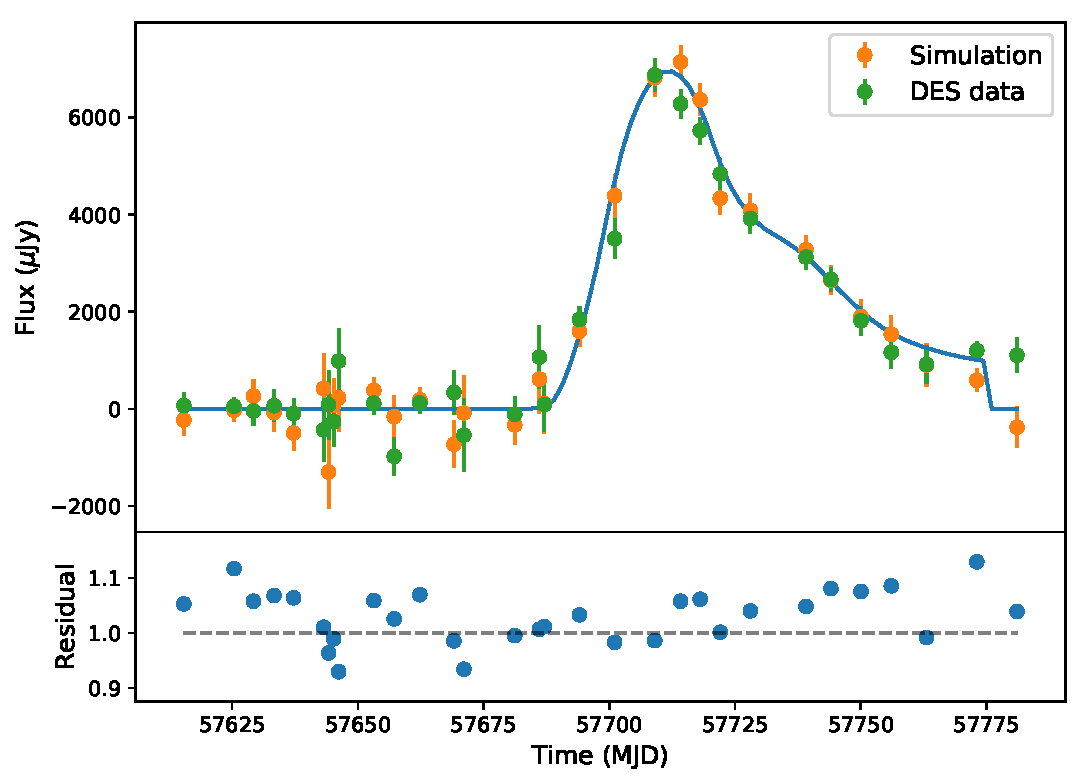
\includegraphics[width=\textwidth]{Figures/Chapter5/IaSim.pdf}
  \caption{\textit{Top}: \textit{r}-band light curve of an example SN\,Ia observed by DES and a simulated object created to replicate the original data point. \textit{Bottom}: the ratio of the S/N for the observed and simulated data light curves shown to be in agreement.}
  \label{fig:IaNoiseComp}
\end{figure}

\subsection{SN\,Ia}
Amongst the various SN classes simulated as part of this thesis, SN\,Ia is unquestionably the most well-studied and understood class of objects. Thanks to over two decades of use as cosmological probes, there exists a number of packages able to model and simulate these objects with a high accuracy. Furthermore, the parameter spaces of SN\,Ia as well as peculiar outliers to the class (SN\,Ia-91bg and SN\,Ia-91T) are well understood, giving us a firm base on which we can build their simulated samples.

While there are no limiting factors preventing us from performing our own simulations, starting with any implementation of the SALT2 model (e.g SNANA, SNCosmo or otherwise), and passing these through the DES noise model (\sref{sec:NoiseModel}), this would, in essence, replicate the sample of fake SN\,Ia injected into the science images as part of the real-time data reduction pipeline. In DES, these objects are used to estimate the image quality and generate the \textsc{SIMLIB} files making them equivalent to light curve that would be generated through SNANA.

The light curves of SN\,Ia that are injected into the images are generated using the extended SALT2 model as used in \citet{Betoule2014}. The upper redshift range was set as z=1.4 ensuring that the sample is not limited by the simulated redshift. We expect that DES is able to detect SN\,Ia up to redshift z$\sim$1.3. The fake SNe are injected such as to match the rate evolution measured by \citet{Perrett2012}. As a downside of using a predetermined sample of simulated objects, we do not have any control over the number of objects entering it. However, 45,000 objects passing the detection criteria form a sufficiently large sample of SN\,Ia. \fref{fig:IaDist} shows the redshift distribution for our training set.

\begin{figure}
  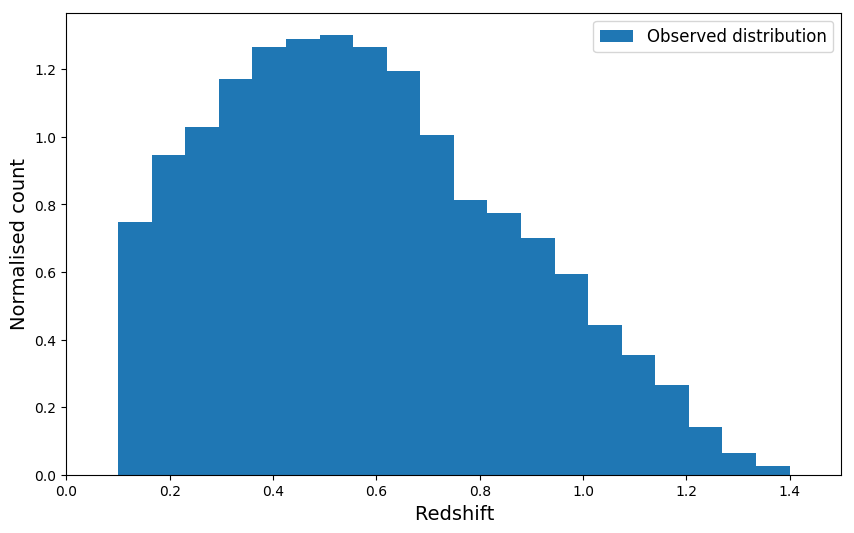
\includegraphics[width=\textwidth]{Figures/Chapter5/SNIa_z_dist.png}
  \caption{The redshift distribution of SN\,Ia that form part of our training sample. }
  \label{fig:IaDist}
\end{figure}

\subsection{CCSN}
The rate of CCSNe in the local universe is increasingly higher than the rate of SN\,Ia in the local universe, with an approximate fraction of 70\% CCSNe to 30\% SN\,Ia  \citep{Alsabti2017}. However, CCSN are a fainter with an average brightness only a tenth of the SN\,Ia luminosity that results in the survey such as DES being able to only detect them up to the z$\sim$0.6 as compared to z$\sim$1.3 for SN\,Ia, giving a much lower observed rate. In this study, it was necessary for our sample not to duplicate this observed rate as the training of CNNs requires that each distinct classes of objects entering the classification model must be equally represented.

While there is a great diversity amongst CCSNe, in terms of both their morphology and peak luminosity, our simulation package; \textsc{CoCo} (\sref{sec:CoCo}), was designed with sufficient flexibility to allow for simulating of their entire population. As the overarching aim of this thesis is the classification of SLSNe, as opposed to providing an accurate photometric classification for all transients detected by DES, a thorough treatment of the CCSNe could be considered excessive. As both SN\,Ia and SN\,Ib/c are a result of the decay of Ni56 their resulting light curves are often difficult to separate. This could essentially introduce two classes of objects which are too close in their morphology and lead to overfitting when classifying SN\,Ia and CCSNe against other species of transient objects. However, in order to avoid the introduction of any biases into our training sample, we must treat these classes as separate. Furthermore, the low redshift behaviour of the SNe, that is familiar to us, may not necessarily be reflected in the appearance of the object at higher redshifts.

\subsubsection{SN\,Ib/c}
In \cref{Chapter4}, I presented a method for creating templates as well as simulating SN\,Ib/c. I used \textsc{CoCo}, a bespoke package for the purpose of simulating over 100,000 of these objects based on the spectroscopic templates shown in \tref{tab:IbcTemplates}. Due to the low number statistics of the sample, the spectral subtypes of the templates do not match their measured relative abundance. Following Firth et al. (in prep), I use the \citet{Li2011} measurement of the local rates of CCSNe to correct their abundances. A question was raised as to whether the subclasses should be represented equally throughout the sample or match their observed rates. The decision to follow their observed abundances is based on our lack of interest in subclassifying transients based on their similarity to a specific SN template.

\begin{table}
  \caption{Sample of SN\,Ib/c used within \textsc{CoCo} as template for their class. The variation in the peak luminosity of the SNe results in different upper redshift limit at which the objects are detectable by DES. The SNe with slower evolution and greater luminosity are detected more often in the survey resulting in a higher number of accepted samples.}
  \label{tab:IbcTemplates}
  \centering
  \begin{tabular}{l|r|r}
    SN Name  & redshift & count \\
    \hline
    SN1993J  & 0.79 &  3322  \\
    SN1994I  & 0.70 &   975  \\
    SN1996cb & 0.78 &  2151  \\
    SN1998bw & 0.80 & 16416  \\
    SN2002ap & 0.80 &  2938  \\
    SN2005bf & 0.80 &  8259  \\
    SN2005hg & 0.80 &  1942  \\
    SN2006aj & 0.80 & 11988  \\
    SN2007Y  & 0.57 &   428  \\
    SN2007gr & 0.67 &   954  \\
    SN2007uy & 0.64 &   905  \\
    SN2008D  & 0.28 &   196  \\
    SN2008ax & 0.43 &   766  \\
    SN2008bo & 0.46 &   390  \\
    SN2009iz & 0.80 &  1553  \\
    SN2009jf & 0.80 &  4044  \\
    SN2010al & 0.80 & 14784  \\
    SN2011bm & 0.80 & 24213  \\
    SN2011dh & 0.73 &  2659  \\
    SN2011ei & 0.39 &   410  \\
    SN2012ap & 0.54 &   707
  \end{tabular}
\end{table}

I generate the light curves in the redshift range of 0$<$z$<$0.8, drown using a volume-weighted, non-uniform random distribution based on the star formation rate of the universe \citep{Hopkins2006}. To introduce a level of diversity into the sample, I apply host galaxy reddening to the templates (Milky Way extinction is not necessary as DES observed is very low extinction fields). I use the \citet{Cardelli1989} law with R$_\mathrm{v}$=3.7 and the A(B-V) values drawn randomly from the modulus of a Normal distribution centred at zero with a variance, $\mu$=0.2. Furthermore, I have used a similar (but unmodulated) distribution to apply an offset for the peak magnitudes of the SNe. This is further aimed at introducing a scatter into the training sample as the low number of available templates, despite being placed at different redshifts and explosion dates, could produce repeating samples of objects that could lead to overfitting.

From the simulations, we measure the detectability of each template as the function of redshift (see \tref{IbcTemplates}) as well as the detection frequency of the whole population as a function of redshift shown in \fref{fig:IbcDist}. As expected SN\,Ib/c are detectable only up to z$\sim$0.8, a distance significantly lower than that of SN\,Ia (\fref{IaDist}).

\begin{figure}
  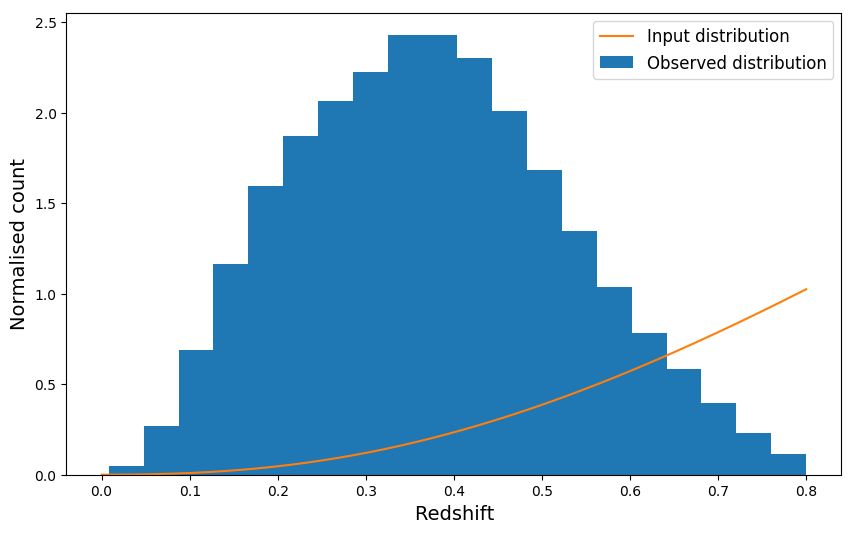
\includegraphics[width=\textwidth]{Figures/Chapter5/SNIbc_z_dist.png}
  \caption{The input distribution of artificially generated SN\,Ibc vs their detection count as a function of redshift. As expected, the detection fraction of SN rises initially with the increase in the volume of the sampled universe before declining at higher redshift due to a decrease in their detectability.}
  \label{fig:IbcDist}
\end{figure}

\subsubsection{Hydrogen-Rich SN}
The method used for building the training sample of SN\,II followed that of SN\,Ib/c very closely. I used the template sample, generated using the \textsc{CoCo} package, as present in \tref{tab:SNIITemplates}. The only significant difference in the process of generating the sample was the simulated redshift range which was increased to z$\sim$0.9 as we have found during our testing that using z<0.8 would result in a number of objects being detected at the upper redshift limit.

\begin{table}
  \caption{Sample of SN\,II used within \textsc{CoCo} as template for their class. This sample is smaller than its sister sample of SN\,Ib/c due to the lower quality of their spectroscopic data.}
  \label{tab:SNIITemplates}
  \centering
  \begin{tabular}{l|r|r}
    SN Name  & redshift & count \\
    \hline
    SN1999el & 0.40 &  4052 \\
    SN2000cb & 0.36 &  4127 \\
    SN2000eo & 0.78 & 20895 \\
    SN2002gd & 0.26 &  1924 \\
    SN2006V  & 0.45 &  7178 \\
    SN2007pk & 0.75 & 18822 \\
    SN2009E  & 0.30 &  3538 \\
    SN2010al & 0.90 & 30882 \\
    SN2011hs & 0.26 &   792 \\
    SN2012ec & 0.36 &  5176 \\
    SN2013ej & 0.36 &  4114 \\
    \hline
  \end{tabular}
\end{table}

\begin{figure}
  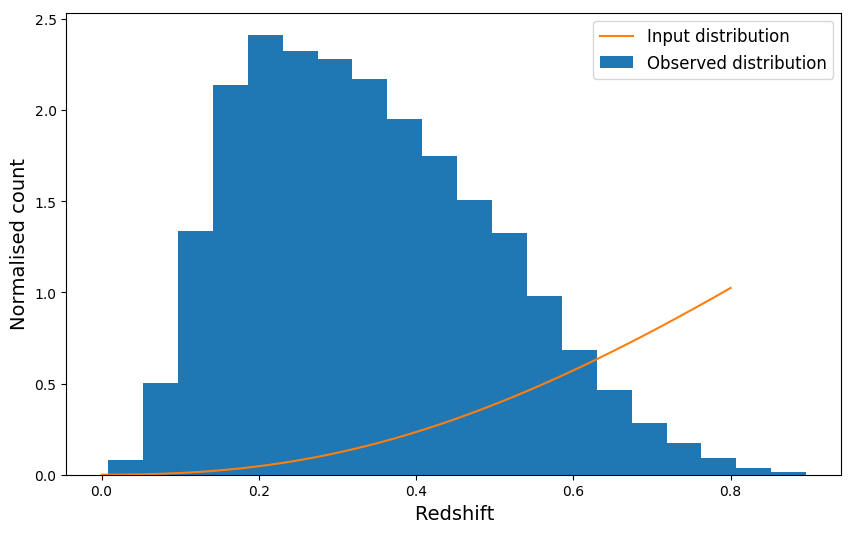
\includegraphics[width=\textwidth]{Figures/Chapter5/SNII_z_dist.png}
  \caption{The input distribution of artificially generated SN\,II vs their detection count as a function of redshift. The distribution is skewed due to the bimodality in the detectability of the training sample shown in \tref{tab:SNIITemplates} thanks to a small number of objects with a much higher intrinsic luminosity than the rest of the sample.}
  \label{fig:IIDist}
\end{figure}

\subsection{SLSN}
The simulations of SLSNe were one of the most challenging topics of this thesis. The low numbers of known examples of this class, combined with the uncertainty surrounding their definition and the engine powering their brilliant luminosity makes their modelling a challenging task. For the purpose of a classification study such as the one presented in this thesis, we must not only replicate all previously observed objects but also make a reasonable, but not overly constraining, prediction for what yet unknown SLSNe may appear as and represent as a class. Until recently, this would not have been possible as our understanding of the models of SLSNe and their parameters was not sufficient. However, several works including \cref{Chapter3,Chapter4} of this thesis as well as \citet{Inserra2013,Nicoll2013,Nicoll2017} and Angus et al. (in prep) showed that the spin-down of a Magnetar model is able to provide a good approximation for all SLSNe with an acceptable level of accuracy.

The greatest step towards simulating SLSNe was achieved in \citet{Inserra2018a} where we have established a new definition of this class that is versatile and robust enough to produce a sample that matches all observed objects but at the same time is limited in the span such that it does not overlap with other classes of SNe. This definition is based on Four Observables Parameter Space (4OPS), defined in narrow (800\AA and 1000\AA wide respectively) box filters centered at 4000\AA and 5200\AA, by: the peak in the 4000\AA band light curves, colour between the band at peak and +30 days post maximum, and the drop in magnitude between the peak and +30 days in the 4000\AA band. \citet{Inserra2018a} finds that SLSNe form linear correlations in this parameter space, with a narrow scatter shown in \fref{fig:4OPS}. I use this property to determine the magnetar model parameters which correspond to the definition of SLSNe.

\begin{figure}
  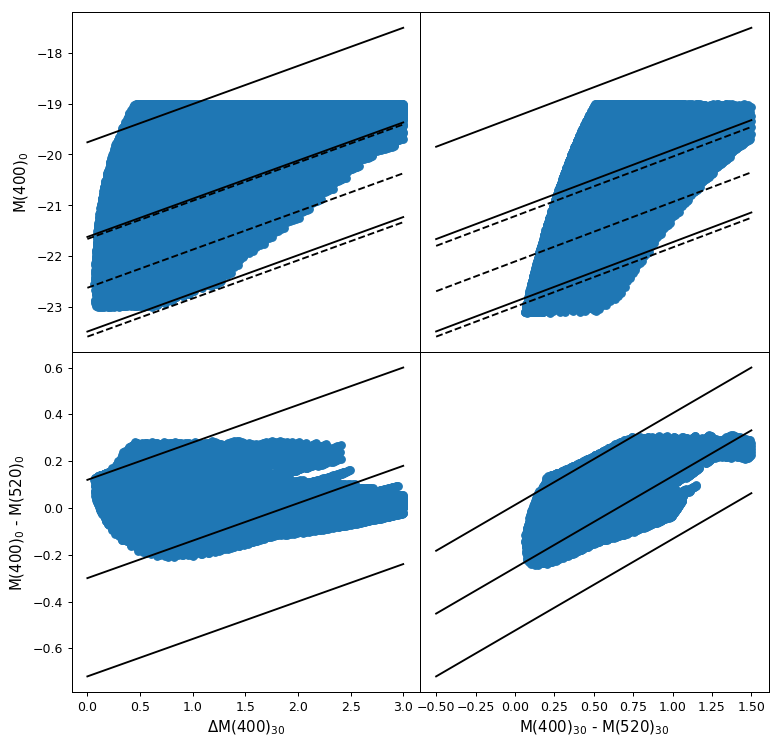
\includegraphics[width=\textwidth]{Figures/Chapter5/4ops.png}
  \caption{The 4OPS parameter space used to identify SLSNe. The solid lines represend the regions used in this work while the dashed lines are the original values found \citet{Inserra2018a}. The shaded area corresponds to the regions where SLSNe, generated using the \textsc{pyMagnetar} pipeline, that are compatible with the 4OPS definition.}
  \label{fig:4OPS}
\end{figure}

I simulate a large number of SLSNe using the magnetar model and compare them to the 4OPS definition. The magnetar model parameters are drawn randomly from a uniform top-hat distribution, bound at 10<$\tau_M$<150, 0.1<$B_{14}$<20.0, 0.01<$P_{ms}$<10.0. These limits were informed by the definition of SLSNe used in the rate calculation described in \cref{Chapter3}, but were expanded to ensure completeness and, at the same time, limit the number of computationally expensive simulations that needed to be performed. Furthermore, I introduce a modification to the 4OPS definition of SLSNe, similar to that in Angus et al. (in prep), where the parameter spaces are expanded by one magnitude of scattering while retaining the original slope of their relationship. This was aimed at including fainter objects such as those found in the DES spectroscopically confirmed sample (\sref{sec:DES_SLSN}), that were not available at the time the relationship was constructed. The modified limits are presented in \tref{tab:4OPS} and can be seen in \fref{fig:4OPS} along with the regions where objects drawn from the magnetar model.

\begin{table}
  \caption{}
  \label{tab:4OPS}

\end{table}

\begin{figure}
  % \includegraphics{/path/to/figure}
  \caption{[MAKE THIS MAG ONLY NOT 4 PANEL]}
  \label{fig:4OPSMag}
\end{figure}

In \fref{fig:4OPSMag}, I show the distribution of magnetar model parameters that produce objects that match the 4OPS definition of SLSNe. Perhaps the most interesting result is the luminosity function that results from uniformly drawing objects from the magnetar model parameter space. With no external inputs, the function matches that observed by \citet{DeCia2017} in the PTF sample of SLSNe, showing a rapid increase in the number of objects as we move towards the fainter end of their spectrum. I use the sets of magnetar model parameters that match the SLSN definition to generate their training sample. In total, $\sim$100,000 SLSN were generated at a range redshifts with 0<z<3, drawn from a volume-weighted distribution following the SFR of the universe \citep{Beacon2004} similarly to that used for simulating CCSNe (\fref{fig:SLSNDist}).

\begin{figure}
  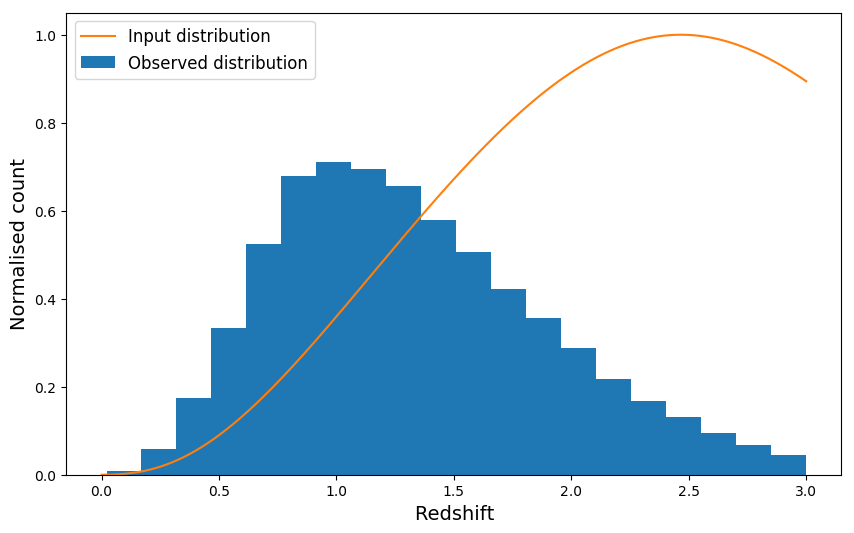
\includegraphics[width=\textwidth]{Figures/Chapter5/SLSN_z_dist.png}
  \caption{The input distribution of artificially generated SLSN vs their detection count as a function of redshift. The superior luminosity of these objects compared to other CCSNe is apparent when comparing their detectability ranges. This also motivates further our search as we know that DES should be able to detect SLSN up to z$\sim$3, while the most distant object to date was confirmed at z=2.0}
  \label{fig:SLSNDist}
\end{figure}

\subsection{AGN}
Active Galactic Nuclei (AGN) are the largest contaminant in the DES transient sample. This is partially due to their physical morphology and, in greater measure, the design of the survey. AGNs are most commonly associated with long, quasi-periodic, variable light curves that are often easy to identify based on their historical variability. As no long-term observations, matching its depth, are available for the DES SN fields making each first AGN detection its discovery. Prior to the first season of DES, a set of science verification images were taken as templates for the image subtraction pipeline used to detect new transients. AGNs that have undergone rebrightening in the first season were detected as potential supernova candidates. If the templates remained unchanged for the duration of the survey we would see a decrease in the contamination each season. Furthermore, we would be able to remove most of these transients retrospectively by selecting objects with detections in multiple seasons. The survey did, however, change the templates each year in the first three seasons of its operations to increase the quality of the images used as templates. In the final two seasons, the data from Y2 was used as templates. Additionally, the data for the first season was also later reanalysed using Y2 images as a template. A caveat of DES that caused us particular issues is that negative `detections' are not considered as detections within the transient selection algorithms. As a result, each DES season contains a large number of objects which are selected as new transients despite showing strong visual signs of prior, albeit `negative', variability.

In the cases of SLSNe, this is particularly troubling as their slow evolution can be sometimes confused with an AGN with a quasi-period of approximately one year if only single DES seasons are considered. It is, therefore, imperative that AGNs are correctly represented in the ML training sample used in \sref{sec:CNN}. For this purpose, I use the existing simulations of AGNs, in the DES observing bands, presented in \citet{Honig2016}. While these simulations were originally aimed at evaluating the possibility of using AGNs as cosmological probes, using a technique referred to as Reverberation Mapping, they were suited perfectly for this project. The simulated light curves did not include any survey noise, were densely sampled (one-day cadence) and had a span exceeding four years. In total 100,000 simulated objects were available for this study including those placed at redshifts outside the detectable range for DES. I have therefore placed each object at random start dates and fields, before applying the survey noise using the method described in \sref{sec:NoiseModel}, resulting in $\sim$60,000 detected AGNs.

\subsection{Noise}
Visual inspection of the DES light curve data shows that a limited number of objects, originally recognised as a real transient according to the DES transient selection criteria (\cref{Chapter2}), do not appear to be physical in origin. There appear to be two main origins for these objects: bad image subtractions and spurious noise detections. Despite a sophisticated, ML powered, transient selection pipeline \citep{Goldstein2015}, some objects (often elongated and with negative subtractions; \fref{fig:BadSubtractions}) can pass the ML cuts, albeit with a low score. In some cases, likely dependant on the observing conditions, this may occur in several epochs separated by less than 30 days, giving the object a `real transient' flag.

Another channel that can result in the misclassifications of candidates is the detection of slow-moving, near earth object. Such objects are most commonly detected at the same position only in two or three consecutive bands. In subsequent epochs, they are, in normal circumstances, no longer detected at the same position resulting in the object being rejected. However, in some rare cases, bad subtractions or random noise spikes exceeding the 5 sigma detection limit, within 30 days cut can result in a `real transient' flag.

\begin{figure}
  % \includegraphics{/path/to/figure}
  \caption{}
  \label{fig:BadSubtractions}
\end{figure}

To model these objects, I use a very simple approach of inserting a number of sharp, $\delta$-function like spikes in the data that correlated between the filters and separated by less than 30 days to account for the misidentifications. The spikes are selected between 19$<$mag$<$22 in order to test the different behaviours of the GP interpolations used in the next step of this analysis (\sref{sec:DataAugmentation}). The absolute value of the peak does not play an important role in the classification process as the data is normalised before entering the CNN. Similarly to other classes of transients, $\sim$100,000 objects have been simulated across all fields.

\subsection{Missing classes}
While in this thesis, I have created one of the most thorough training samples of SNe for the purpose of a ML classification study, it still cannot be said to be complete. There are a number of classes of known transient objects which I was unable to account for in this work. Some objects such as kilonovae, associated with gravitational waves as their optical counterparts, evolve too rapidly to be using the cadence of DES. Omitting these (undetectable) events does not bring any difference to the final result of our classification. However, one class of objects which could have an effect on our final classification are the newly discovered class of rapidly evolving SNe \cite{Drout2014,Kepler2018}. Recent work by \citet{Pursiainen2018} showed that these objects are relatively common within DES with 72 detections in the first four seasons of its operations. While there are now early, tentative signs \citep{Pursiainen2018} that these objects are powered by a SN shock interacting within a thick an extended wind \citep{Piro2015}, similar to the model used in modelling of the `bumps' found in SLSNe \sref{sec:MagExtensions}. It is this particular connection that would be interesting to explore, however, the modelling of these objects is still in its infancy. The model parameter spaces defining them, their SED models and other similar aspects developed for SLSNe over the last several years have not yet been studied for these fast-evolving SNe.

The omission of rapidly evolving SNe from our sample will result in these objects being mislabelled in our classifications. It would, however, be unlikely that any of the objects that we have not included in the training sample would get mislabelled as a SLSNe due to their significantly faster evolution. I test this assertion in \cref{Chapter6} using the ground-truth sample of objects identified by \citet{Pursiainen2018}.

\section{Data Augmentation} \label{sec:DataAugmentation}
Before the training sample of SNe created in \sref{sec:TrainingSample} can be used to build a CNN classification model, it has to first undergo a number of augmentation steps. The data passed through the CNN must be uniform in terms of the number of data points as well as their separation, regardless of the field and season the data originated from. To achieve this, I must first select a suitable length of observations and cadence that overlaps the most closely with that observed by DES. Furthermore, I apply a flux correction required to normalise the effect of using a varying subtraction template in a different season. Finally, I use GPR to interpolate and augment the data such as to meet the requirements of CNN.

\subsection{Choosing the observing block} \label{sec:ObsBlock}
I define the observing block, for the use in our classification study, as the span of time (measured in days) that is the longest period over which all DES season observes all of its fields. Due to the observing conditions and scheduling, the DES observing periods vary between the seasons and fields. The difference between the longest and shortest observing window in DES measures 40 days.

Selecting the observing block is more complex than simply selecting the length of the shortest season. \fref{fig:ObsBlock1,fig:ObsBlock2,fig:ObsBlock3,fig:ObsBlock4} show the cadence of DES in Y1-4 in all fields and bands. Instead, this is done in two stages: first I find the span that covers all the filters. From the first point where all the filters are observed to the last point where all the filters are observed. I then remove the points at the beginning of the season in cases where the gap in the data is longer than 10 days. This is a common consequence of observation being missed due to the atmospheric conditions. Data does not have to be similarly removed at later stages of the light curve as the GPR interpolation can account for large gaps as long as they are supported by a number of points either side of the intermission.

From these measurements, I determine the optimal observing block to be 149 days in duration. The span covered by the block in each season and filter is shown in \fref{fig:ObsBlock1,fig:ObsBlock2,fig:ObsBlock3,fig:ObsBlock4}. Due to the improved quality of the light curves in the second part of each season, I place the observing block as late in time as possible.

\begin{figure}[h]
  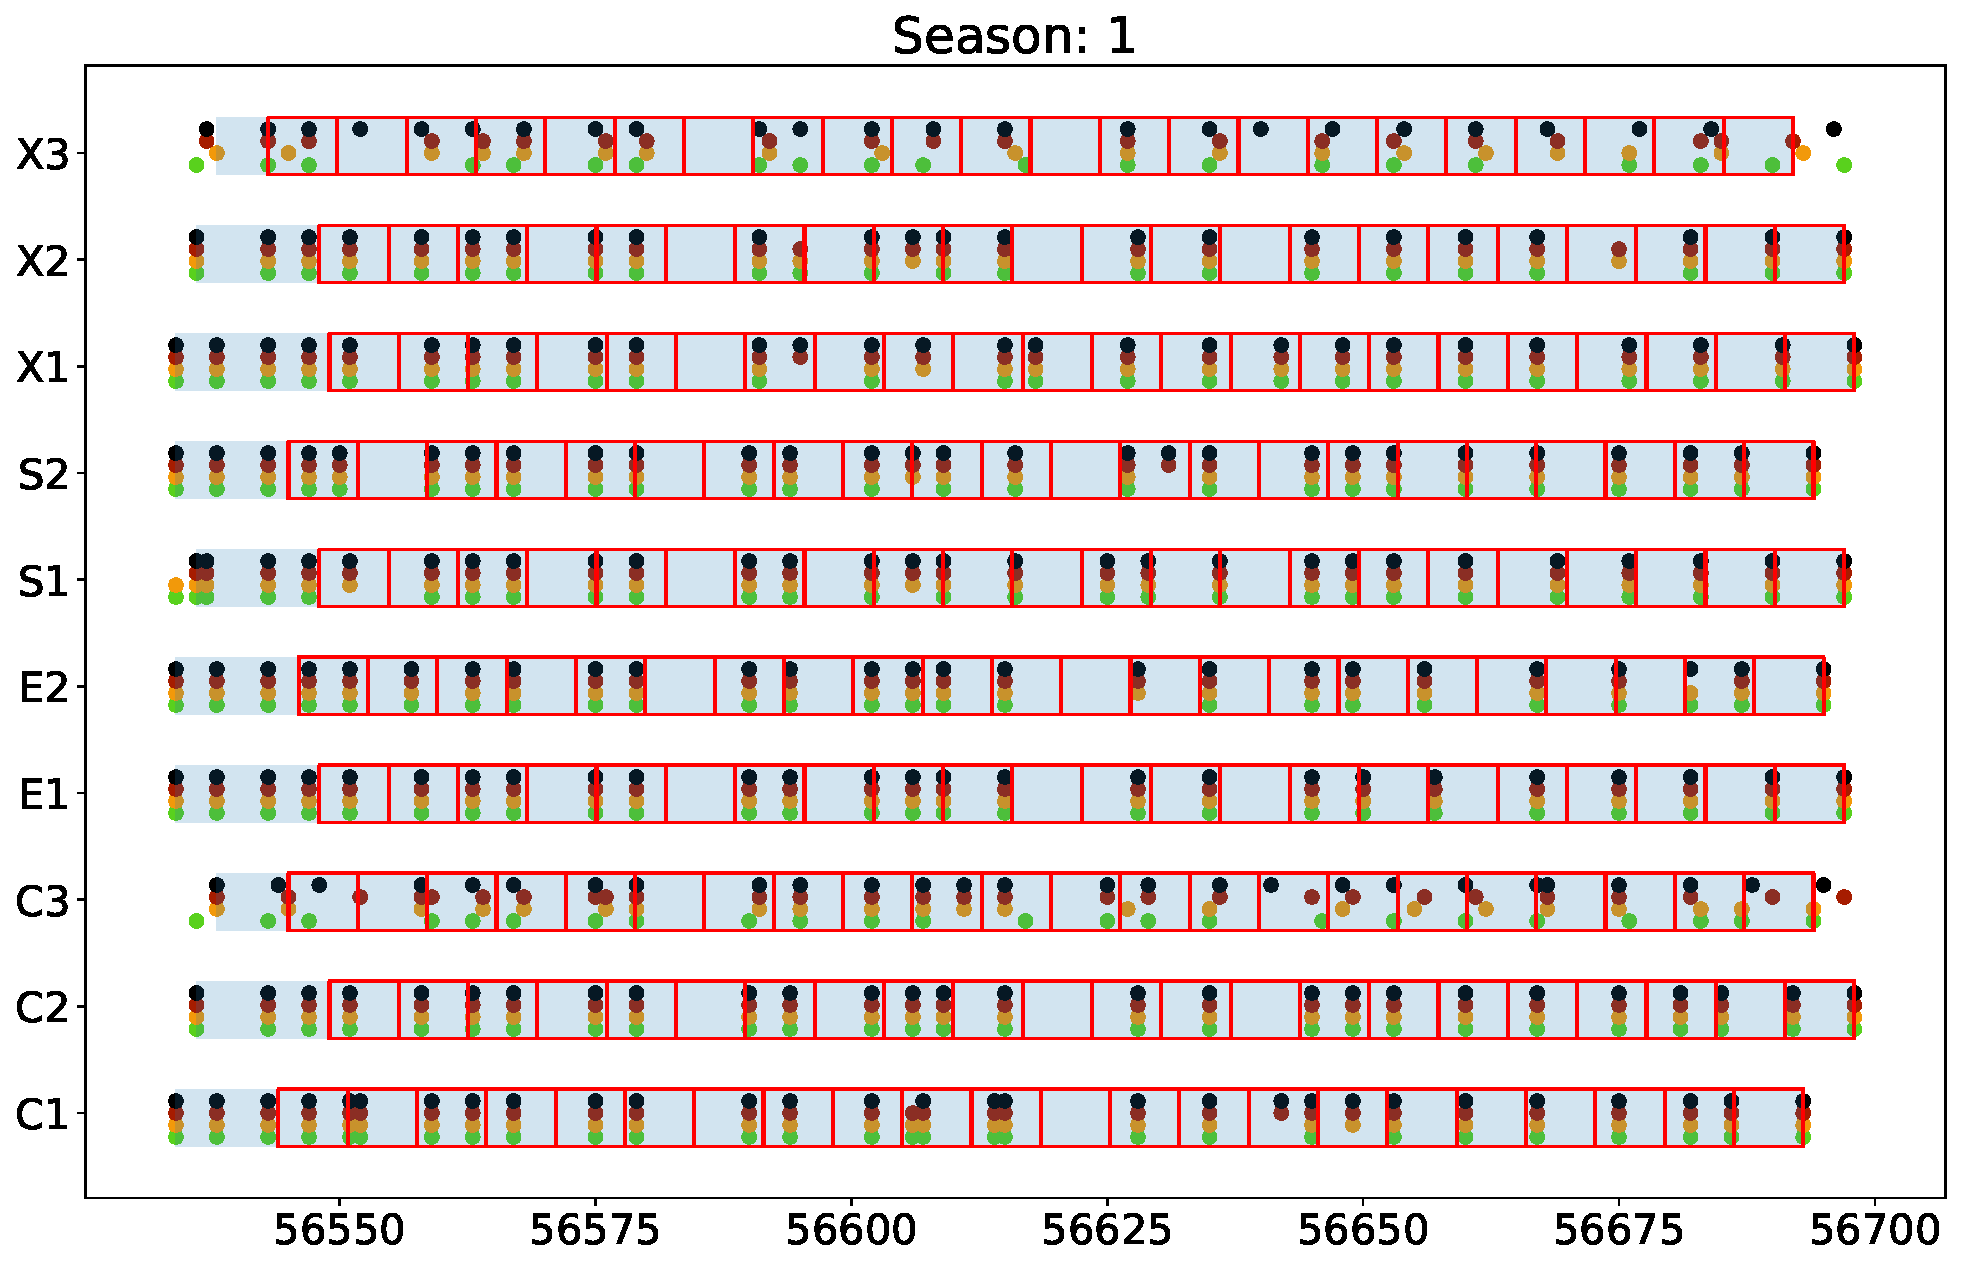
\includegraphics[width=\textwidth]{Figures/Chapter5/ObsBlock_Season1.pdf}
  \caption{The cadance and observing block of the first season of DES}
  \label{fig:ObsBlock1}
\end{figure}

\begin{figure}[h]
  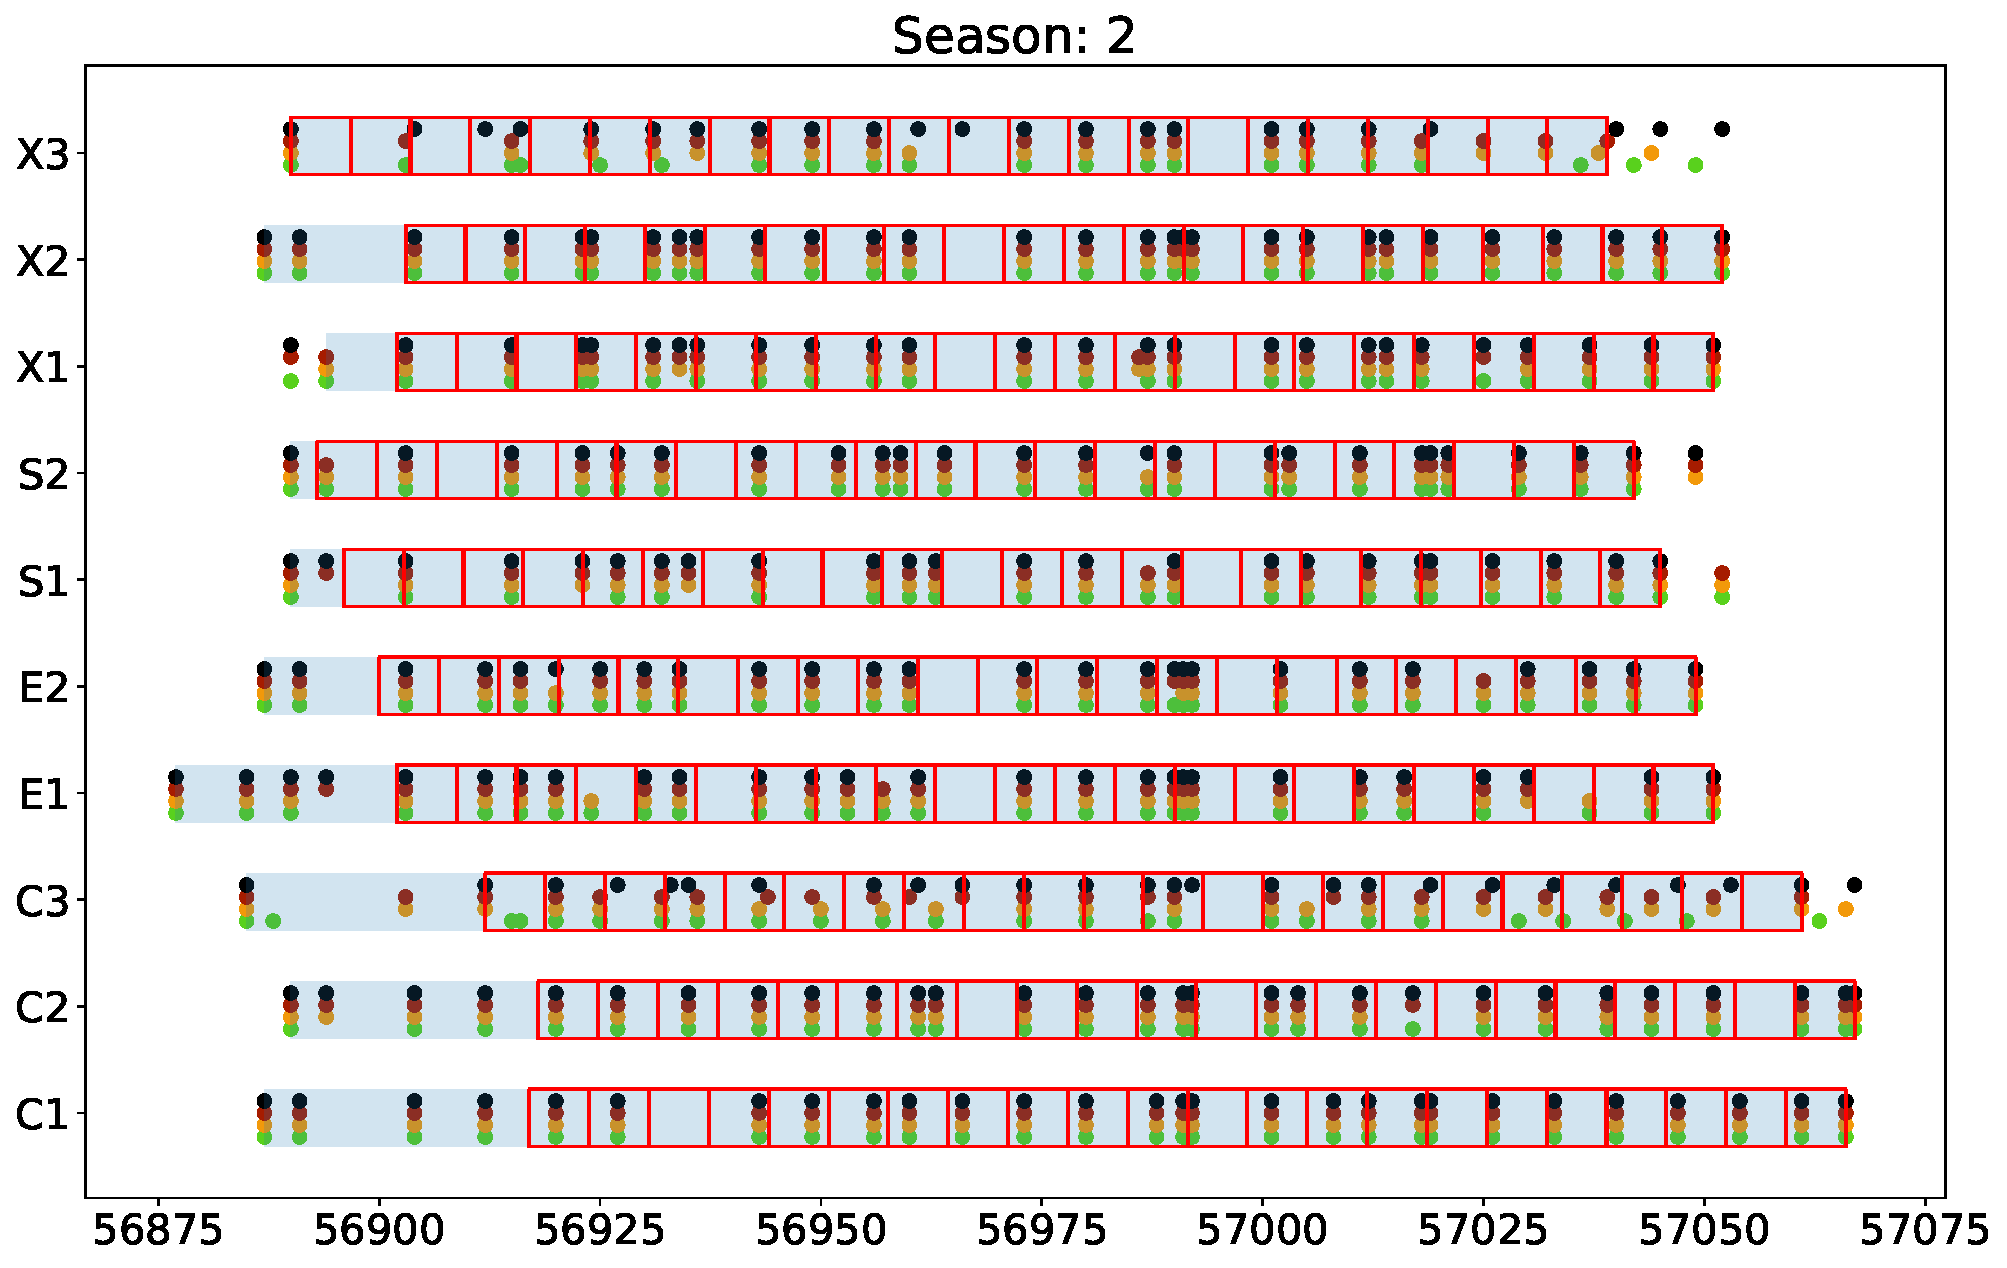
\includegraphics[width=\textwidth]{Figures/Chapter5/ObsBlock_Season2.pdf}
  \caption{The cadance and observing block of the secon season of DES}
  \label{fig:ObsBlock2}
\end{figure}

\begin{figure}[h]
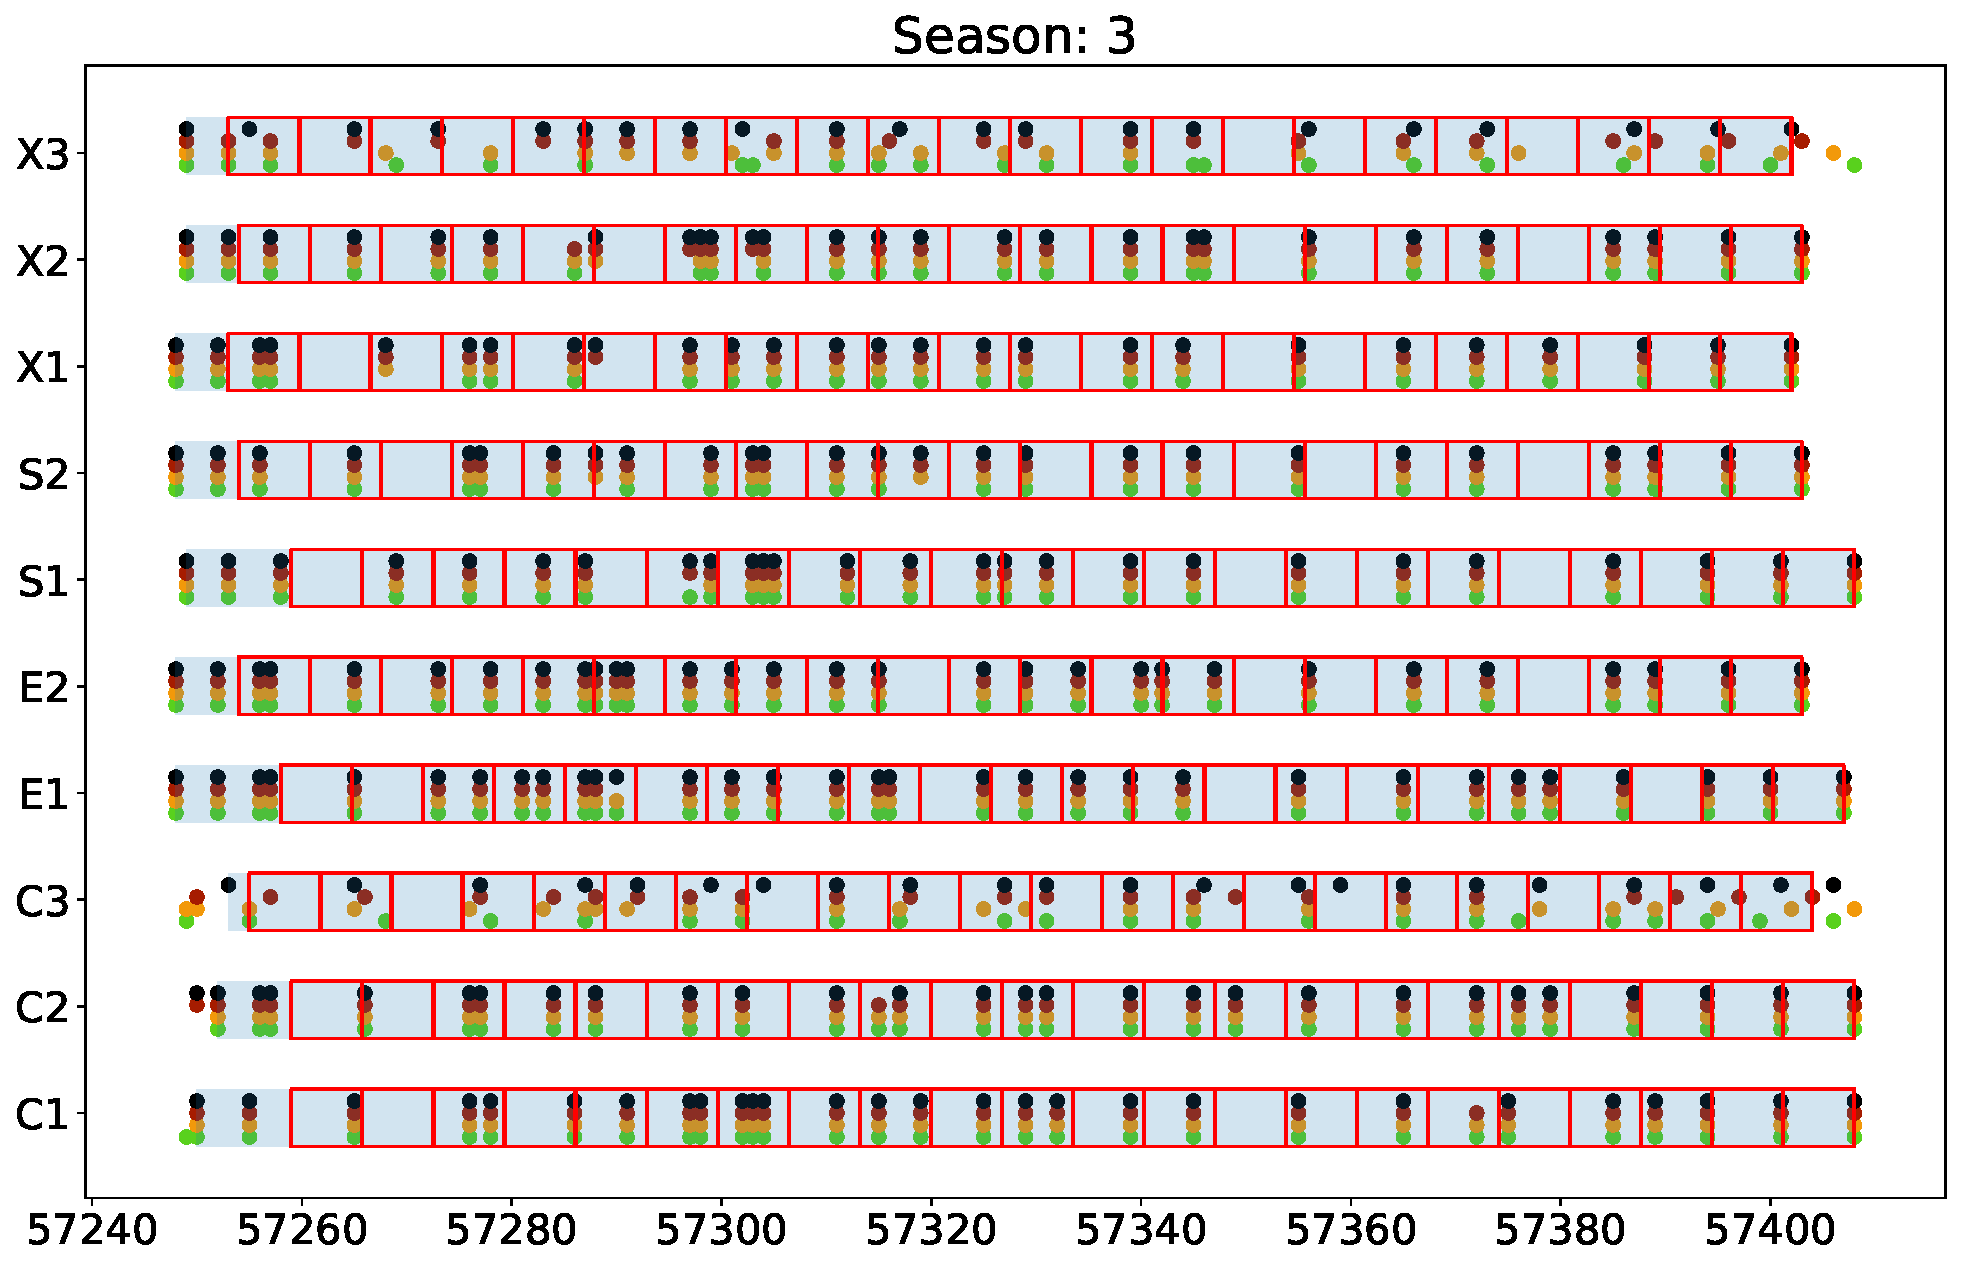
\includegraphics[width=\textwidth]{Figures/Chapter5/ObsBlock_Season3.pdf}
  \caption{The cadance and observing block of the third season of DES}
  \label{fig:ObsBlock3}
\end{figure}

\begin{figure}[h]
  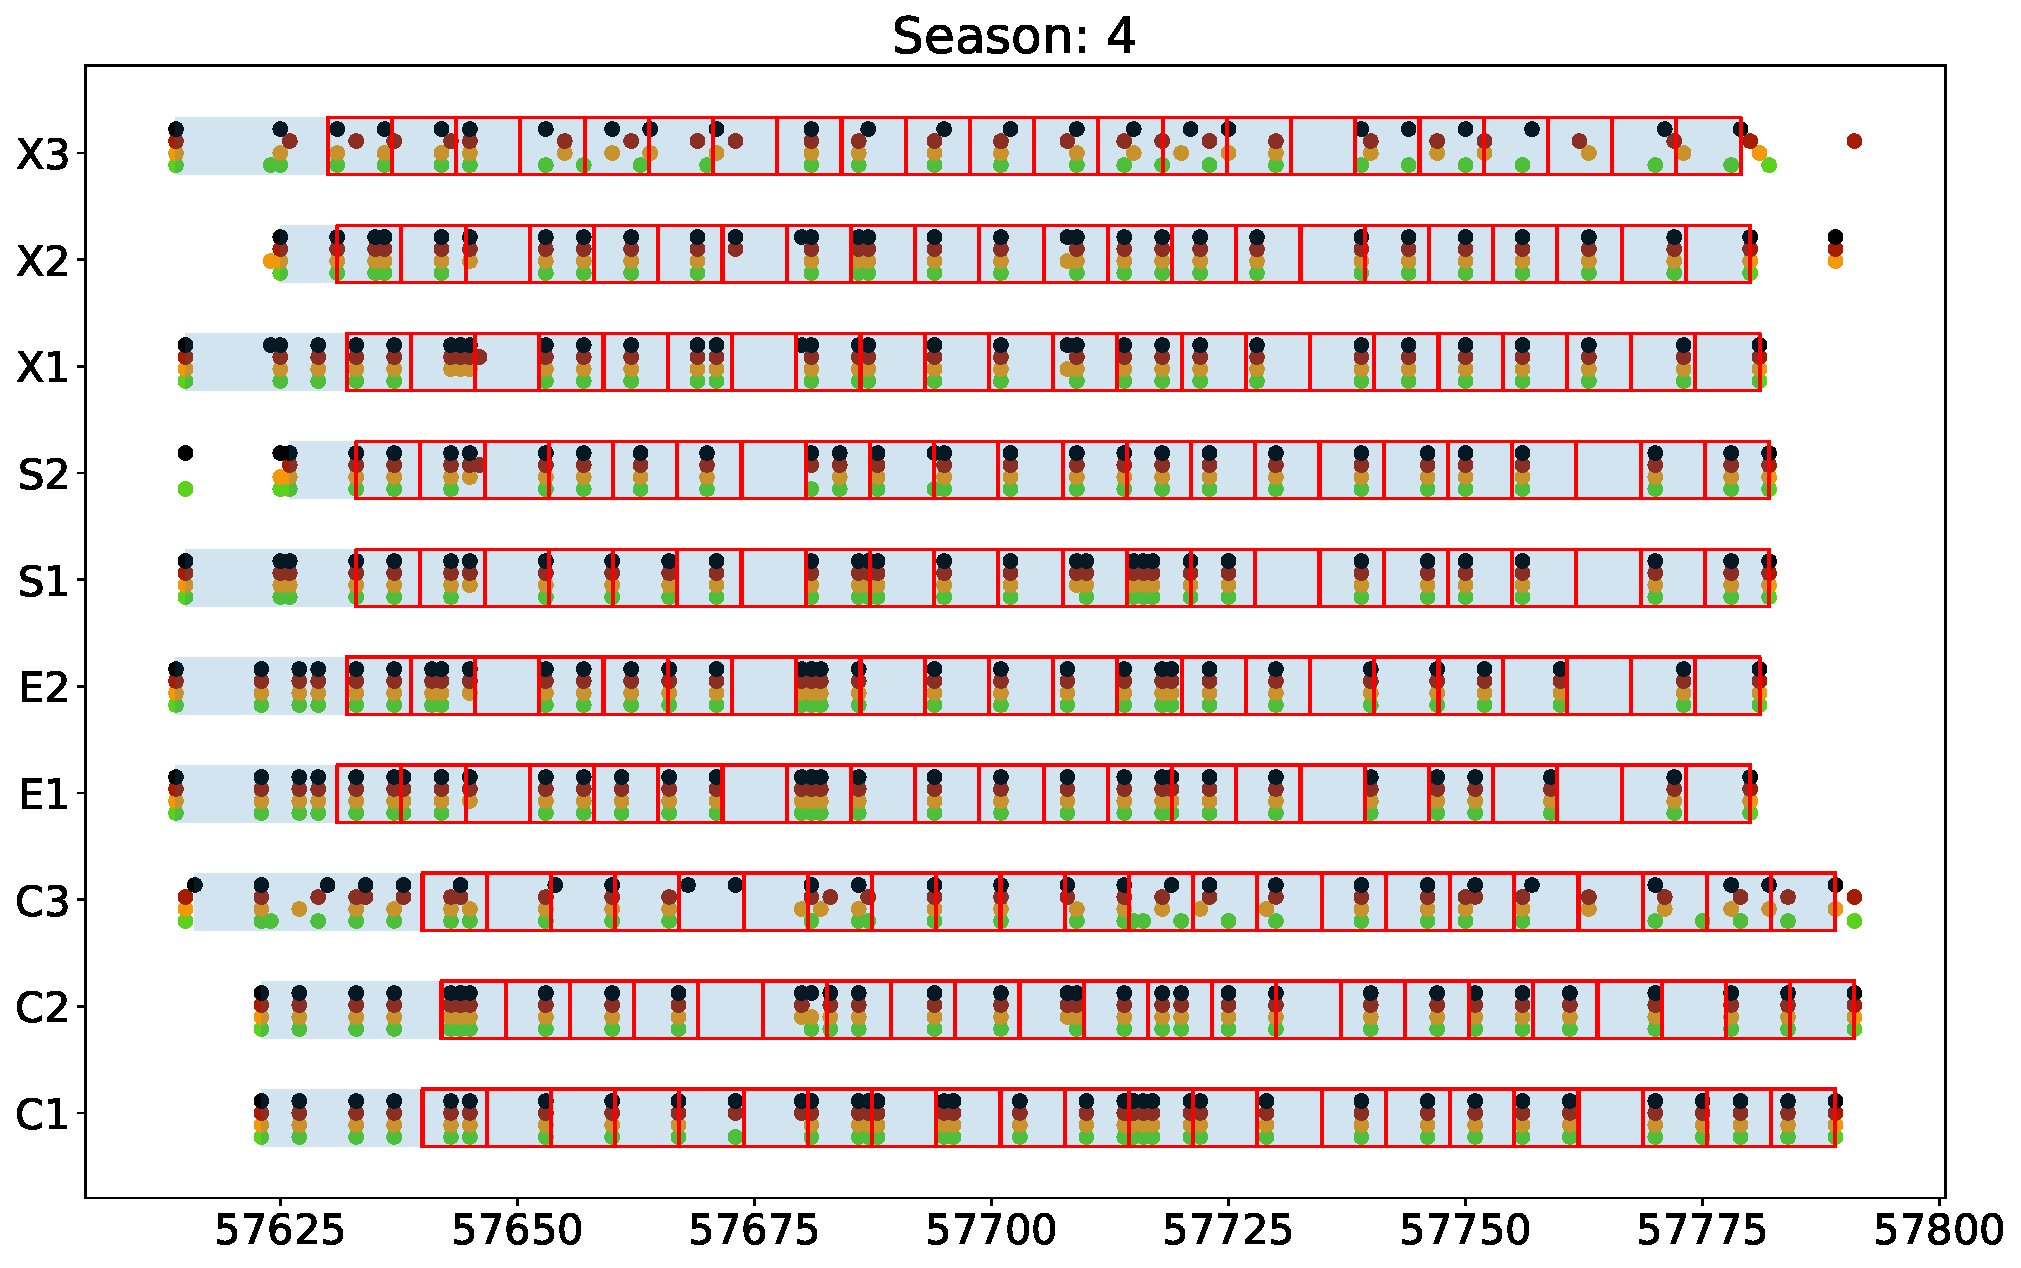
\includegraphics[width=\textwidth]{Figures/Chapter5/ObsBlock_Season4.pdf}
  \caption{The cadance and observing block of the forth season of DES}
  \label{fig:ObsBlock4}
\end{figure}

\subsection{Choosing the cadence} \label{sec:SimCadance}
Upon deciding the length of the observing block used in the simulations, the next step is to choose the cadence of the interpolated observations. As GPRs are used to augment the data, essentially any cadence can be used. As there are no rules or precedences set out in the literature that discuss the optimum treatment of the augmented data, I must make an informed decision based on all the available information to me. The factors which balance our decision is on one side to represent the data without the loss of any information observed by the survey, while at the same time not introducing too many points which, essentially, duplicate the information.

The observed cadence of DES is not uniform and varies through the season due to the observing conditions. Early in the season, the cadence is shorter as the observing weather conditions don't allow for the observations of the wide DES fields leading to a shorter DES cadence as the deep and shallow fields are given more observing time. On the opposing end, the cadence stabilised as the season progresses and settles at the designed 7 days. This is seen in \fref{fig:cadence} resulting in a bimodal distribution with an average cadence of 5 days. With a lack of any other factors, I use this value as the base for the cadence used in \sref{sec:UseGP}.

\begin{figure}
  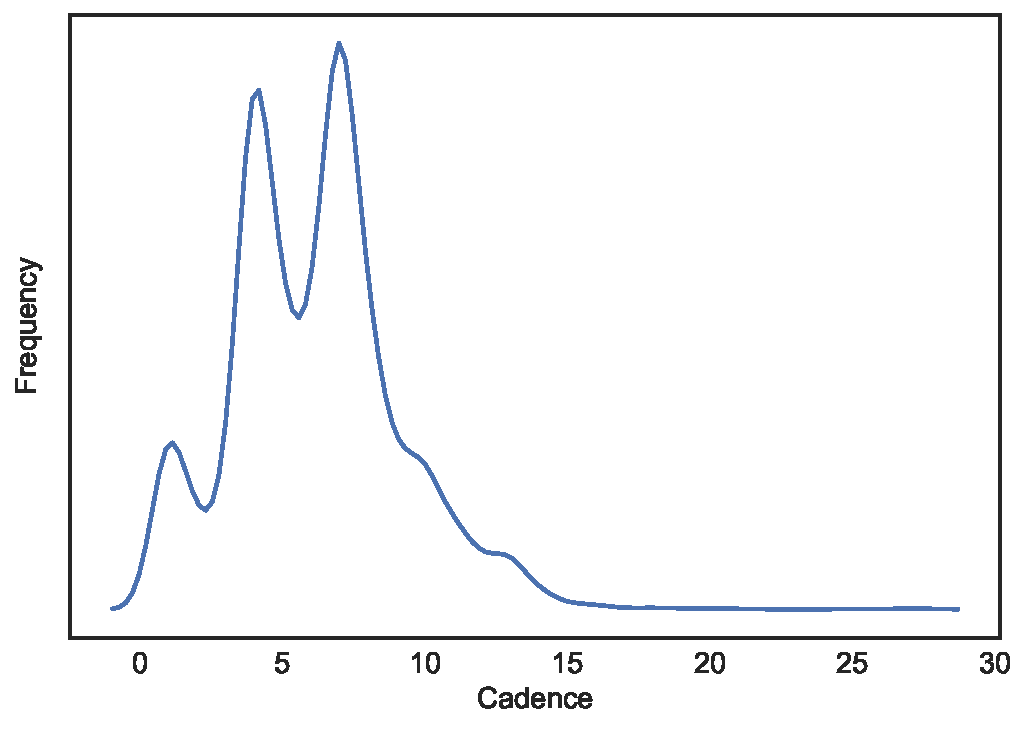
\includegraphics[width=\textwidth]{Figures/Chapter5/Cadence.pdf}
  \caption{Kernel Density Estimate (KDE) plot showing the cadence of DES across all seasons, field and bands. The bi-modality of the distribution can be attributed to the balance between the designed DES cadence of 7 days, occurring only in the perfect conditions, and the actual cadence of 3 days observed in the early parts of each season.}
  \label{fig:cadence}
\end{figure}

\subsection{Applying Flux correction to Real Data}
Before the GPR can be applied to the data, it must first be corrected for the effects of DES exchanging the image subtraction template between seasons. As the focus of the DES SN team is predominantly the study of SN\,Ia, the decision was made to maximise the quality of single-season light curves. As the image quality improved throughout the initial two seasons of observations the, templates have been updated each year. While optimal for the study of short transients, where only a single season is of interest, for slowly evolving SNe (and AGNs) this causes an issue where the supernova light curve is present in the template resulting in decreased flux in the subsequent season. This is a particular problem for SLSN, where their evolution can often be slow enough to be detectable in multiple seasons in DES (Angus et al.; in prep). This could potentially be a strong factor leading to the misclassification of SLSNe and hence cannot be ignored.

While the most optimal approach to this would be to perform the image subtraction and source detection with a single template, this would be computationally prohibitive due to the scale and complexity of the raw DES data. As an alternative solution, I used the DES analysis logs to determine the observations have been used in the creation of the template images. In these frames, I measure the median flux of the object and use this value to correct the offset. As a simple test for this approach, I use a light curve of a SN\,Ia that exploded early in the second season of DES. In the uncorrected DES light curves, this results in a flat but negative light curve in the third season. \fref{fig:FluxOffset} shows the original and corrected light curve, consistent with zero flux in the third season.

\begin{figure}
  % \includegraphics{/path/to/figure}
  \caption{}
  \label{fig:FluxOffset}
\end{figure}

\subsection{Applying GPs} \label{sec:UseGP}
The size and extent of the training sample used in this thesis are one of the two advancements made towards classifying SNe in DES using the ML approach. An equally important step, crucial for the use of CNNs, was the use of GPR (\sref{sec:GP}) as a tool for light curve interpolation and augmentation. CNN performs pattern recognition using a set of convolutional kernels with a fixed size, therefore requiring the data to be evenly sampled. This has tremendous benefits as it does not require any feature extraction steps and uses every data point in the classification process. While the observed data cannot be used directly with this technique due to its non-uniform sampling, using a GP interpolated light curves removes less information about the data than a parametric model. Simultaneously, it does not introduce any correlations between the distinct bands, both in terms of the flux and the onset of the SN.

I apply the method described in \sref{sec:GP} to interpolate the light curves using the Mate\'rn 3/2 covariance functions. I perform the interpolation over the period selected in \sref{sec:ObsBlock} using the base cadence found in \sref{sec:SimCadance}. After testing the CNN in \sref{sec:CNN}, I found that using a cadence which doubles the original 5 days, to 2.5 days, improves the accuracy of the model. The motivation behind the doubling of the cadence was to allow a gradient for each point to be calculated closer to the point itself as opposed to between the points. The extra points act as control points in this scenario.

While the fitting performed correct interpolations all of the artificially generated light curves, it did fail for a small amount of real DES objects. I reviewed these visually and determined that this is caused by errors in the extraction where some data points are associated with no uncertainty.

\section{Classifications} \label{sec:CNN}
The construction of the artificial DES training sample of transients was a major step towards performing their comprehensive classification study using the ML approach. In recent years, the use of ML expanded far beyond the purely academic uses within the field of Computer Science. The world around us is currently being shaped by Artificial Intelligence (AI) augmented technologies, driven in large measure by Artificial Neural Networks (ANN) and their derivatives such as Convolutional Neural Networks (CNN) and Deep Learning.

The process of selecting transients for spectroscopic follow-up is an example, albeit not explicit, of SN photometric classification. This task has been performed manually, via the visual inspection of the light curves, for decades in every SN survey. In recent years a number of attempts have been made to devise a pipeline for photometric classification of SN based on the clustering of light curve model parameters. However, this problem can be approached from a more fundamental point of view using AI. Computer vision, a prominent branch of AI, has been successfully applied to countless examples of classification tasks where humans demonstrated a superiority over the early classification methods. Projects such as ImageNet \citep{Russakovsky2014} were able to produce models capable of identifying a number of everyday entities (humans, vehicles, animals, household items) with an accuracy exceeding that of an average human. While the scarcity of the training samples available to us in comparison to projects such as ImageNet does not allow us to use an equally complex model, this is not required as the complexity and diversity of our transient data is not as high as that of an everyday object.

In this section, I describe the use of Convolutional Neural Networks (CNN) as an AI tool used to first identify SN light curves in the DES data and subsequently classify them into their respective subclasses with the overall aim of producing a photometric sample of DES SLSNe.

\subsection{Convolutional Neural Networks} \label{sec:CNN}
CNNs are currently one of the hottest topics in the world of AI and ML. While their widespread use is novel and a result of the increase in the performance of computer devices, the theory behind them dates back to the early work on Artificial Neural Networks \citep[ANN;][]{Mcculloch1943} and replicating the ability of the human ability to learn based the external stimuli.

\subsubsection{Artificial Neural Networks}
All principal components of an ANN are fundamentally based on the human brain contain neurons, represented by nodes and activation functions. The nodes, usually arranged in a network of layers, are connected by a set of weight that corresponds to the biological synapsis. The aim of an ANN is to perform a non-linear transformation between the input parameters and the output values.

ANN is formed through a network of fully interconnected layers, containing activations functions that, in essence, calculates the weighted sum of the inputs and creates an output that acts as an input for the next layer. The choice of activation functions is extremely important to the performance of an ANN. The most commonly used form; the sigmoid function produces an output near to one for inputs that are accepted and zero for the rejected values. The Rectified Linear Unit (ReLU), another commonly used activation function, acts in a similar way but produces a linear output that tends towards infinity above a certain activation value.

The choice of the number of layers is dictated by the complexity of the problem tackled by the network. Between the input and output layers lays a number of hidden layers. While the input later must match in size the dimensions of the input dataset and the dimensions of the output later must match the number of individual classes present in the training set, the hidden layers can have an arbitrary shape. The process through which the networks calculate the weights is referred to as Backpropagation which performs a form of a stochastic gradient descent to optimise the loss (or residual) function. There is numerous implementation of the loss functions and backpropagation algorithms, however, in this work, I chose to use the defaults found in the TensorFlow package: `cross-entropy' and `Adam' respectively.

\subsubsection{Convolutional Neural Networks}
Convolutional Neural Networks (CNN) is a type of Deep ANNs where at least one layer is a convolutional layer. These layers are designed to work similarly to edge and shape enhancing features found in popular image processing software, but instead of relying on predetermined forms learn to best match the structure of the objects found in the training sample. An important feature of CNNs is additional Pooling layers which extract the enhance information from the convolved data through a process of dimensionality reduction. The most commonly used Max Pooling layer works by passing a sliding window, of length $n$, over the data convolved with the filters, with length $m$, and selecting the highest valued pixel to create new output data with length $n-m+1$

\subsection{SNe vs AGN vs Noise}
While CNNs are extremely powerful in their ability to classify images, regardless of what they contain, they often rely on huge amounts of training samples in order to learn their discriminating features. In the case of DES transient data, we are still not operating on a sufficiently large dataset despite the work on enhancing the sample. However, it is possible to simplify the classification problem to reduce the number of training samples required to produce a good classification score.

\subsubsection{Choosing the training sample} \label{sec:AGNNoiseSNSample}
As the first step in the analysis of the DES sample, I separate the task of classifying SN from that of identifying real SN transients amongst the background of spurious detections and AGNs also detected by the survey. As the training sample for each class must be of similar shapes, I use all of the $\sim60000$ fake AGN generated in \sref{sec:AGN} as well as a random sample of 60,000 spurious noise examples. The matching SN sample must contain examples of all SN in approximately equal proportions. I therefore use 20,000 SN\,Ia, 10,000 SN\,Ibc, 10,000 SN\,II and 20,000 SLSN all drawn randomly from their respective simulated samples (\sref{sec:Augmentation}).

\subsubsection{Reshaping the data}
Due to their complexity, CNNs rely heavily on fine-tuned optimisers for minimising the model's loss functions. As a result, the data must satisfy a number of strict criteria in order to comply with these constraints. While most of them, such the need for the data to be linear, are naturally satisfied by the training dataset, we must observe a number of the constraints, including the upper and lower limits on the flux which must be in the range of positive and negative unity.

As the final piece of book-keeping, the data for all training samples must be concatenated into a single, multi-dimensional matrix, shaped such as to separate the features which are dimensionally independent of each order. In order to allow for the models described in the following section to extract both the colour and morphological evolution of the transients, each season of data is represented by a 4$\times$46, two-dimensional vectors, corresponding to the number of photometric bands and epoch per band respectively. This central block of data is built for each season independently, as the large gap between the observing blocks means that the data cannot be treated as continuous.

\subsubsection{Designing the network} \label{sec:AGNNoiseModel}
The design of a neural network is driven through a process of trials and errors as no clear formalisms available as a guideline for the process. While some early work is being  undertaken at Google in the area of automating the design of the networks for maximum performance, this is a very computationally expensive task and therefore prohibitive for us. In the case of this thesis, I am instead relying on my domain knowledge of the distinguishable features of transients to optimise the performance of the learning process.

The CNNs presented in this chapter underwent many iterations with a wide spread of layers complexity. In all instances, the first point of access in the model is a convolutional layer containing 30-80 independent filters each between 3-9 epochs wide. These filters are applied to every season and band independently. A max pooling layer is applied to the data at this point as a way of emphasising the features highlighted by the convolutional filters before a second convolutional layer, orthogonal to the first layer, is applied to the data in order to measure the colour at each epoch. At this stage, an average pooling layer is used again extracting the two most prominent features in the colour space for each filter.

After comparing a large number of iterations of these hyperparameters, I found that using 50 filters spanning 5 epochs in the first layer and 30 filters in the second layer produced the highest accuracy model. Perhaps counterintuitively, iterations, where I combined these filters together into a single two-dimensional filter, did not provide higher accuracy. A low number of orthogonal filters provides a freedom for the features to be learned independently, and prevent them from relearning the same features. One could imagine a situation where a similar light curve shape may be associated with a different colour evolution for a different class of transients. This highlights the importance of allowing the CNN to build its own features out of the simplest building blocks without overcomplicating the design by constraining the model.

\begin{figure}
  \centering
  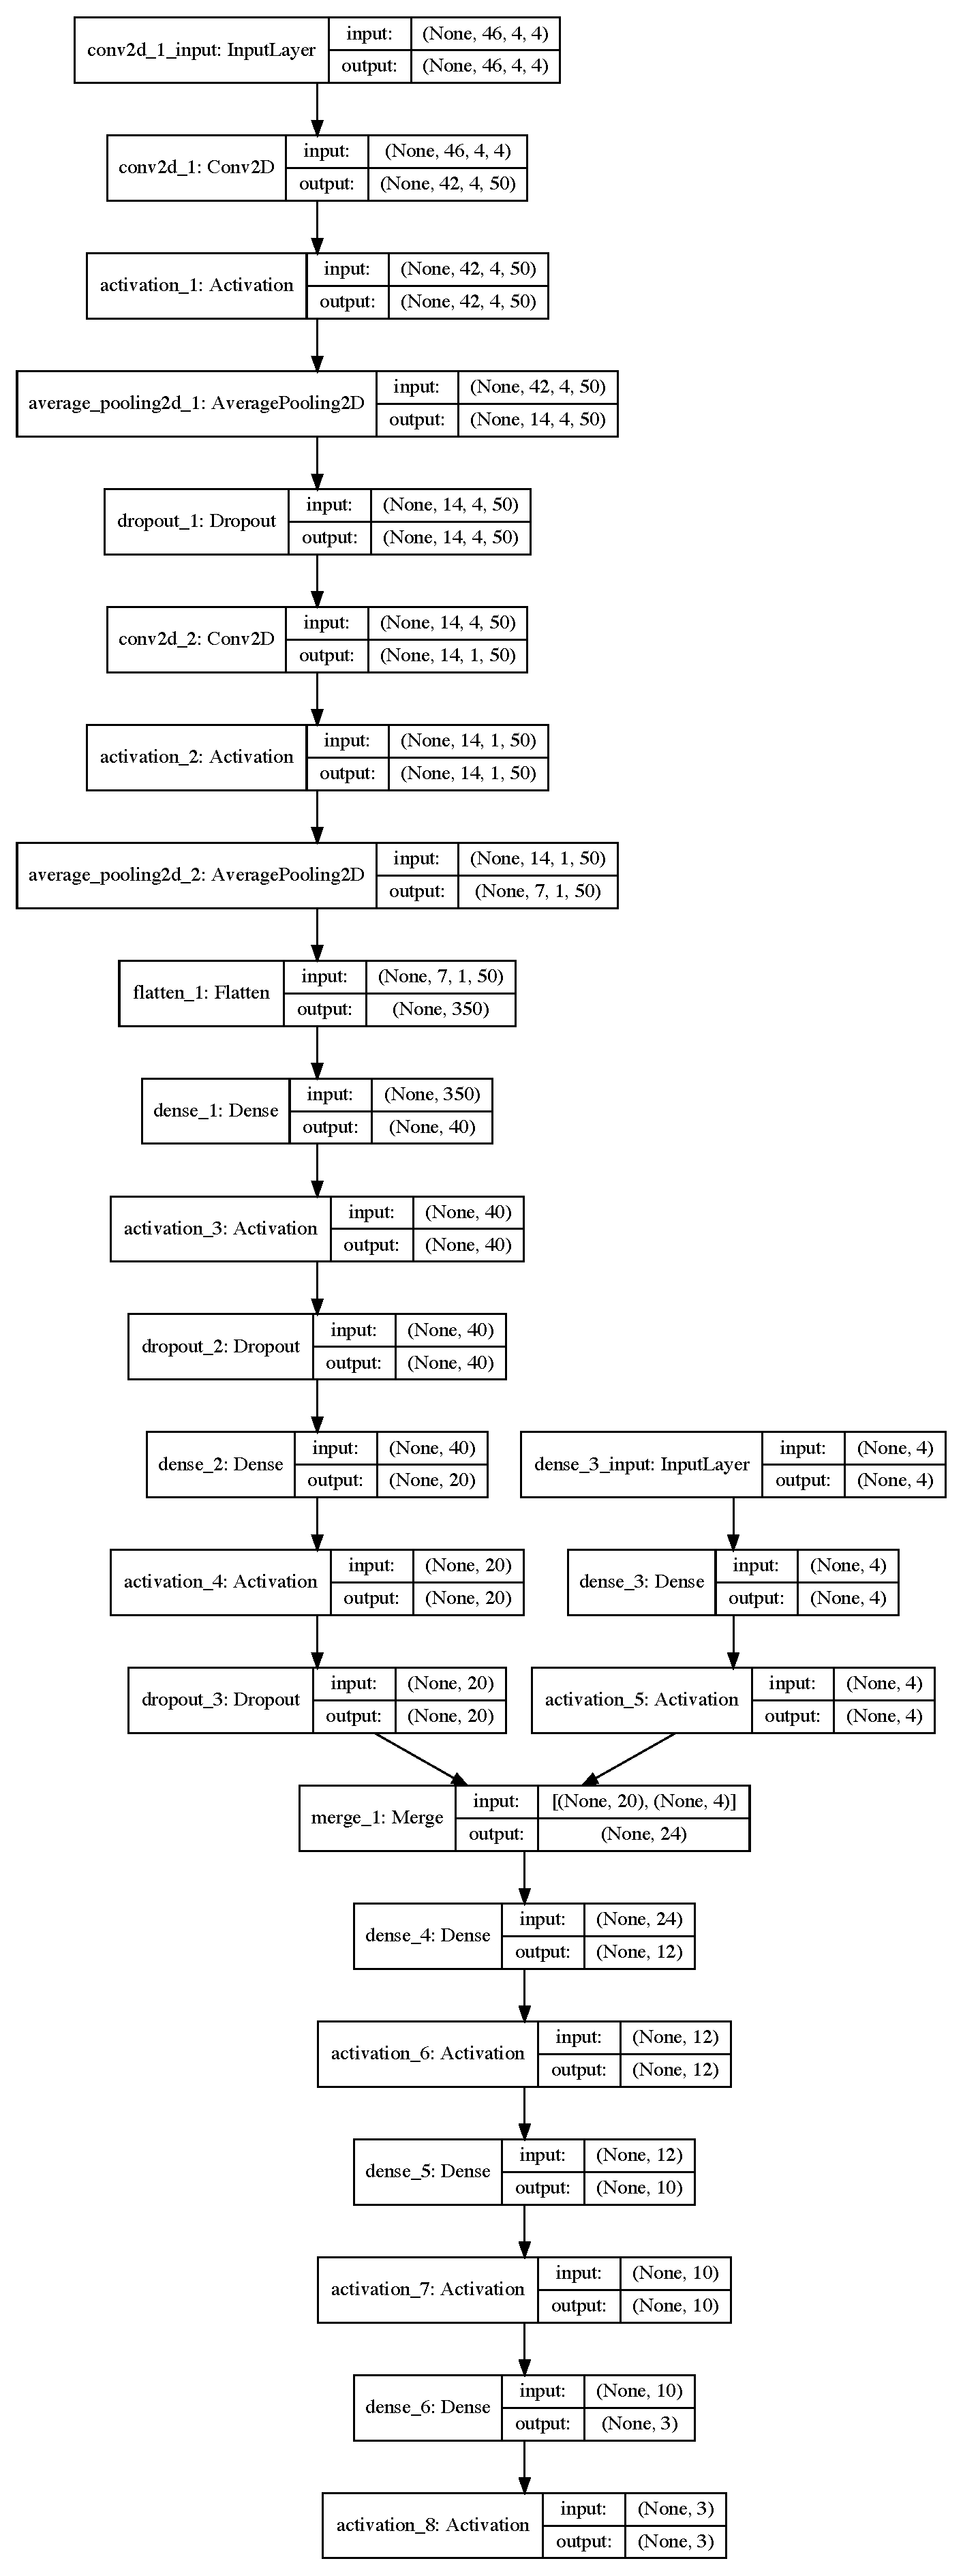
\includegraphics[width=0.6\textwidth]{Figures/Chapter5/SNAGNNoise}
  \caption{The CNN used for classification of SN vs AGN vs Noise. Each layer is labeled with its function within the network as well as its input and output dimentions.}
  \label{fig:AGNNoiseSNModel}
\end{figure}

\subsubsection{Training the model}
The combined training sample build in \sref{sec:AGNNoiseSNSample} is passed through the network using a batch size of 5000 objects with 100 epoch, or individual runs of the backpropagation algorithm. CNNs are often trained on smaller batches of data to accelerate the learning process and help to prevent overfitting. As a general rule of thumb for the choice of the number of the fitting epoch, the fitting is stopped when the model approaches convergence as an excessive number of epochs would allow the model to `learn' the test sample leading to overfitting.

My best model, as described in \sref{sec:AGNNoiseModel}, converges rapidly to the accuracy of 99.7\% which vastly exceeded our expectations. \fref{fig:AGNNoiseROC} shows the Receiver Operating Characteristic (ROC) which is the most commonly used metric of the accuracy of the classification model. The Area Under Curve (AUC) for the ROC has used an indicator that for each individual object's the probability of being a true positive vs a true negative. For this model, I have measured it to be 99.97\%.

\begin{figure}
  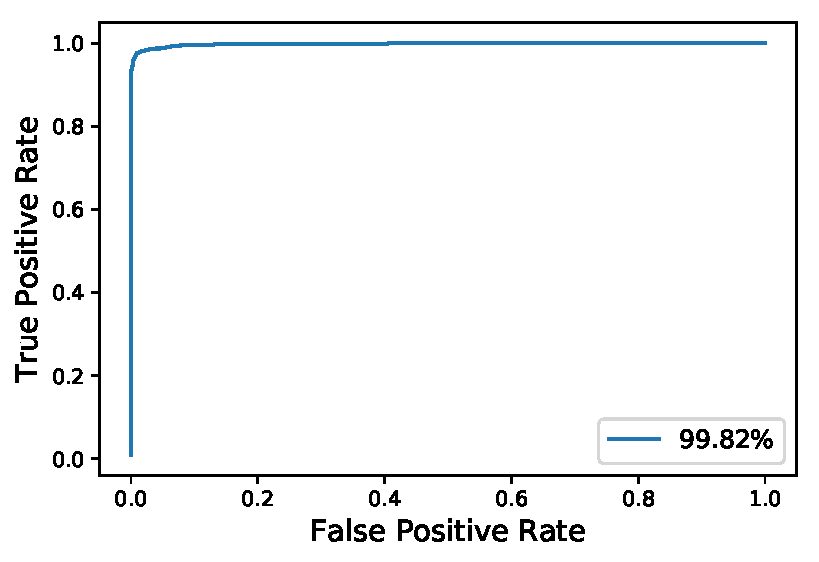
\includegraphics[width=\textwidth]{Figures/Chapter5/SNAGNNoiseROC.pdf}
  \caption{ROC curve and the AUC showing the accuracy, reflecting the high quality of the SN vs AGN vs Noise ML model introduce in this section.}
  \label{fig:AGNNoiseROC}
\end{figure}

\subsubsection{Selecting SNe}
After the numerous preparation steps, we can now obtain classifications for each real, unlabelled DES transient. 19,500 objects were sanitised and reshaped using the same method as the training sample before being passed through the classification network. Amongst this sample, 6000 objects received a classification of `most-likely' being a SN, e.g their probability was highest for this label.

To test the classification model and determine a probability threshold that would ensure a high purity of the sample, I use the samples of spectroscopically classified SNIa, CCSN, SLSNe and AGN as a ground-truth sample. Regardless of their subclass, all confirmed SN in the sample were correctly classified using our CNN and all AGN were also correctly accounted for. Furthermore, each confirmed SN has been identified with a very high degree of confidence exceeding 99\% in the worst cases with an average exceeding 99.99\% for the majority of transients. This result confirms that the high degree of accuracy could not be attributed to overfitting or errors in the analysis but was, in fact, the true representation of the quality and the staggering ability for the CNNs to differentiate these classes of transients. The high level of accuracy suggests that a similar project performed on data with lower quality or more incomplete light curves could still result in a positive result paving way for similar methods to be applied in the future astronomical surveys including LSST.

Using the classification probability values measured for the confirmed objects, I set a conservative threshold of 98\% to select objects which are to enter the next stage of my analysis. This retained 5273 objects which are an approximate match to the numbers of SN discoveries expected in DES \citep{Bernstein2012}.

\subsection{Classifying SNe}
Upon the classification of 5273 transients found in the first four years of operation of DES, the next step of the analysis is to attempt to divide these objects into their respective subclasses using only their light curve data. This task is perhaps one of the greatest challenges facing SN surveys to date, with no project ever accomplishing this with a high degree of confidence without the use of reshifting as a modelling prior.

The classification of SN in the absence of the distance prior requires us to focus purely on the morphology of the light curve including its colour and temporal evolution and apparent luminosity as the only available sources of information. These differences may be very subtle for a number of SN classes, most predominantly SN\,Ia and SN\,Ibc, and we, therefore, do not expect to be able to produce a classification model matching the accuracy of that used to identify SN candidates in DES.

\subsubsection{Data preparation and network selection} \label{sec:SNClassificationNetwork}
The training sample used in the classification of SNe is similar to that used in the previous section, albeit consisting of SN light curve only. In order to provide a fair representation for each subclass of objects, I use an equal sample of SN\,Ia, CCSN and SLSN wherein each case 45,000 objects from the training set. In the case of CCSNe, I use an even contribution from both the sample of SN\,II and SN\,Ibc. The data is also sanitised and reshaped using the tools as used in \sref{sec:AGNNoiseSNSample}

To build the SN classification model, I use the approach developed in \sref{sec:AGNNoiseModel} as the benchmark, and modifying that network to suit this more complex problem. Perhaps the most important change was the introduction of the absolute magnitude as one of the input parameters. In the selection of SNe, performed in \sref{sec:AGNNoiseModel}, this was not necessary as the light curve evolution, normalised to one for each object, provides sufficient information to distinguish between these very distinct classes of objects. In the case of SNe, the difference is very subtle relative to the previous model with the luminosity as a function of the colour likely being one of the strongest indicators for each subclass. The absolute luminosity is measured as the maximum flux in each band across all seasons of data. This provides only four additional data point and is, therefore, introduces late into the network in order to provide them with more weight in determining the final classification \fref{fig:SNClassificationNetwork}.

\begin{figure}
  \centering
  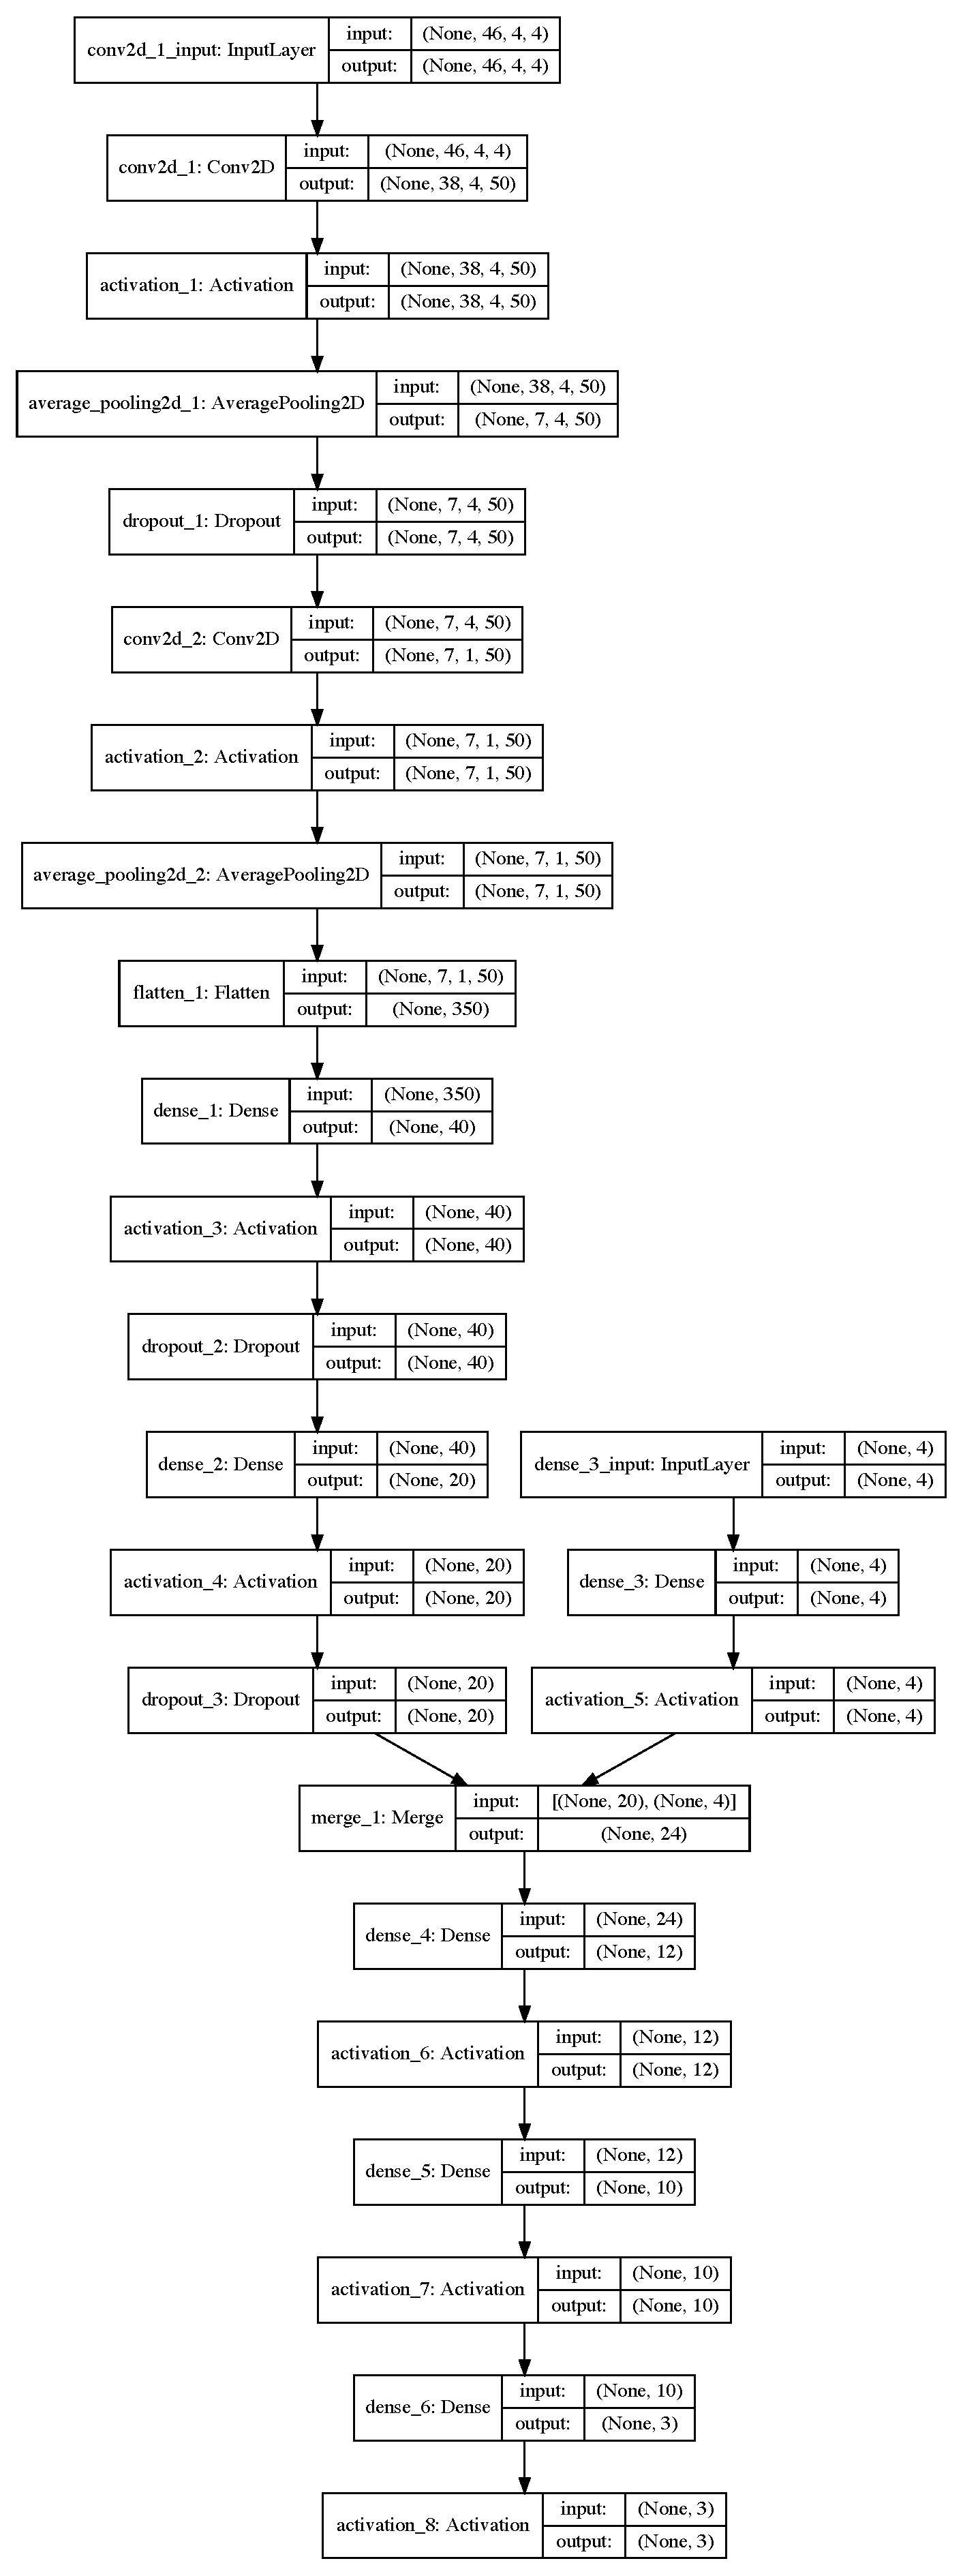
\includegraphics[width=0.6\textwidth]{Figures/Chapter5/SN}
  \caption{The CNN used to subclassify DES SNe amongst their spectral subtypes. This network relies on `Tanh' activation funtions and makes use of the information about the apparent luminosity of the SN, differing from that used in \sref{sec:AGNNoiseModel}}
  \label{fig:SNClassificationNetwork}
\end{figure}

Another important change introduces in this iteration of the CNN was an increase in the number of convolutional filters responsible for measuring the colour of the SN. Through a number of iterations of the model, I found that an increase from 30 to 50 unique filters improves the classification rate by $\sim$3\% without overfitting the model.

Finally, one of the biggest improvements in the model came from modifying the activation function to follow the Tanh distribution over ReLU, introducing an improvement of $\sim$5\%. Interestingly, the same behaviour was not previously observed in the SN identification network where the use of Tanh or Sigmoidal activation functions hinders the classification rate. One possible explanation of this comes from the fact that the differences between the objects in the training samples in the SN identification sample are so large that they require a more flexible and forgiving activation function such as ReLU, while the similarity of the SN subclasses requires a very sensitive, high gradient function to be used. The benefit of the Tanh over a Sigmoid is the scaling between the negative and positive unity as opposed to zero and one, which allows for objects with small negative values.

\subsubsection{Training the model} \label{sec:SNClassification}
Using the training sample and the CNN developed in \sref{sec:SNClassificationModel}, I built a SN classification model that, with an accuracy of 90\%, is one of the most successful SN classifiers to date, despite its independence from any distance priors. At the stage of classifying a purified sample of SNe, our result can be directly compared with \citet{Lochner2016}. Our AUC measured at 97.9\% for SN\,Ia marginally exceeds that of the best result found in \citet{Lochner2016}. However, this does not tell the full story as the best model found in their work sufferers largely from overfitting and the more correct value, found using a larger (albeit non-representative of all subclasses) sample is closer to $\sim$85\%. The accuracy of our classifier is again a testament to the power of CNNs, demonstrating that a similar model could be used in future surveys such as LSST.

\begin{figure}
  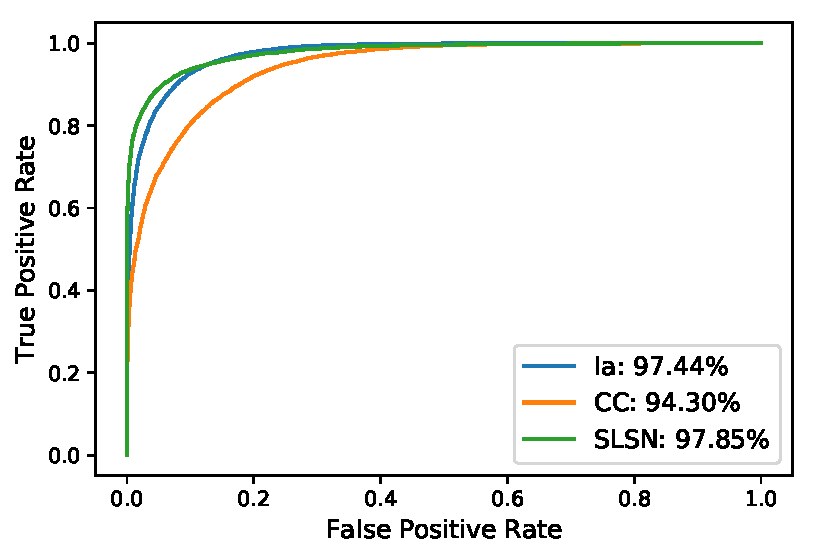
\includegraphics[width=\textwidth]{Figures/Chapter5/SNROC.pdf}
  \caption{The ROC and AUC measured for the SN photometric classification model shown separately for each class of SN present in our training sample.}
  \label{sec:SNClassificationROC}
\end{figure}

\subsection{SLSNe in DES}
Before the SN classification model can be applied to the sample of DES SN candidates, identified in \sref{sec:SNClassification}, it must first be tested against the ground-truth sample of spectroscopically confirmed objects detected by DES. While the model shows that a high degree of precision, it is possible that mistakes in the creation of the artificial training sample could lead to some subclasses not being represented correctly in the classification model.

\subsubsection{Ground-truth sample} \label{sec:SNTruth}
Amongst the sample of 250 spectroscopically confirmed SN\,Ia, 243 are correctly classified in this work. This, in fact, exceeds the value expected from the raw accuracy figures which are likely explained by the spectroscopically confirmed objects being easier to classify than some objects that may lay at the detection limit of the survey.

With this positive result, I apply the same method to SN\,Ib/c and SN\,II. Here the results begin to shed a light on a major issue uncovered in this section. While a majority of the SN\,Ib/c have been correctly identified, a number of SN\,II is have been misidentified as SLSN. The visual inspection of these objects shows that they are exclusively SN\,IIP with, particularly slow descent times. This is a subclass of objects which was not represented at all in the training sample due to the lack of sufficient data. At the current time, using the data available in the literature is not possible to expand our training set with examples of SN\,IIP. However, in \cref{Chapter6} I investigate other approaches, centred around the concept of Unsupervised ML to separate these two groups of transients and provide a pure sample of SLSN.

As the final check, I test the sample of DES SLSNe and find that only 12 of the 18 objects are fully recovered by the model. While at the first glance, this result appears to be in contradiction with the predicted accuracy of the classifier, two of these objects are knows to be only tentatively classified as SLSN (DES15C3hav, DES14C1rhg). Three objects are known not to be a good match to the magnetar model under any assumptions tested in \sref{sec:MagnetarModel} (DES13S2cmm, DES14S2qri). It is harder to postulate why DES16C3ggu and DES15X1noe are not part of the sample. While is possible that their late-season detection is at fault, however, we see that behaviour from a number of objects which are correctly classified.

\begin{table}
  \caption{Percentage probability of the spectroscopically confirmed DES SLSNe as found in the ML photometric classification presented in this chapter.}
  \label{tab:SLSNTruth}
  \centering
  \begin{tabular}{l|r|r|r}
    SN Name & SN\,Ia & CCSN & SLSN \\
    \hline
    DES13S2cmm & 0.04\,\% & 89.18\,\% & 10.77\,\% \\
    DES15X3hm  & 5.65\,\% & 7.40\,\% & 86.95\,\% \\
    DES14X3taz & 1.71\,\% & 2.25\,\% & 96.04\,\% \\
    DES15S2nr  & 0.01\,\% & 0.54\,\% & 99.46\,\% \\
    DES14C1fi  & 0.00\,\% & 0.11\,\% & 99.89\,\% \\
    DES14X2byo & 0.01\,\% & 0.10\,\% & 99.89\,\% \\
    DES15C3hav & 46.10\,\% & 10.38\,\% & 43.52\,\% \\
    DES14C1rhg & 0.87\,\% & 96.90\,\% & 2.23\,\% \\
    DES14S2qri & 2.92\,\% & 90.66\,\% & 6.43\,\% \\
    DES14E2slp & 0.28\,\% & 1.85\,\% & 97.87\,\% \\
    DES15E2mlf & 0.00\,\% & 0.23\,\% & 99.77\,\% \\
    DES15X1noe & 3.63\,\% & 52.81\,\% & 43.56\,\% \\
    DES15S1nog & 19.93\,\% & 14.05\,\% & 66.02\,\% \\
    DES16C3cv  & 0.00\,\% & 0.04\,\% & 99.96\,\% \\
    DES16C2nm  & 0.00\,\% & 0.05\,\% & 99.95\,\% \\
    DES16C2aix & 0.05\,\% & 46.19\,\% & 53.76\,\% \\
    DES16C3dmp & 9.60\,\% & 3.51\,\% & 86.89\,\% \\
    DES16C3ggu & 85.20\,\% & 11.52\,\% & 3.28\,\%
  \end{tabular}
\end{table}

\subsubsection{SN classification}
I applied the final classification model to the 5273 objects real DES objects, previously identified as SN candidates. At the 50\% accuracy threshold, 3192 objects were identified as SN\,Ia which matches the expected values found in \citep{Bernstein2012}, 1389 objects were identified as CCSN which again does not exceed our expectations. The remaining 509 objects were identified as SLSN.

This largely exceeds the numbers expected from the rate of SLSN and is known to be contaminated with long duration SN\,II. However, as the classification model was shown in \sref{sec:SNTruth} to be able to identify a number of known SLSN with a high degree of accuracy (\tref{SLSNTruth}), we have a strong degree of belief that there are in fact numerous SLSN hidden in this contaminated sample that may be recoverable using further analysis, as presented in \cref{Chapter6}

\section{Summary}
In this chapter, I described the approach used in building a training sample of transients resembling the sample of real transients observed by the DES. I used the SNANA generated sample of SN\,Ia. The CoCo and SLAP packages, developed in \cref{Chapter4}, were used to create samples of CCSN and SLSNe respectively. Furthermore, I use a sample of AGNs generated for a similar study in \citet{Hoenig2014} and a basic model of spurious noise detections to generate a DES-like sample of real transients and their contaminants. I use the approach similar to that found in SNANA to apply the survey noise to the modelled light curves before augmenting them to a uniform cadence using GPR, previously discussed in \sref{sec:Augmentation}.

This training sample was used to develop a classification pipeline for photometrically identifying a sample of real SN candidates in DES. This was performed in conjunction with the state of the art CNN algorithm. A similar approach was subsequently used to create a SN photometric classification tool. Our testing suggests that it is one of the most powerful tools of its kind currently available. I applied it to the DES dataset identifying 3192 SN\,Ia, 1389 potential CCSN and a sample of 500 SLSN, although we understand that this sample is heavily contaminated by SN\,IIP which were not included in the original training sample.
 % Experiment 2

%% Chapter 6

\chapter{Results of ML} % Write in your own chapter title
\label{Chapter6}
\lhead{Chapter 6. \emph{High z SLSN}} % Write in your own chapter title to set the page header


\section{First section}
High Z SLSN stuff % Results and Discussion

%\chapter{Conclusions}
\label{Chapter7}
\lhead{Chapter 7. \emph{Conclusions}}

\begin{figure}[H]
  \centering
  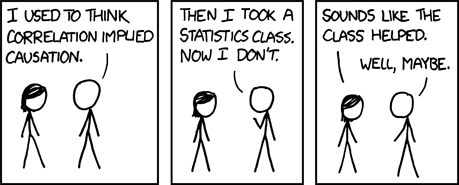
\includegraphics[width=0.6\textwidth]{Figures/xkcd/chapter7.png}
  \caption*{xkcd.com/552}
\end{figure}

In this thesis I have endevoured to demonstrate the possibility of photometrically classifing SLSNe amongst large samples of transients detected by modern, wide-field astronomical surveys. In the process, I have combined our understanding of this class of objects with state-of-the-art Machine Learning and light curve modelling techniques to both define and predict their behaviour in a number of surveys. All this was performed with the aim of broadening our understanding of SLSNe as a population. The main results are summerised below.

\section{Modelling SN light curves}
In \cref{Chapter3}, I described the methods for modelling of a variaty of SN and other transients light curves.

\subsection{Modelling SLSNe}
Since their earliest detections, SLSN SEDs have been known to resemble a black-body continuum, presenting absorption lines only in the UV parts of the spectrum. In this thesis, I demontrate that it is infact possible to produce a high quality SLSN light curve model based on the black-body approximation uppon introducing a spectral absorption template. the evolution of the bolumetric luminosity of SLSNe are based on the birth and spin-down of a magnetar model which I show to correctly represent all literature SLSN examined in this thesis.

\subsection{Modelling CCSN}
In this thesis, I have developed a set of tool for the modelling and of CCSN. As the number of previously available spectroscopic templates used to simulate objects were low, we used the publically available data for both stripped-envelope and hydrogen-rich CCSNe to construct our own sample. While a numer of light curve models were investigated, I found the simple treatment, similar to \citet{Bazin2009}, to be the most robust approach to the problem of modelling and interpoalting of CCSN light curves. Upon flux correcting the available spectroscopy to the observed photomtry, I extended the SED in both IR and UV regimes using a combination of auxillary \textit{Swift}-UVOT data and modelling their continuum as dust extincted black-bodies.

\subsection{Light Curve interpoaltion using Gaussian Processes}
One of the biggest challenges overcome in this thesis was the problem of interpolating transient light curves. Using Gaussian Process Regression, I developed a method which allowes me to probabilistically inperpolate the data without introducing any models which biases the results or correlates them beyond the standard covariance associated with the uncertainties of the photometric points. This was applied to the light curve of every transient detected by DES as well as all atrificially generated objects in the ML training sample created in \cref{Chapter5}

\section{Rates of SLSN}
Motivated by the low number of its measurements, \cref{Chapter4} of this thesis focused on measuring the rate of SLSNe at the intermediate redshift of z$\sim$1, providing one of the most accurate measurements of and allowing us to, for the first time, probe the evolution in the rate of SLSNe.

\subsection{Defining SLSNe}
As the foundation for theis, I used the spin-down of a magnetar model to postulate a definition the SLSNe. After fitting theie literature training sample with the model, I found that the objects concentrate in a small region of the P$_{ms}$-B$_{14}$-$\mathrm{\tau}_M$ parameter space. I defined this region using an ellipsoid which tightly encapsules all object, and can be used to select further objects of this class.

\subsection{Search for SLSN in SNLS}
Using the magnetar model, I fit all SNLS transients and determined that three of these objects fall within the definition fo a SLSN. Two were the previously discovered, spectroscopically confirmed objects: SNLS06D4eu and SNLS07D2bv. However one object, SNLS07D3bs, was previously unclassified. My modelling suggested a good match to a SLSNe at 0.6$<$z$<1$. Upon this descovery we have uncovered an archival spectrum taken during the life of the transients which shows the redshift to be z=0.74, confirming the object to be consistent with a luminosity of a SLSN.

\subsection{Rate of SLSNe at z$\sim$1}
Bassed on the three SLSN objects detected by SNLS, I performed a Monte Carlo simulation of SNLS to determine the rate of SLSNe and its probaility distribution. I reversed the common approach of weighing each objects by its detection efficiency and observed volume and instead simulated SLSNe and they detectibility starting from a rate informing the number of objects placed in my simulated survey and measuring their detected numbers. I find the rate of SLSNe at z$\sim$1 to be $91^{+76}_{-36}$\,SNe\,Yr$^{-1}$\,Gpc$^{-3}$ or 2.2$^{+1.8}_{-0.9}\times10^{-4}$ of the CCSN rate. This is consistent with other, similar pulications and tentitively demonstrates that the rate of SLSNe follows that of the star formation rate of the universe.

\section{Photometic classification of SN}
Photometric classification of SNe forms the center piece of this thesis. Performed using a number of method, I demonstrate that the ML apprach is by far the most powerful approach to the problem, albeit, not the most straightforward to implement as it required the construction of a large, artificial training sample. In this thesis, I present a self-contained solution, starting from historical data used as templates upon which I built the model for CCSN and SLSNe. Based on this I simulate large numbers of light curves and feed them into a CNN classifier, resulting in the classification of all DES transienst.

\subsection{Training sample}
Using the models of readily available models for SN\,Ia and AGNs, custum build models of SLSNe and CCSN, DES noise models and data augmentation using GPR, I have build a large training sample of SN matching the properties of the the real DES transient sample. Consisting $\sim$300,000 object, this is the largest to date light curve sample used for a photometric classification study and represents objects from the edge of detectibility by DES to local objects.

\subsection{Machine Learning Model}
In order to optimise the classification process, the machine learning models have been divided into two classes. First I worked to create a pure sample of SN-like events in combining the samples of various SN subclasses into a single label classified against the smaple of AGN and spurious survey noise. This produces a classification rate of 99.81\%, as measured on the subsample of the training data, as was further validated using the ground-truth sample of spectroscopically confirmed SLSNe which were all correctly identified in this work.

Upon the identification of a sample of DES SN, consiting of 5273 objects, I attemted to subclassify these objects using only SN light curves as the labeled training set. This again produces a strong classification model, capable of correctly identifying nearly all spectroscopically confirmed SN\,Ia. Applying this to the sample of DES transients I found 500 SLSN candidates, a number which vastly exceeds our expectations based on the rate measured in \cref{Chapter4}. Visual instection of the data showed that the sample is heavily contaminated by SN\,IIP which lacked in our training sample due to the low quality of their available spectral series.

\section{Selecting SLSN}
text

\section{Future Work}
text

\subsection{Expanding the Training Sample}
text

\subsection{Rates of SLSNe from DES}
A natural extention of the work undergone in Chapters \ref{Chapter4}-\ref{Chapter6} is to compute the rate of SLSN using this new and expanded sample of objects. The improvement from 3 to XX objects alone will result in a vastly descred uncertainties in the overall rate of SLSNe. However, more importantly it will be the first ever measurement that will allow for a separation of the rate into separate reshift bins using a homogeneus sample.

....

\subsection{Selecting SLSN in LSST}
While 

\subsection{Redshift estimation for photometric SN\,Ia in DES}
Perhaps one of the most interesting results of this thesis, not directly related to its main subject of SLSNe, is the accuracy of photometric selection of SN\,Ia that was obtained purely as a by product of the main analysis. It is worth noting here that the model used for SN\,Ia only included cosmologically
 % Conclusion

%% ----------------------------------------------------------------
% Now begin the Appendices, including them as separate files

\addtocontents{toc}{\vspace{2em}} % Add a gap in the Contents, for aesthetics

\appendix % Cue to tell LaTeX that the following 'chapters' are Appendices

\chapter{Light Curves of SLSNe in DES}
\label{AppendixA}
\lhead{Appendix A. \emph{DES SLSN Light Curves}}

\begin{figure}[H]
  \centering
  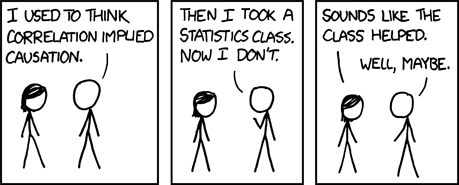
\includegraphics[width=\textwidth]{Figures/xkcd/appendix.png}
  \caption*{xkcd.com/552}
\end{figure}

\section{Light Curves of Photometrically Classified SLSNe in DES}
Below, I include the light curves of SLSNe classified using the ML photometric classification method developed in Chapter \ref{Chapter5}.

\begin{figure}[H]
  \centering
  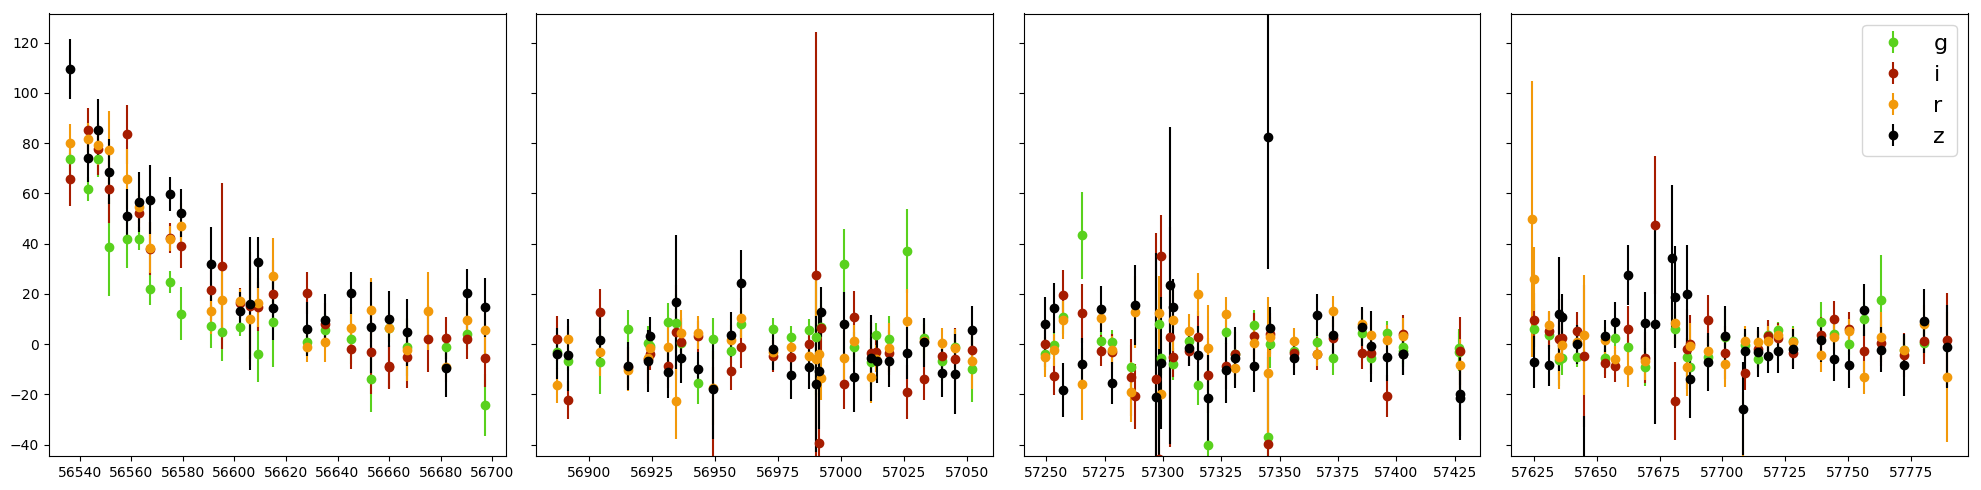
\includegraphics[width=\textwidth]{Figures/Appendix/CNN/1247904.png}
  \caption{DES13X2eti}
\end{figure}

\begin{figure}[H]
  \centering
  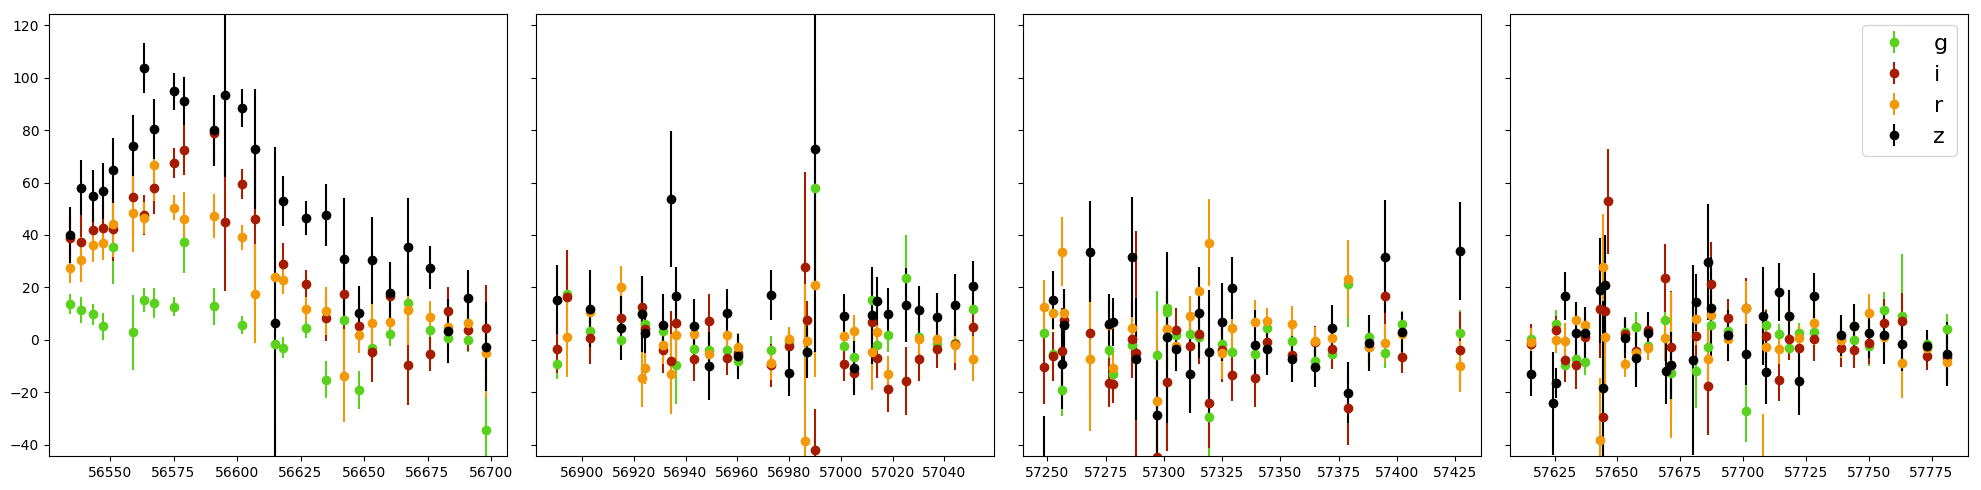
\includegraphics[width=\textwidth]{Figures/Appendix/CNN/1249610.png}
  \caption{DES13X1ayr}
\end{figure}

% \begin{figure}[H]
%   \centering
%   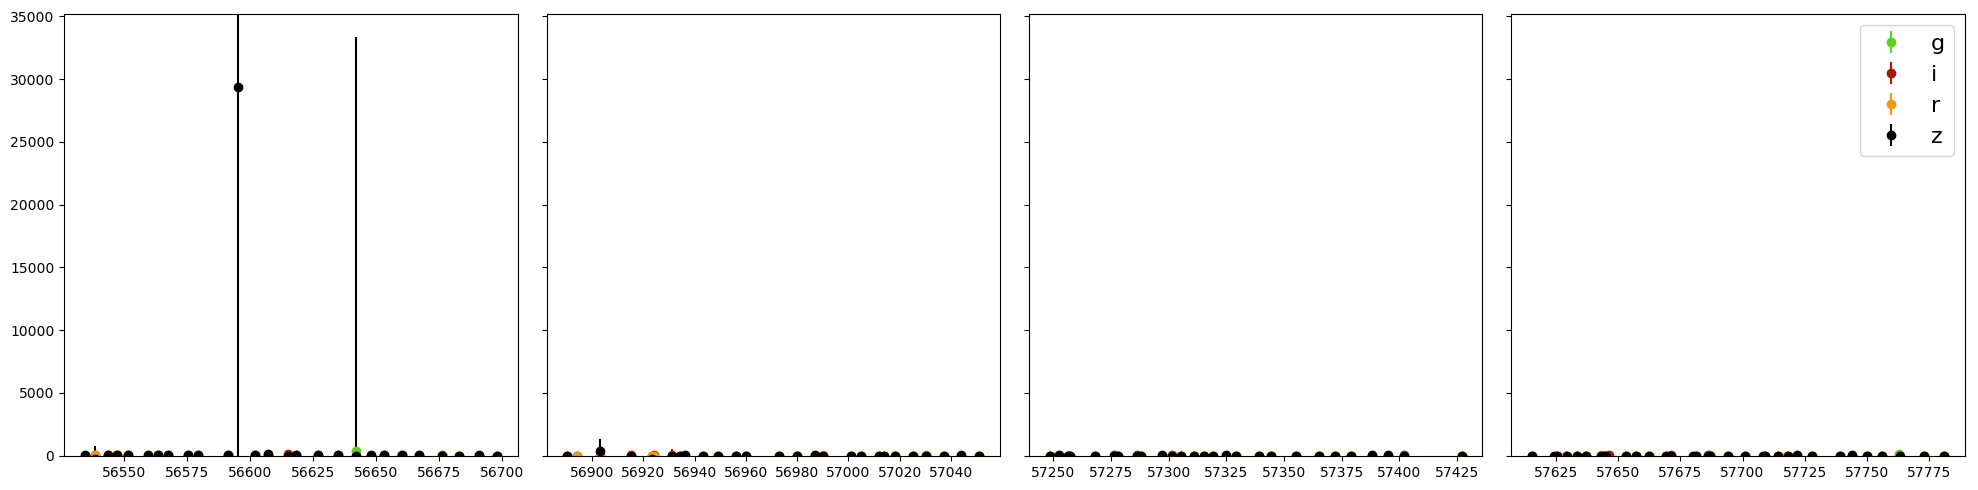
\includegraphics[width=\textwidth]{Figures/Appendix/CNN/1254314.png}
%   \caption{DES13X1csy}
% \end{figure}

\begin{figure}[H]
  \centering
  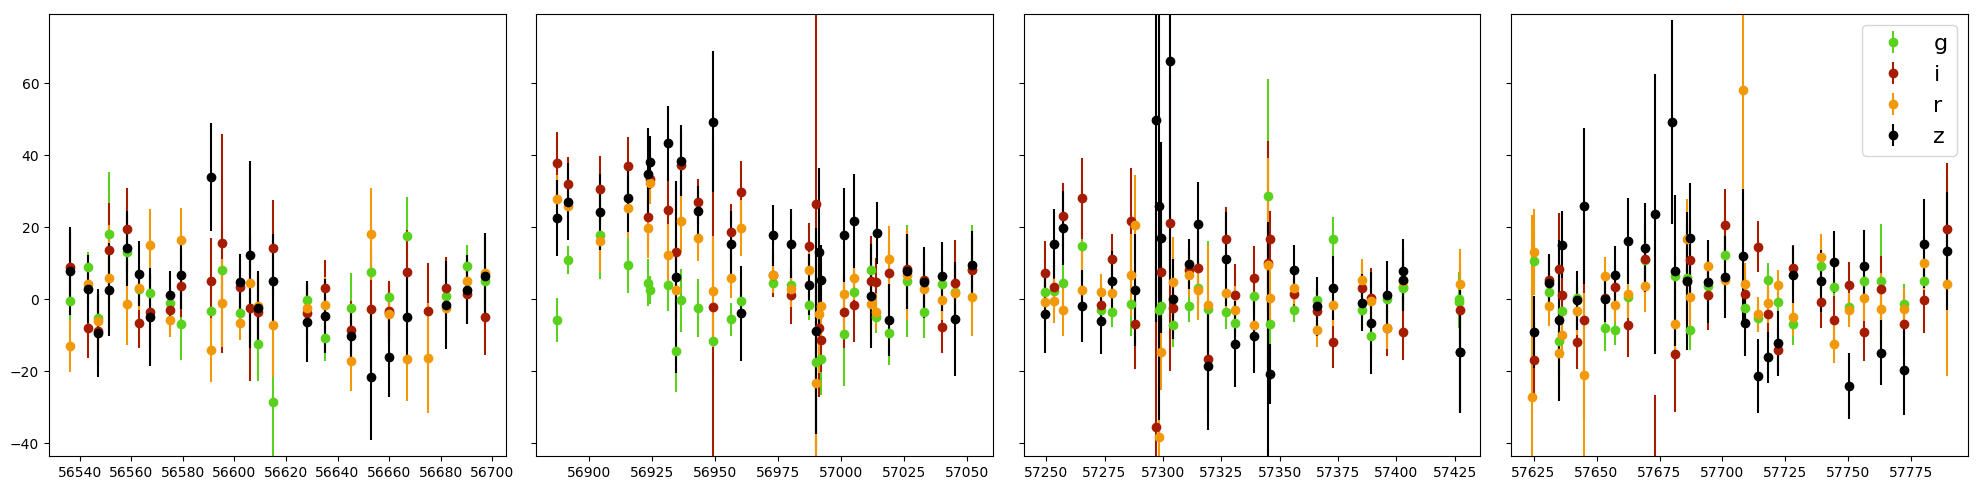
\includegraphics[width=\textwidth]{Figures/Appendix/CNN/1291713.png}
  \caption{DES14X2eb}
\end{figure}

\begin{figure}[H]
  \centering
  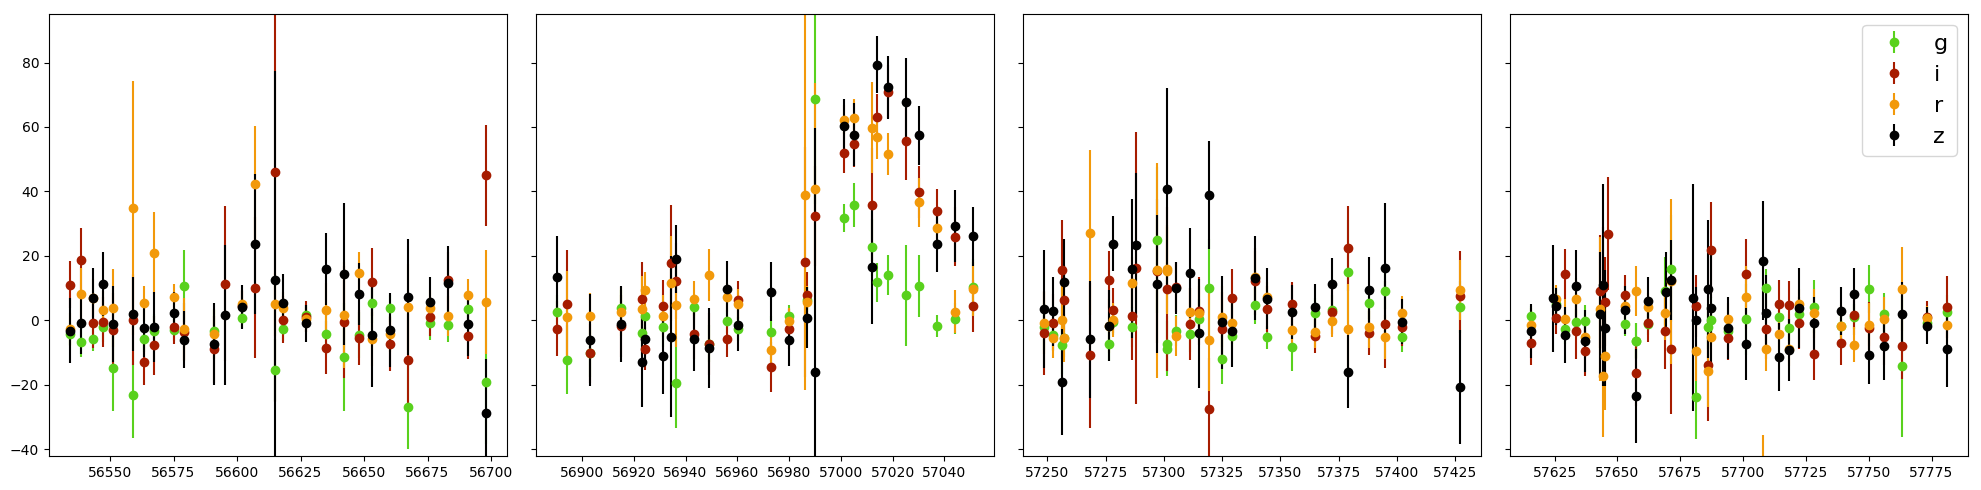
\includegraphics[width=\textwidth]{Figures/Appendix/CNN/1316853.png}
  \caption{DES14X1qzi}
\end{figure}

\begin{figure}[H]
  \centering
  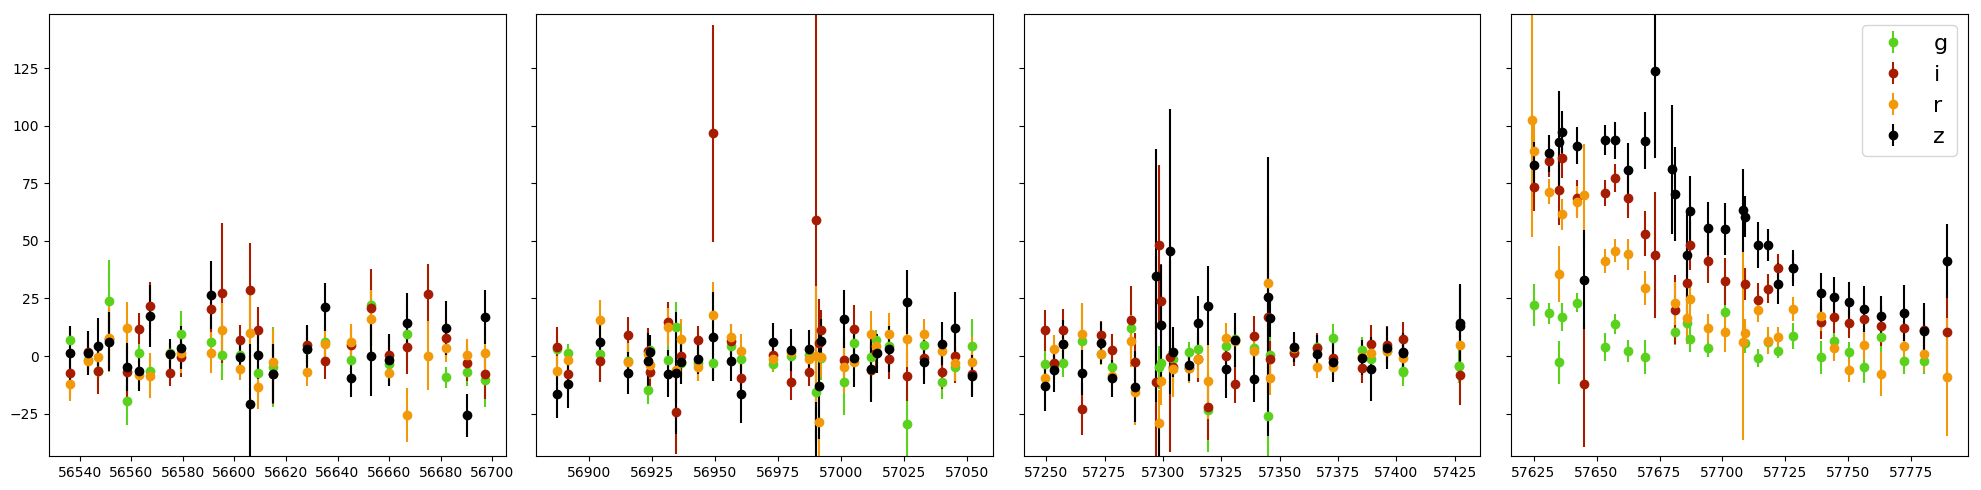
\includegraphics[width=\textwidth]{Figures/Appendix/CNN/1373034.png}
  \caption{DES16X2uq}
\end{figure}

\begin{figure}[H]
  \centering
  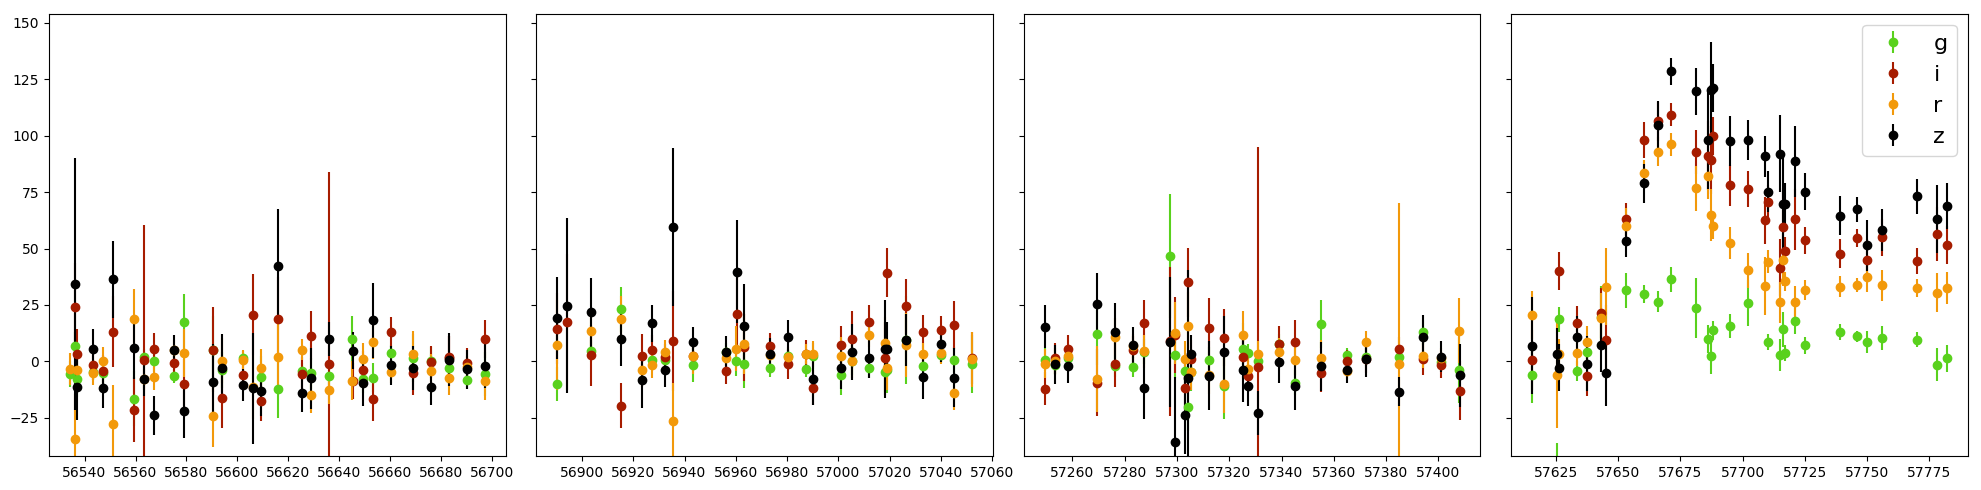
\includegraphics[width=\textwidth]{Figures/Appendix/CNN/1461053.png}
  \caption{DES16S1bzz}
\end{figure}

\begin{figure}[H]
  \centering
  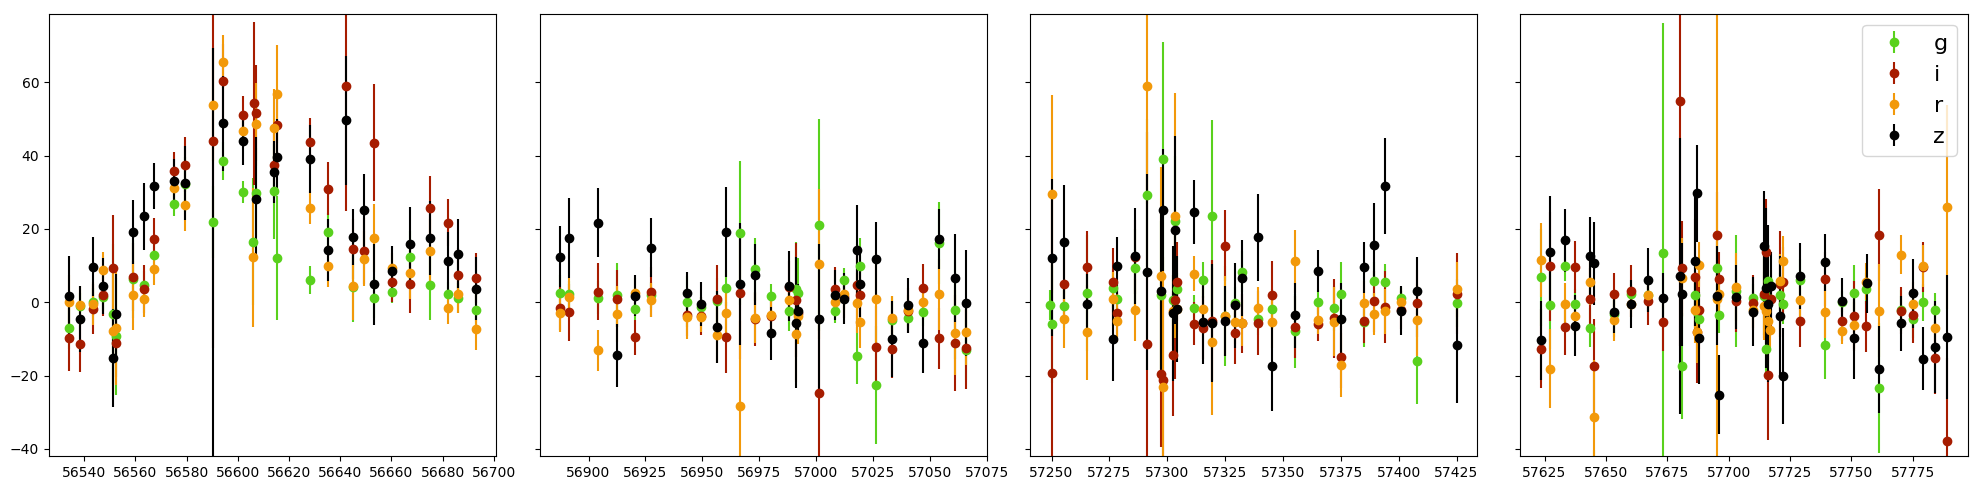
\includegraphics[width=\textwidth]{Figures/Appendix/CNN/1254649.png}
  \caption{DES13C1nln}
\end{figure}

\begin{figure}[H]
  \centering
  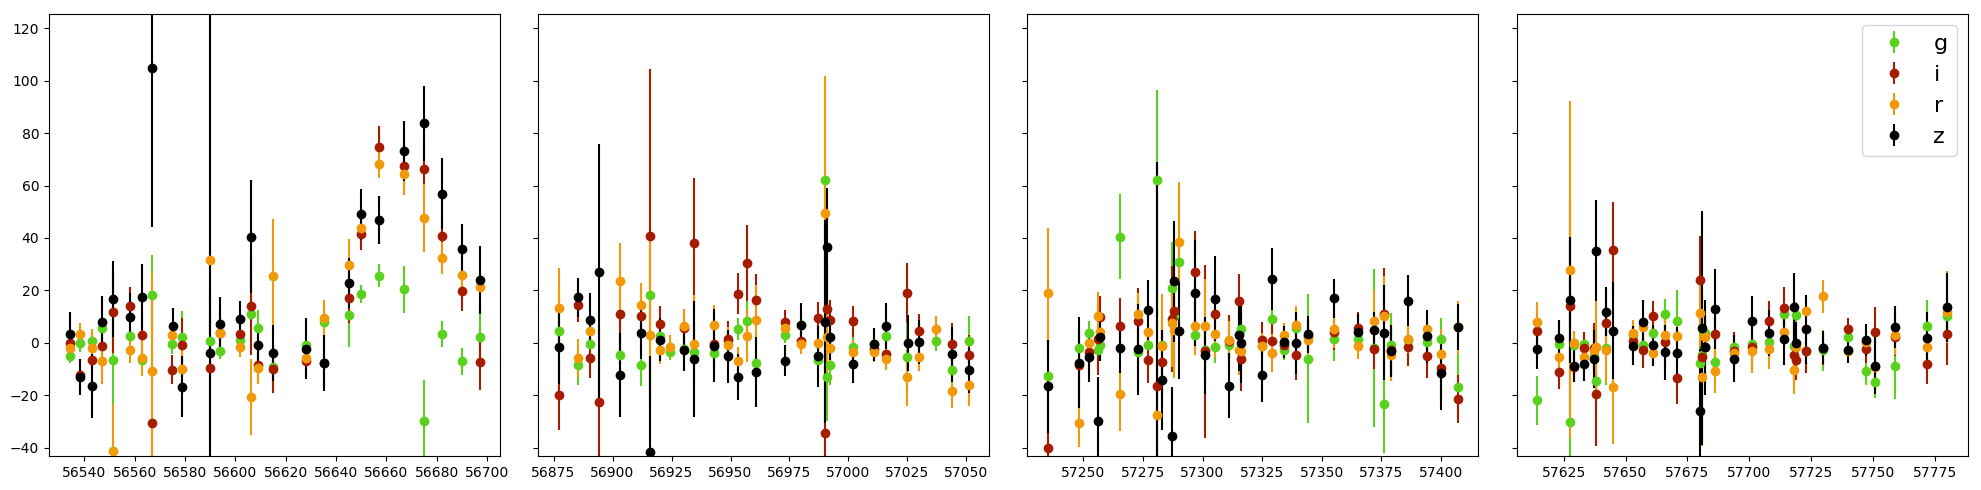
\includegraphics[width=\textwidth]{Figures/Appendix/CNN/1286337.png}
  \caption{DES13E1aftw}
\end{figure}

\begin{figure}[H]
  \centering
  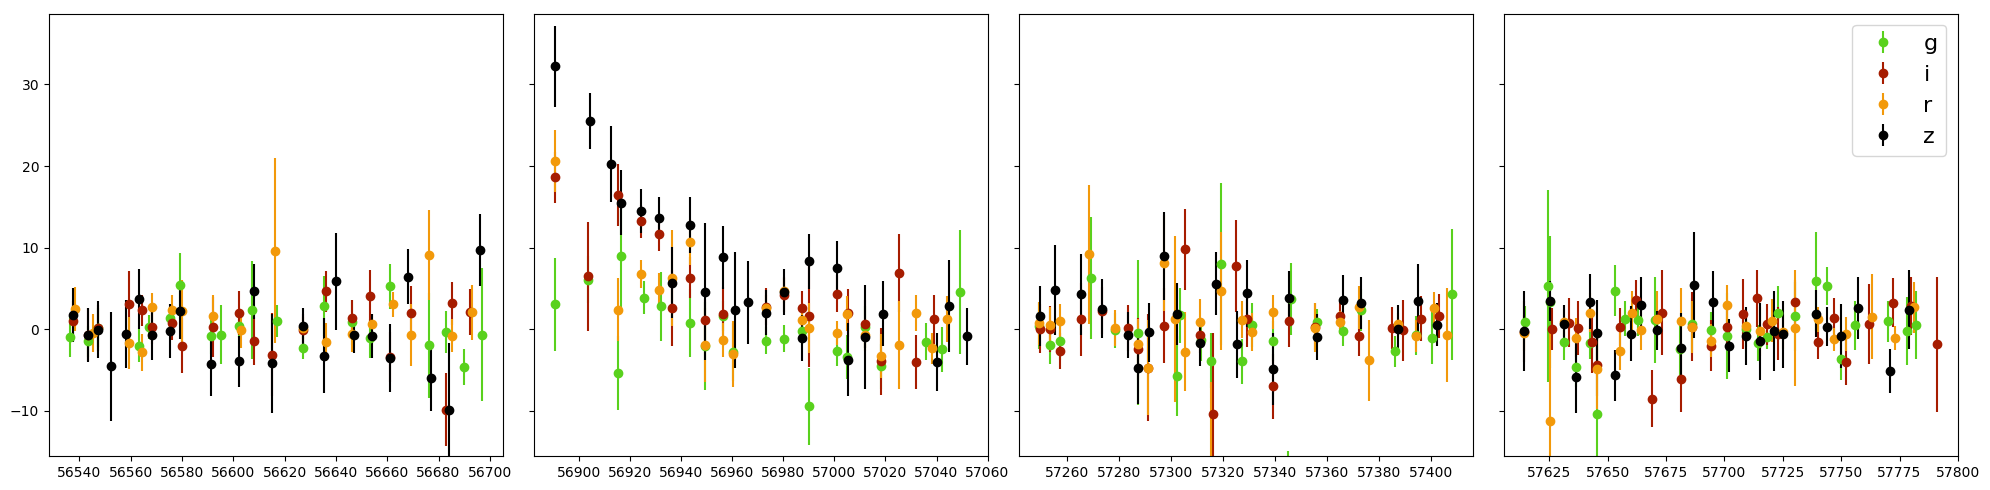
\includegraphics[width=\textwidth]{Figures/Appendix/CNN/1293145.png}
  \caption{DES14X3zq}
\end{figure}

\begin{figure}[H]
  \centering
  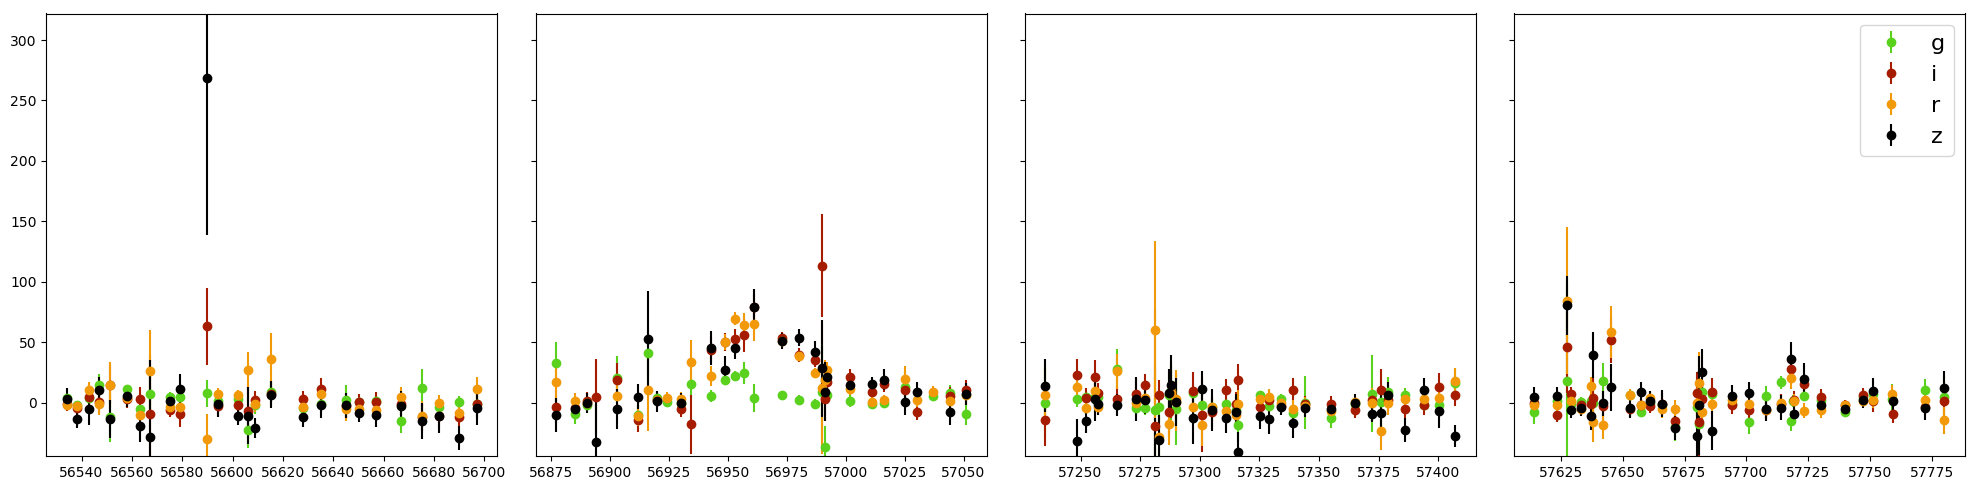
\includegraphics[width=\textwidth]{Figures/Appendix/CNN/1303753.png}
  \caption{DES14E1hek}
\end{figure}

\begin{figure}[H]
  \centering
  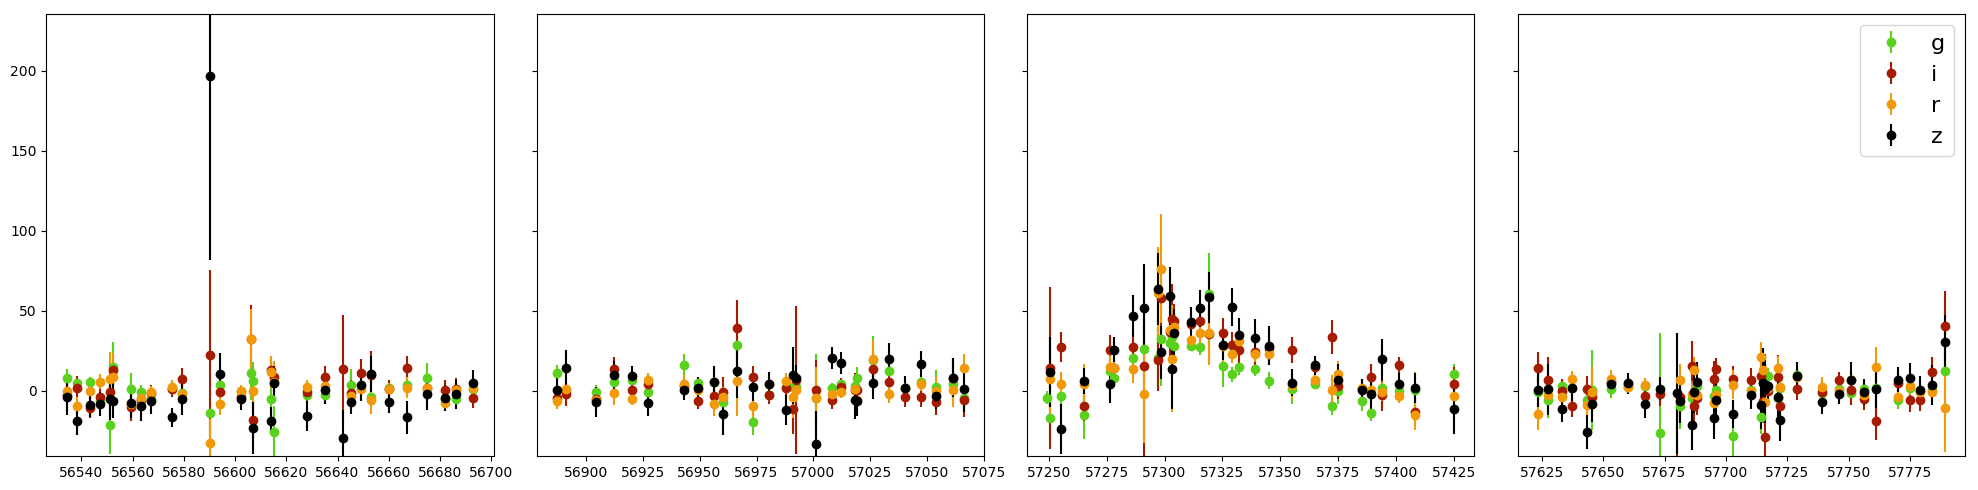
\includegraphics[width=\textwidth]{Figures/Appendix/CNN/1331668.png}
  \caption{DES15C1ljb}
\end{figure}

\begin{figure}[H]
  \centering
  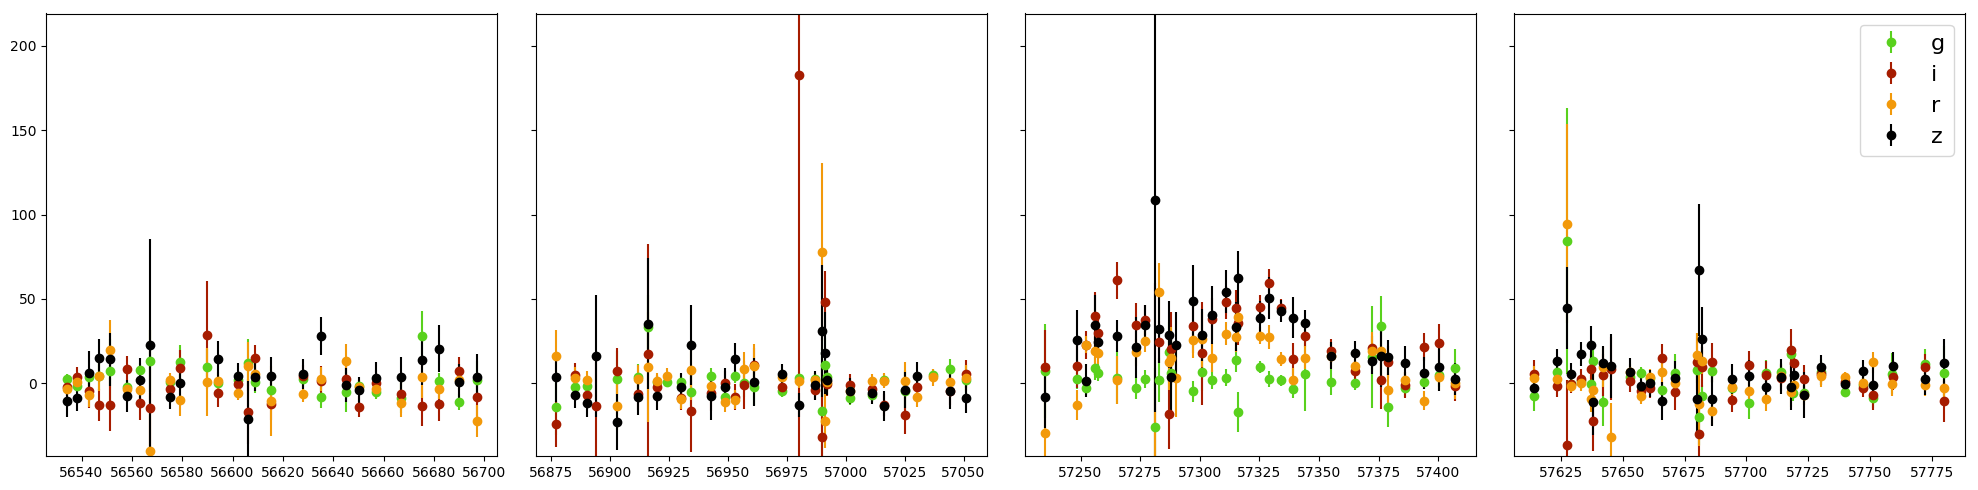
\includegraphics[width=\textwidth]{Figures/Appendix/CNN/1334311.png}
  \caption{DES15E1lwi}
\end{figure}

\begin{figure}[H]
  \centering
  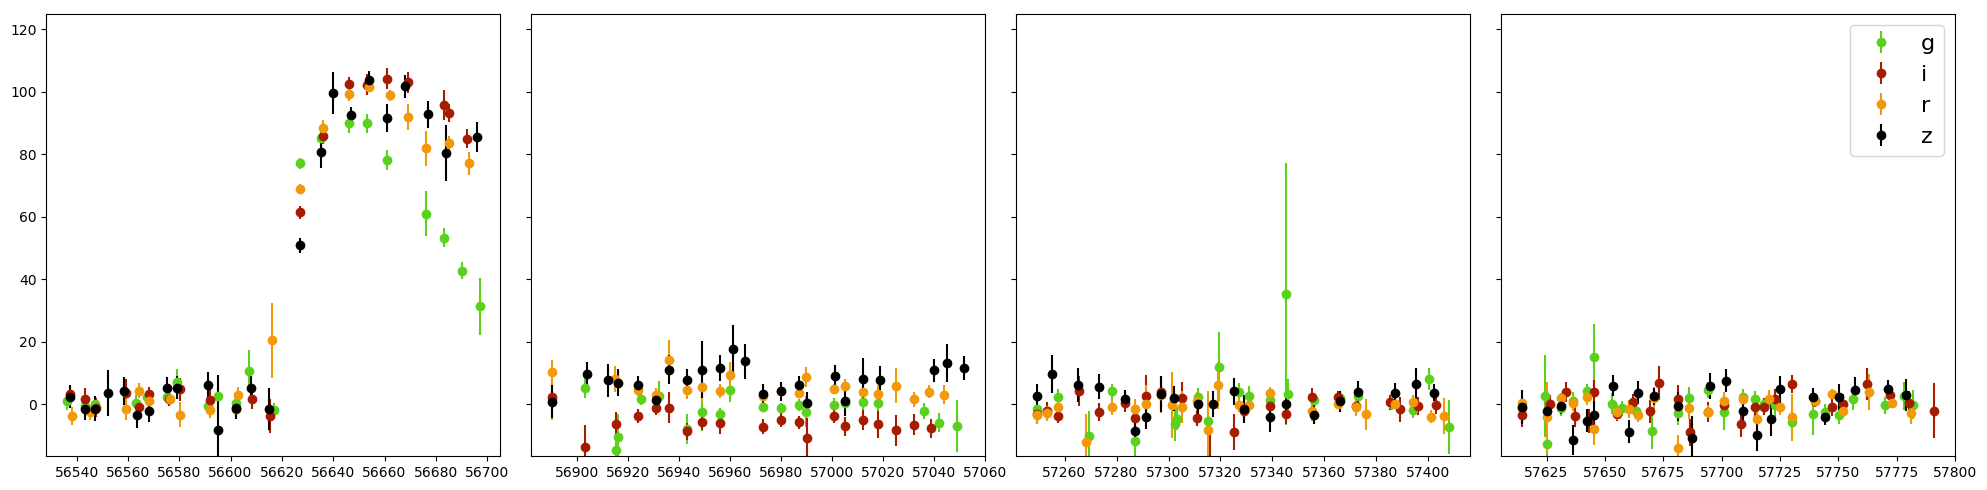
\includegraphics[width=\textwidth]{Figures/Appendix/CNN/1260282.png}
  \caption{DES13X3xyh}
\end{figure}

\begin{figure}[H]
  \centering
  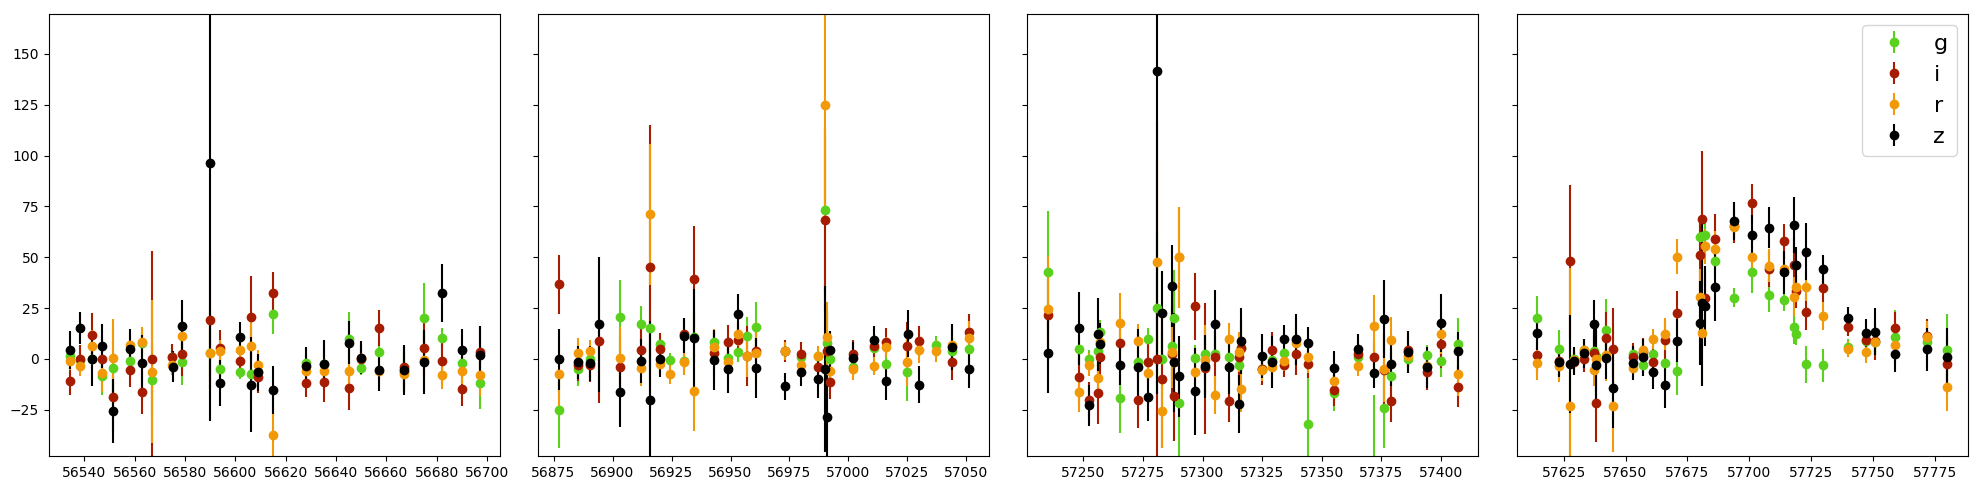
\includegraphics[width=\textwidth]{Figures/Appendix/CNN/1498017.png}
  \caption{DES16E1cjc}
\end{figure}

\begin{figure}[H]
  \centering
  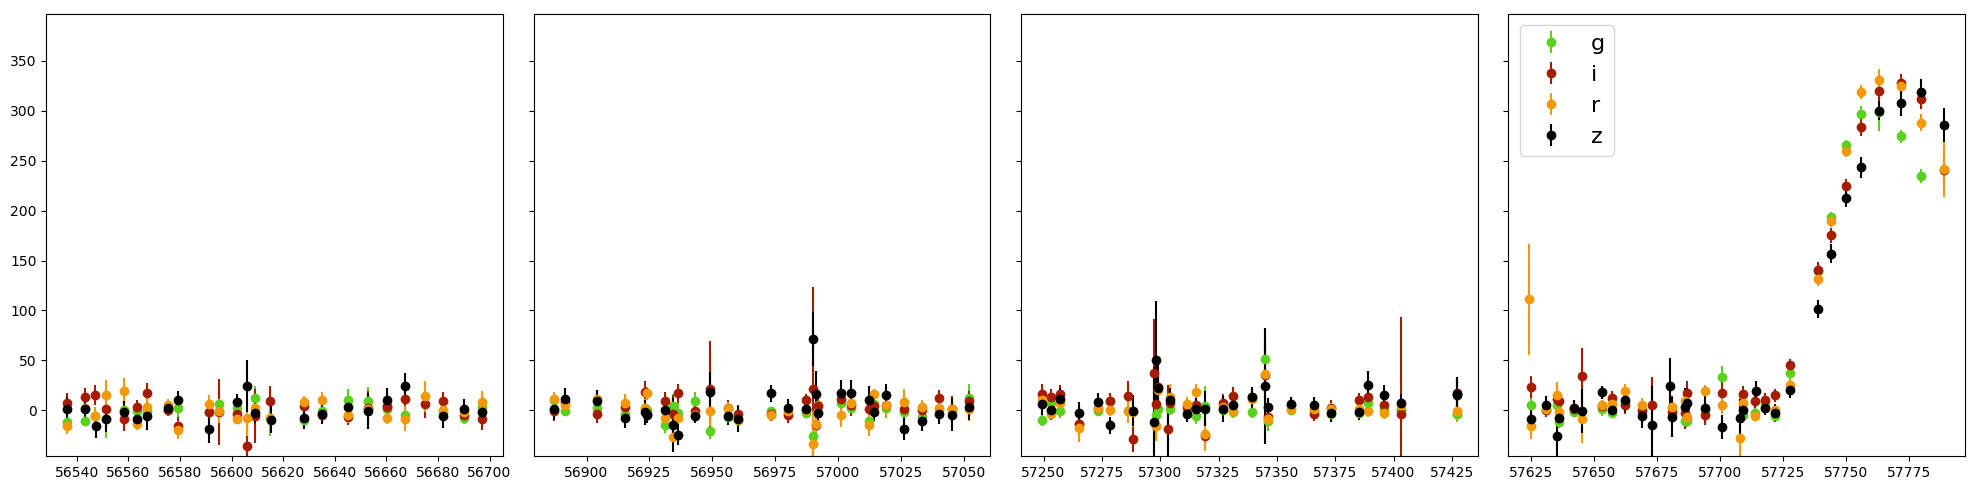
\includegraphics[width=\textwidth]{Figures/Appendix/CNN/1633048.png}
  \caption{DES16X2ewe}
\end{figure}

\begin{figure}[H]
  \centering
  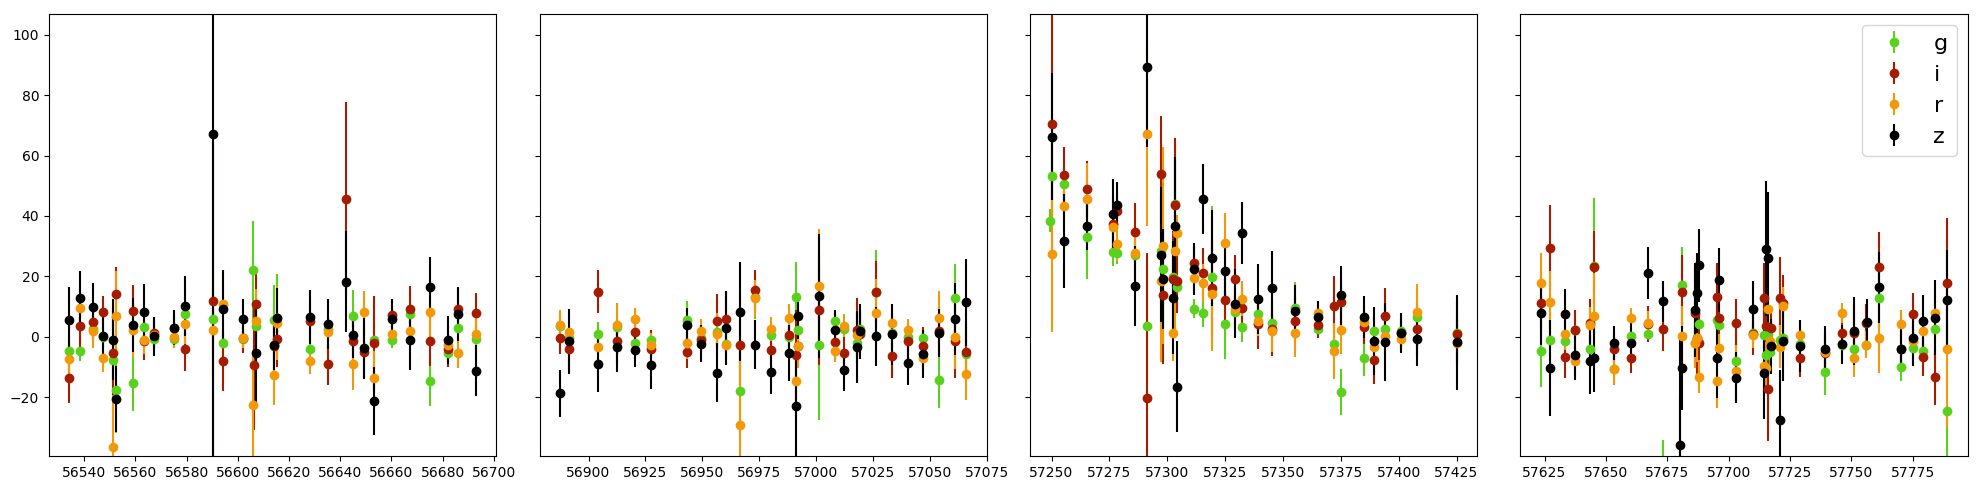
\includegraphics[width=\textwidth]{Figures/Appendix/CNN/1283267.png}
  \caption{DES15C1rq}
\end{figure}

\begin{figure}[H]
  \centering
  \includegraphics[width=\textwidth]{Figures/Appendix/CNN/1262762.png}
  \caption{DES13X3aajk}
\end{figure}

\begin{figure}[H]
  \centering
  \includegraphics[width=\textwidth]{Figures/Appendix/CNN/1655035.png}
  \caption{DES16S2fqy}
\end{figure}

\begin{figure}[H]
  \centering
  \includegraphics[width=\textwidth]{Figures/Appendix/CNN/1255005.png}
  \caption{DES13E1nkg}
\end{figure}

\begin{figure}[H]
  \centering
  \includegraphics[width=\textwidth]{Figures/Appendix/CNN/1258417.png}
  \caption{DES13X3obu}
\end{figure}

\begin{figure}[H]
  \centering
  \includegraphics[width=\textwidth]{Figures/Appendix/CNN/1290501.png}
  \caption{DES14C3aba}
\end{figure}

\begin{figure}[H]
  \centering
  \includegraphics[width=\textwidth]{Figures/Appendix/CNN/1434194.png}
  \caption{DES16X1bhk}
\end{figure}

\begin{figure}[H]
  \centering
  \includegraphics[width=\textwidth]{Figures/Appendix/CNN/1530176.png}
  \caption{DES16X3dlk}
\end{figure}

\begin{figure}[H]
  \centering
  \includegraphics[width=\textwidth]{Figures/Appendix/CNN/1290941.png}
  \caption{DES14C1fs}
\end{figure}

\begin{figure}[H]
  \centering
  \includegraphics[width=\textwidth]{Figures/Appendix/CNN/1306465.png}
  \caption{DES15S1flm}
\end{figure}

\begin{figure}[H]
    \centering
  \includegraphics[width=\textwidth]{Figures/Appendix/CNN/1483027.png}
  \caption{DES16X3cer}
\end{figure}
	% Appendix Title

%\input{./Appendices/AppendixB} % Appendix Title

%\input{./Appendices/AppendixC} % Appendix Title

\addtocontents{toc}{\vspace{2em}}  % Add a gap in the Contents, for aesthetics
\backmatter

%% ----------------------------------------------------------------
\label{Bibliography}
\lhead{\emph{Bibliography}}  % Change the left side page header to "Bibliography"
\bibliographystyle{unsrtnat}  % Use the "unsrtnat" BibTeX style for formatting the Bibliography
\bibliography{Bibliography}  % The references (bibliography) information are stored in the file named "Bibliography.bib"

\end{document}  % The End
%% ----------------------------------------------------------------